\documentclass[twoside, a4paper, 12pt]{book}



%:-------------------------- packages for fancy things -----------------------

\usepackage{amssymb, amsmath}
\usepackage{graphics} % for improved inclusion of graphics
%\usepackage{wrapfig} % to include figure with text wrapping around it
\usepackage[margin=10pt,font=small,labelfont=bf]{caption} % for improved layout of figure captions with extra margin, smaller font than text
\usepackage{fancyhdr} % for better header layout
\usepackage{eucal}
\usepackage[english]{babel}
\usepackage[usenames, dvipsnames]{color}
\usepackage[perpage]{footmisc}
%\usepackage[round, sort, numbers, authoryear]{natbib}
\usepackage{ifthen}
\usepackage{multicol} % for pages with multiple text columns, e.g. References
\setlength{\columnsep}{20pt} % space between columns; default 10pt quite narrow
\usepackage[nottoc]{tocbibind} % correct page numbers for bib in TOC, nottoc suppresses an entry for TOC itself
%\usepackage{nextpage}

\usepackage{lmodern}

\usepackage{listings}

%\usepackage[final]{pdfpages} % for including other pdf-files

%\usepackage[toc, page]{appendix}

\usepackage{algorithmic}
\usepackage{algorithm}
%\usepackage{program}

\numberwithin{algorithm}{chapter}

\usepackage[utf8x]{inputenc}

%:-------------------------- Glossary/Abbrev./Symbols -----------------------

\usepackage[intoc]{nomencl} % load nomencl extension; include in TOC
%\nomrefpage % to include page numbers after abbrevations
\renewcommand{\nomname}{Glossary} % rename nomenclature
\renewcommand{\nomlabel}[1]{\textbf{#1}} % make abbreviations bold
\makenomenclature % used to be \makeglossary
\newcommand{\g}{\footnote{For all abbreviations see the glossary on page \pageref{nom}.}} % type "\g" to refer to glossary




% used to be for sorting into categories:
%\renewcommand\nomgroup[1]{%
%  \ifthenelse{\equal{#1}{A}}{%
%   \item[\textbf{Roman Symbols}] }{%             A - Roman
%    \ifthenelse{\equal{#1}{G}}{%
%     \item[\textbf{Greek Symbols}]}{%             G - Greek
%      \ifthenelse{\equal{#1}{R}}{%
%        \item[\textbf{Superscripts}]}{%              R - Superscripts
%          \ifthenelse{\equal{#1}{S}}{%
%           \item[\textbf{Subscripts}]}{{%             S - Subscripts
%	    \ifthenelse{\equal{#1}{X}}{%
%	     \item[\textbf{Other Symbols}]}{{%    X - Other Symbols
%	    \ifthenelse{\equal{#1}{Z}}{%
%	     \item[\textbf{Acronyms}]}%              Z - Acronyms
%              			{{}}}}}}}}}}



%-------Hyperref and graphics ---------------%
\usepackage[ pdftex, plainpages = false, pdfpagelabels, 
                 pdfpagelayout = useoutlines,
                 bookmarks,
                 bookmarksopen = true,
                 bookmarksnumbered = true,
                 breaklinks = true,
                 linktocpage,
                 pagebackref,
                 colorlinks = false,  % was true
                 linkcolor = blue,
                 urlcolor  = blue,
                 citecolor = red,
                 anchorcolor = green,
                 hyperindex = true,
                 hyperfigures
                 ]{hyperref} 

\DeclareGraphicsExtensions{.png, .jpg, .jpeg, .pdf, .gif} %GIF doesn't work??
\usepackage[pdftex]{graphicx}
\pdfcompresslevel=9
%\graphicspath{{0_frontmatter/figures/PNG/}{0_frontmatter/figures/PDF/}{0_frontmatter/figures/}}


%:-------------------------- page layout -----------------------

%A4 settings

\pdfpageheight=297mm
\pdfpagewidth=210mm


\setlength{\hoffset}{0.00cm}
\setlength{\voffset}{0.00cm}

%: Uncomment this secion for two-sided printing
% ------------------------------
\setlength{\oddsidemargin}{1.5cm}
\setlength{\evensidemargin}{0cm}
\setlength{\topmargin}{1mm}
\setlength{\headheight}{1.36cm}
\setlength{\headsep}{1.00cm}
\setlength{\textheight}{20.84cm}
\setlength{\textwidth}{14.5cm}
\setlength{\marginparsep}{1mm}
\setlength{\marginparwidth}{3cm}
\setlength{\footskip}{2.36cm}


%: Uncomment this secion for one-sided printing
% taken from the original file, but with the first two lanes modified
% ------------------------------
%\setlength{\evensidemargin}{1.9cm} % was 1.96cm in original
%\setlength{\oddsidemargin}{-0.001cm} % was -0.54cm in original file
%\setlength{\topmargin}{1mm}
%\setlength{\headheight}{1.36cm}
%\setlength{\headsep}{1.00cm}
%\setlength{\textheight}{20.84cm}
%\setlength{\textwidth}{14.5cm}
%\setlength{\marginparsep}{1mm}
%\setlength{\marginparwidth}{3cm}
%\setlength{\footskip}{2.36cm}


%: section below defines fancy page layout options
% ------------------------------
\pagestyle{fancy}
\renewcommand{\chaptermark}[1]{\markboth{\MakeUppercase{\thechapter. #1 }}{}}
\renewcommand{\sectionmark}[1]{\markright{\thesection\ #1}}
\fancyhf{}
\fancyhead[RO]{\bfseries\rightmark}
\fancyhead[LE]{\bfseries\leftmark}
\fancyfoot[C]{\thepage}
\renewcommand{\headrulewidth}{0.5pt}
\renewcommand{\footrulewidth}{0pt}
\addtolength{\headheight}{0.5pt}
\fancypagestyle{plain}{
  \fancyhead{}
  \renewcommand{\headrulewidth}{0pt}
}





%:-------------------------- title page layout -----------------------

% starts roman page numbering until chapter 1
% important to avoid two pages numbered 1 and 2 which may cause bad links
% bug: cover i + back side ii and then numbering restarts with i; should be iii
\renewcommand{\thepage}{\roman{page}}

\newcommand{\submittedtext}{{A thesis submitted for the degree of}}

% DECLARATIONS
% These macros are used to declare arguments needed for the
% construction of the title page and other preamble.

% The year and term the degree will be officially conferred
\def\degreedate#1{\gdef\@degreedate{#1}}
% The full (unabbreviated) name of the degree
\def\degree#1{\gdef\@degree{#1}}
% The name of your college or department(eg. Trinity, Pembroke, Maths, Physics)
\def\collegeordept#1{\gdef\@collegeordept{#1}}
% The name of your University
\def\university#1{\gdef\@university{#1}}
% Defining the crest
\def\crest#1{\gdef\@crest{#1}}
% Stating the city of birth for title page where needed; uncommented for use
%\def\cityofbirth#1{\gdef\@cityofbirth{#1}}

% These macros define an environment for front matter that is always 
% single column even in a double-column document.
\newenvironment{alwayssingle}{%
       \@restonecolfalse\if@twocolumn\@restonecoltrue\onecolumn
       \else\newpage\fi}
       {\if@restonecol\twocolumn\else\newpage\fi}

%:-------------------------- front matter layout -----------------------

% DEDICATION
%
% The dedication environment makes sure the dedication gets its
% own page and is set out in verse format.

\newenvironment{dedication}
{
  \pagestyle{empty}
  \begin{center}
  \vspace*{1.5cm}
  {\LARGE }
  \end{center}
  \vspace{0.5cm}
  \begin{quote} \begin{center}}
{\end{center} \end{quote}}


% ACKNOWLEDGEMENTS
%
% The acknowledgements environment puts a large, bold, centered 
% "Acknowledgements" label at the top of the page. The acknowledgements
% themselves appear in a quote environment, i.e. tabbed in at both sides, and
% on its own page.

\newenvironment{acknowledgements}
{\pagestyle{empty}
\begin{center}
\vspace*{1.5cm}
{\Large \bfseries Acknowledgements}
\end{center}
\vspace{0.5cm}
\begin{quote}}
{\end{quote}}

% The acknowledgementslong environment puts a large, bold, centered 
% "Acknowledgements" label at the top of the page. The acknowledgement itself 
% does not appears in a quote environment so you can get more in.

\newenvironment{acknowledgementslong}
{\pagestyle{empty}
\begin{center}
\vspace*{1.5cm}
{\Large \bfseries Acknowledgements}
\end{center}
\vspace{0.5cm}\begin{quote}}
{\end{quote}}

%ABSTRACT
%
%The abstract environment puts a large, bold, centered "Abstract" label at
%the top of the page. The abstract itself appears in a quote environment,
%i.e. tabbed in at both sides, and on its own page.

\newenvironment{abstracts} { \pagestyle{empty}
  \begin{center}
  \vspace*{1.5cm}
  {\Large \bfseries  Abstract}
  \end{center}
  \vspace{0.5cm}
   \begin{quote}}
{\end{quote}}

%The abstractlong environment puts a large, bold, centered "Abstract" label at
%the top of the page. The abstract itself does not appears in a quote
%environment so you can get more in.

\newenvironment{abstractslong} { \pagestyle{empty}
  \begin{center}
  \vspace*{1.5cm}
  {\Large \bfseries  Abstract}
  \end{center}
  \vspace{0.5cm} \begin{quote}}
      {\end{quote}}

%The abstractseparate environment is for running of a page with the abstract
%on including title and author etc as required to be handed in separately

\newenvironment{abstractseparate} {\pagestyle{empty}
  \vspace*{-1in}
 \begin{center}
    { \Large {\bfseries {\@title}} \par}
    {{\large \vspace*{1ex} \@author} \par}
{\large \vspace*{1ex}
    {{\@collegeordept} \par}
    {{\@university} \par}
\vspace*{1ex}
    {{\it \submittedtext} \par}
    {\it {\@degree} \par}
\vspace*{2ex}
    {\@degreedate}}
  \end{center}}
{}

%Statement of originality if required

\newenvironment{declaration} { \pagestyle{empty}
  \begin{center}
  \vspace*{1.5cm}
  {\Large \bfseries  Declaration}
  \end{center}
  \vspace{0.5cm}
   \begin{quote}}
{\end{quote}}


%:-------------------------- page numbers: roman+arabic -----------------------

% ROMANPAGES
%
% The romanpages environment set the page numbering to lowercase roman one
% for the contents and figures lists. It also resets
% page-numbering for the remainder of the dissertation (arabic, starting at 1).

%\newenvironment{romanpages}
%{
%	\setcounter{page}{1}
%	\renewcommand{\thepage}{\roman{page}}
%} % close romanpage env't
 
{\newpage\renewcommand{\thepage}{\arabic{page}}\setcounter{page}{1}}


%: ----------------------------------------------------------------------
%:                  TITLE PAGE: name, degree,..
% ----------------------------------------------------------------------
% below is to generate the title page with crest and author name

%if output to PDF then put the following in PDF header
%\pdfinfo { /Title  (Master Thesis)
%               /Creator (Tex)
%               /Producer (pdfTeX)
%               /Author (Anders Garmo)
%               /CreationDate (Monday:20100617000000)  %format D:YYYYMMDDhhmmss
%               /ModDate (D:YYYYMMDDhhmm)
%               /Subject (xyz)
%               /Keywords (add, your, keywords, here) }
%\pdfcatalog { /PageMode (/UseOutlines)
%                  /OpenAction (fitbh)  }


\title{A Navigation System for a Snakelike Pipe Inspection Robot}



\author{Anders Moen Garmo}

\collegeordept{Institute of Cybernetics}
\university{Norwegian University of Sience and Technology}

% The crest is a graphics file of the logo of your research institution.
% Place it in ./0_frontmatter/figures and specify the width

%\crest{
\includegraphics[width=4cm]{logo.png}}
  
\degree{MSc}
\degreedate{2010 06}


% ----------------------------------------------------------------------
       
% turn of those nasty overfull and underfull hboxes
%\hbadness=10000
%\hfuzz=50pt


%: --------------------------------------------------------------
%:                  FRONT MATTER: dedications, abstract,..
% --------------------------------------------------------------

\begin{document}

%: ----------------------- generate cover page ------------------------

\maketitle  % command to print the title page with above variables


%: ----------------------- tie in front matter ------------------------

\begin{abstracts}
    The abstract needs to be very good. This is what defines what is done and how it went.
\end{abstracts}

\frontmatter

\begin{acknowledgements}
    This is where I thank people. The teachers and professors at my university and my
    girlfriend and family for supporting me.
\end{acknowledgements}



%: ----------------------- contents ------------------------

\setcounter{secnumdepth}{3} % organisational level that receives a numbers
\setcounter{tocdepth}{3}    % print table of contents for level 3
\tableofcontents            % print the table of contents
% levels are: 0 - chapter, 1 - section, 2 - subsection, 3 - subsection


%: ----------------------- list of figures/tables ------------------------

\listoffigures	% print list of figures

\listoftables

%: ----------------------- glossary ------------------------

% Tie in external source file for definitions: /0_frontmatter/glossary.tex
% Glossary entries can also be defined in the main text. See glossary.tex

% this file is called up by thesis.tex
% content in this file will be fed into the main document

% Glossary entries are defined with the command \nomenclature{1}{2}
% 1 = Entry name, e.g. abbreviation; 2 = Explanation
% You can place all explanations in this separate file or declare them in the middle of the text. Either way they will be collected in the glossary.

% required to print nomenclature name to page header
\markboth{\MakeUppercase{\nomname}}{\MakeUppercase{\nomname}}


% ----------------------- contents from here ------------------------

\nomenclature{DOF}{Degree of Freedom}
\nomenclature{AUV}{Autonomous Underwater Vehicle}





\begin{multicols}{2} % \begin{multicols}{#columns}[header text][space]
\begin{footnotesize} % scriptsize(7) < footnotesize(8) < small (9) < normal (10)

\printnomenclature[1.5cm] % [] = distance between entry and description
\label{nom} % target name for links to glossary

\end{footnotesize}
\end{multicols}



%: --------------------------------------------------------------
%:                  MAIN DOCUMENT SECTION
% --------------------------------------------------------------

% the main text starts here with the introduction, 1st chapter,...
\mainmatter

%\renewcommand{\chaptername}{} % uncomment to print only "1" not "Chapter 1"


%: ----------------------- subdocuments ------------------------

% Parts of the thesis are included below. Rename the files as required.
% But take care that the paths match. You can also change the order of appearance by moving the include commands.


\chapter{Introduction}
Making an autonomous robot has been the goal of scientists and engineers for years. This
is a difficult task which includes many disciplines, and has up to date, not been solved in
a general way. Robots which can reason and take own decisions based on how it senses the
environment would greatly simplify our lives in many ways. Many tasks could be completely
outsourced to autonomous robots which do not tier, and is expendable. This means that it
can go places that a human could not. In short this can be summarized into the three Ds,
namely \emph{dull, dirty} and \emph{dangerous} work. Imagine an autonomous robot going
into an earthquake area, mapping out dangerous spots, and where injured people are,
before medical personnel enter the area. Or a robot mapping and inspecting the vast sewer
network of a large city, searching for weak spots and clogged pipes which obstruct the
sewer flow. Or robots crawling the pipelines carrying water, oil or gas to detect leaks
which will cause catastrophic events if not tended to. All of these examples are important work which
is dangerous, dirty or dull, or all three at once.

The problem when a robot is going into an unknown area and mapping the surroundings using
a pack of sensors is formalized into something called \emph{SLAM}, short for
\emph{Simultaneous Localization and Mapping}.
This is a problem that has been thoroughly researched, and has been tried with numerous sensor types
and many solutions are proposed. Some are best in structured environments, like office
landscapes and industrial areas, while other will preform better in more sparse areas with
less landmarks and recognizable features. 

In our global world, the transport of resources, like oil, gas and water are of great importance. Much of this
transport is done using pipelines. There are literally millions of kilometres with pipelines around
the world. Some of these can be inspected from the outside, but most of them are on the
sea floor or under ground and does not allow for outside inspections. 
The pipelines need regular inspections to ensure that the pipeline is intact
and undamaged. Also sewers, as mentioned above, need inspections to keep a satisfactory
standard. Some of the pipes are considered accessible by humans, i.e. diameter over 80 cm,
but most are smaller than this, and uses various inspection devices feeding video to a human
operator that must detect, record, and classify the damages. This is tedious work which
can be automated using robots. \cite{MAKRO-project}

One such robot suitable for pipe inspection might be the \emph{Pipe Inspection Konda}
(PIKo) developed by SINTEF. This is a snake like robot, consisting of a series of identical
modules interconnected by two degrees of freedom active joints. On each module there is a
set of four wheels, two near the ground and two on the top of the modules. For
horizontal motion it uses these wheels and a train like motion to propel itself forward. Since the joints 
connecting the modules have two degrees of freedom, the robot is capable of traversing vertical pipes
as well. This is achieved by spanning the robot inside the pipe alternately and pushing the wheels towards
the pipe walls to gain enough friction for the robot to motion vertically. \cite{piko}

This report will outline a possible navigation system for PIKo. This include the eyes and
ears, the reasoning needed to interpret the senses, together with recollection of the
areas and the decision making on what to do next. Making the robot do this all by it self
is a tremendous task and has up to date not been solved for the general environment.
\begin{figure}[htbp]
    \centering
    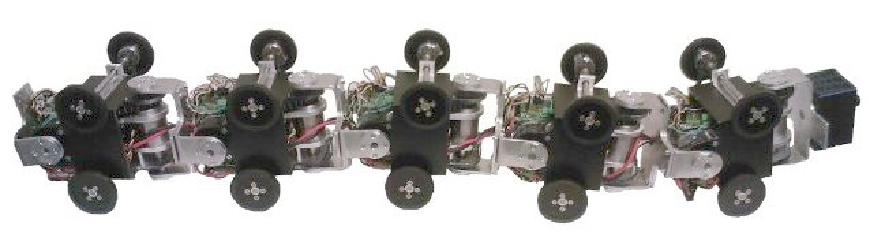
\includegraphics[width=0.8\textwidth]{pics/piko}
    \caption[The Pipe Inspection Konda]{The Pipe Inspection Konda. \url{www.sintef.no}}
    \label{chap1:fig-piko}
\end{figure}

Some of the key challenges when designing such a navigation system are the difficulties
with keeping track of where the robot is, and more importantly where it has been. This is
difficult in a pipe environment because it does not allow for a redundant positioning
system for global position estimation, such as GPS. The robot is then limited to using
either some kind of odometry or determination and tracking of landmarks in the environment, 
or both. The measurement noise will become an important factor when making the map,
because only small errors in the position or orientation will over time give large error
in the map when accumulated over time. \cite{thrun}

When the robot know where it is, it must take the decision on where it should go next. If
there is something blocking the way, it needs to handle these cases in some way.
Unfortunately, the world is not ideal as the usual lab environments and what to expect is
difficult to foresee. 
This calls for a robust system which can handle the situations that can
occur in the given mission environments. 

The report will define and select sensors applicable for a pipe inspection mission
preformed by the PIKo robot platform. The benefits and drawbacks of the different sensors
need to be assessed in detail. Next, the sensor data must be stored and interpreted in some
way, and important features that identify the position in the environment must be selected. 
This calls for processing of sensor data and an intelligent selection of the features that
will describe the environment in the best way. This is known as segmenting a data set.
When the dataset is divided into known geometric features, the estimation of the
parameters of these features can be done. 

PIKo is autonomous platform, and the computational abilities and memory available
are limited. The space available for the map representation is limited.
A map representation with little pre processing takes up much memory, while a
representation which processes the sensor output and estimates features need less space in
memory if the features are recognized by the system. 


\section{Assumptions}
As said above, this is a tremendous task to overcome in the time frame of this project. To
simplify and limit the task some assumptions are taken and summarized below. 
\begin{itemize}
    \item Only planar motion is assumed, even though the implementation platform is
    capable of vertical motion. 
    \item The environment which the robot will operate is structured. Most pipe
    environments are heavily structured. This allows for good prediction on what the robot
    might face in the mission. A good database can be created for what it will encounter. 
\end{itemize}

\section{Demands}
The complete navigation system for a pipe inspection robot should meet the following
demands and qualities. 
\begin{itemize}
    \item Robustness. The system should be robust and able to take the right decisions
    even when the sensors do not give good readings, at least for a limited time.
    \item Real-time system with limited computational abilities. The system is embedded
    and the processor power and memory available are limited. The algorithms should be
    efficient and the sensor data should be treated and stored in a memory efficient way. 
    \item Simplicity. Make thing as simple as possible but not simpler, a great scientist
    once said. This might help to keep the complexity of the system down. 
    \item Consistency. When faced with the same challenge over and over, the robot should
    take the same decision, over and over, because it will be the best one. The robots
    actions should be deterministic. 
    \item Modularity. The navigation system should be designed in a modular way, to allow
    for easy insertion of new features and functionality. 
\end{itemize}


\section{Structure of the Report}
The report is presented in the following way. Chapter \ref{chap2} give a thorough
introduction to the concepts needed to understand this report. It will address different
range finding techniques, and different sensor concepts will be introduced with advantages
and disadvantages of the concepts. Stereo imaging will be discussed in detail, from the
aspect of camera calibration and epipolar geometry to rectification of the captured images and
reprojection of the extracted disparity images. The most used map data representations will be
introduced and explained, also feature extraction and model fitting in Section
\ref{chap2:sec-representations} and \ref{chap2:sec-feature-extraction}. At last, a survey
of the different pipe inspection robots currently under research is included in Section
\ref{chap2:sec-state-of-the-art}.

Chapter \ref{chap3} concerns the selection of sensors appropriate for the application, and
calibration of those sensors. The lens distortion parameters and intrinsic parameters of the
sensors will be estimated and calibrated. 

A representation of the world will be proposed in Chapter \ref{chap5} together with how the sensor
outputs are interpreted.

Chapter \ref{chap6} and \ref{chap7} will deal with implementation and testing of the
proposed system, while Chapter \ref{chap8} will evaluate how the proposed system preformed
on the tests. The last chapter will give the main conclusions and propose further topics
for research. 



%included in thesis.tex,



\chapter{Background and Literature Study}
\label{chap2}
This chapter will try to outline the basics needed to understand this report. Mathematical
knowledge are crucial to understand the principles used in robot navigation and decision
making. The topics treated here include, general reference frames, homogeneous coordinate
representations, camera modeling, feature matching, map representations and optimization
criterions.



\section{Basics}

\subsection{Reference Frames}
	Movement must be described relative to something. This is the task of the reference systems. There are
	4 important reference system. The ECI (Earth Centre Inertial) which is a truly inertial reference
	frame, i.e. it is not accelerating. Its axis are pointing through the north pole and through the
	equatorial line of the Earth, fixed toward stationary points in space. The centre is as the name
	suggests in the centre of the Earth. 
	
	ECEF (Earth-Centre Earth-Fixed) is another reference frame. It is defined same as the ECI coordinate
	system, but the axis are rotating with the same rate as the Earths rotation rate. This means that this frame
	is not
	strictly inertial, but the angular velocity of the Earths rotation are considered very small, and can
	be neglected compared to other velocities in the same frame. Position on the earth are described by
	\emph{longitude} and \emph{latitude}.

	An important reference frame when considering local motion are the NED (North East Down) frame. This
	frame is defined as the tangent plane on the current position, and moving with the object. The axis
	are pointing towards north, east and down. This frame can be used in local, and small areas, but are
	not valid for intercontinental travel. This frame will primarily be used in this report. 

	The last but important frame are the Body frame, which is the local frame of the object of interest.
	The body frame are defined as the x-axis along its forward movement, y-axis to the right of the
	movement direction, and the last pointing downward, to complete the right-hand system. The
	origin are defined in the Centre of Gravity of the object. This frame are convenient when
	defining velocities, forces and moments. More on reference frames in \cite{fossen} and
    \cite{forsell}.
    \begin{figure}[htbp]
        \centering
       % \includegraphics[width=0.7\textwidth]{pics/referenceframse}
        \caption{The different reference frames in this report}
        \label{chap2:fig-ref-frames}
    \end{figure}

    The reference frames that will be considered in this report are the \emph{NED}- and
    \emph{body} frames. In addition to these two frames there are the last, but not least
    important frame, called the \emph{single-sensor} frame. This is where the output from
    the sensors are defined. These output need to be transformed into the \emph{body} and
    to the \emph{NED} frame to make sense for the control system and ultimately for the
    user. 

    The \emph{single-sensor} frames are where the individual sensors give readings. The
    exact mount point relative to the centre-of-gravity need to be defined, to make the
    transformation to other frames possible. The domain of the \emph{single-sensor} frames
    are defined in accordance to the domain of the sensor, i.e. the domain of a Laser
    Range Finder, which gives angles and ranges in the plane are two dimensional. 

    \begin{figure}[htbp]
        \centering
        %\includegraphics[width=0.7\textwidth]{pics/singlesensorframes}
        \caption{\emph{Single-Sensor} frames on PiKo}
        \label{chap2:fig-single-sensor-frames}
    \end{figure}


\subsection{Homogeneous Transformation Coordinates}
To represent transformations, i.e. rotations, translations, shear and scaling, it is
practical to represent those transformations in matrix form. But it is not mathematically
possible to represent both rotations and translations in the same matrix as long as it is
contained in $\mathbb{R}^3$. ******REFERENCE******

To overcome this problem, the coordinates are projected into a fourth dimensional space.
All points and vectors gain an extra element which describes if the coordinate is a vector
or a point. 
\begin{equation}
        \mathbf{v} = \left[ \begin{array}{c}
                                    x_v \\
                                    y_v \\
                                    z_v \\
                                    w_v  \end{array} \right]  =
                     \left[ \begin{array}{c}
                                    1 \\
                                    0 \\
                                    0 \\
                                    0  \end{array} \right] \quad \quad
        \mathbf{p} = \left[ \begin{array}{c}
                                    x_p \\
                                    y_p \\
                                    z_p \\
                                    w_p  \end{array} \right]  =
                     \left[ \begin{array}{c}
                                    1 \\
                                    0 \\
                                    0 \\
                                    1  \end{array} \right] \quad \quad
\end{equation}
Here $\mathbf{v}$ is a vector with the fourth element as zero, while $\mathbf{p}$ is a
point with the fourth element equal one.

This leads us to the \emph{Transformation Matrix} which is a $4 \times 4$ matrix. For
example a matrix representing rotation and translation will look like this
\begin{equation}
    \label{chap2:eq-TransformationMatrix}
    \mathbf{T_{rt}} = \left [ \begin{array}{cccc}
                                r_{xx} & r_{xy} & r_{xz} & t_x \\
                                r_{yx} & r_{yy} & r_{yz} & t_y \\
                                r_{zx} & r_{zy} & r_{zz} & t_z \\
                                0  & 0  & 0  & 1  \end{array} \right]
\end{equation}
Here the $r_{ii}$ coefficients are rotation parameters and the $t_i$ coefficients are the
translation parameters. The rotation coefficients are calculated from the Euler angles.

Likewise, scaling might be performed by the following transformation matrix
\begin{equation}
    \label{chap2:eq-TransformationMatrixScaling}
    \mathbf{T_S} = \left [ \begin{array}{cccc}
                                S_x & 0 & 0 & 0 \\
                                0 & S_y & 0 & 0 \\
                                0 & 0 & S_z & 0 \\
                                0 & 0 & 0 & 1 
                                 \end{array} \right]
\end{equation}
All of this transformations might be combined into a single matrix by multiplying the
matrices together, in the reverse of the order of which the transformations are carried
out. 


\section{Ranging Techniques}
The measure of distances and ranges are important and there are various ways of doing
this. Most techniques include the measure of time-of-flight of some signal and calculating
the distance from the known travel velocity of the signal. This requires the signal
emitted to be reflected, captured and processed at or close to the emitter. The signal is
usually electromagnetic or sound based, which allows for different kinds of modulations to
make the signal easier to recognize at the receiver.


This section will first outline the usual range determination techniques then go into the
more specific sensor characteristics in later sections.


\subsection{Triangulation}
The technique of triangulation is an old and well-known technique for range determination.
Two points with known locations are used. The distance between the two points are called
the \emph{baseline}. Instead of measuring the range to a third point directly the angles
from the two ends of the baseline to a third point is used to calculate the range
according to Equation \ref{chap2:eq-triangulation}. See Figure
\ref{chap2:fig-triangulation}.
\begin{equation}
    \label{chap2:eq-triangulation}
    d = b \frac{\sin{\alpha} \sin{\beta}}{\sin{\alpha + \beta}}
\end{equation}
\begin{figure}[htbp]
    \caption{Triangulation setup}
    \label{chap2:fig-triangulation}
\end{figure}

This technique is accurate for as long as all the points are in the same plane.


\subsection{Time-of-Flight Measurement}
This method of range determination is the most common, and utilizes the travel time of the
emitted signal. The signal might be in light, radio or sound waves. The precision of the
range greatly depend on the type of signal, the medium which it travels and the quality of
the time-measuring device. By knowing the velocity of the emitted signal and assuming it
is constant, the distance it travels can be determined with great accuracy according to 
Equation \eqref{chap2:eq-tof}
\begin{equation}
    \label{chap2:eq-tof}
    d = v \frac{t}{2}
\end{equation}



\section{Various Sensors Used in Robotics}
This section concerns the use of different kind of sensors in robotic applications. Only
sensors which are compliant to the overall perspective will be dealt with. This includes
laser range finders, ultrasound and Sonar sensors, Time-of-Flight cameras and
stereo cameras. 

\subsection{2D Sensors}

\subsubsection{Laser Range Finders}


When looking at Laser Range Finder, there are 3 techniques for determining the distance,
\emph{optical triangulation}, \emph{pulse Time-of-Flight} and \emph{frequency modulated
continuous wave} (FMCW). \cite{laser-ranging-critical-review}

\paragraph{Optical Triangulation}
Optical is very similar to triangulation described above and uses the same principle.
A light source are placed at the one end of the
baseline, and a light sensor at the other end which senses the reflected light from the
light source. The principle is basically the same as in normal triangulation. But, due to
the fact that a light source is used, and more closely a laser light source, the surface
that the laser light hits, the dot detected by the photo detector at the other end of the
baseline, needs to ''stay in focus``. If this is not done the laser dot will become a
blurred disc and the uncertainty to the point will become larger. To force the dot to
always be in focus, a special aligning of the lenses and photo detector are used, called 
the \emph{Scheimpflug} condition. The interested reader are referred to
\cite{laser-ranging-critical-review}.

The laser dot is contaminated with speckle noise which makes it more difficult to find the
exact center of the projected dot. This makes the determination of the along the third
dimension a bit more tricky, because of the positional uncertainty introduced by the
noise. Frequency of the light, angle and area of the collecting lenses and photo detector
are parameters that influence the position uncertainty. 


\paragraph{Pulsed Time-of-Flight}
The technique referred to as pulsed time-of-flight refers to the time taken of a pulse
train of laser light to be reflected back to the emitter. Light travels around 30 cm/ns,
this means that to get 1 mm accuracy the accuracy of the timing devices should be
6.7 ps.

Only a single laser pulse is necessary for the determination of the range with centimeter
precision this technique is suitable for fast measurements and range sweeps. If the
measurements are averaged millimeter precision might be acquired. 

The application and ranges that are going to be measured are dependant on what kind of
laser which is selected. The energy in the laser pulse effects the amplitude of the
reflected light and in turn affects the measurement accuracy.

Major sources of inaccuracies in a pulsed time-of-flight range finders are timing jitter,
nonlinearities, walk and drift. Jitter in timing is the source of precision errors in the
system. Precision also deteriorates as the distance increase and the reflected pulse
amplitude decrease proportional to the square of the distance\cite{pulsed-tof}.
Walk errors are due to shape variations in the pulse, which will create errors in the
timing measurement. 





\paragraph{Frequency Modulated Continuous Wave}
This technique have been used in in applications such as, surface profiling, tomography
reflectography and positioning. This is a technique which have large dynamic range and
high resolution at short range sensing. The principle is that a laser diode is applied
with a frequency periodically shifted by $\Delta f$. The signal is usually done with
applying a saw-tooth biased current to a wavelength-tunable laser diode. This saw-tooth
signal is also sent to be mixed with the reflected signal. The phase difference in the
reference signal and the reflected signal is $\tau = 2 R / c$ where $R$ is the range of
the traveled signal. The range is proportional to the intermediate frequency, i.e. the
frequency difference due to the travel time
\begin{equation}
    f_i = \Delta f \tau /t_m = 2 \Delta f R /c t_m
\end{equation}
$t_m$ is the ramp period of the saw-tooth signal. 

Both $\tau$ and $f_i$ can be measured, which one that is measured depends on the required
range and resolution. If the intermediate frequency is measured the resolution is best,
since the ramp time can be chosen freely, the need for high speed electronics are not
necessary, and a simple frequency counter in the kilohertz domain can be used to give the
sensor millimeter resolution.

Limitations of this technique is that the frequency characteristics of the laser diode is
seldom linear, which will result in a nonlinear reference signal, which leads to
variations in the intermediate frequency measurement.
\cite{laser-ranging-critical-review}.

\subsubsection{Sonar}


\subsubsection{Infrared Sensors and Proximity Sensors}


\subsection{3D Sensors}


\subsubsection{Time-of-Flight Cameras}
The research and application of Time-of-Flight cameras have increased significantly during the last four
years. A Time-of-Flight camera is a compact device which makes it suitable to mount on
mobile platforms, and thereby using it in navigation and localization applications. 

The most used ranging techniques by the cameras are \emph{intensity modulation} approaches and
\emph{optical shutter} technology. The first one is used by the best known manufacturers,
like MESA and PMD. While the optical shutter approach is less expensive and have been used
by Zcam, which now have been sold to Microsoft. 


\paragraph{Intensity Modulation Approach}
This approach uses modulated near infrared light (NIR), $g$ which is reflected to and
captured by a CCD chip then correlated with the reference signal, $r$. 
\begin{equation}
    c(\tau) = g \otimes r = \lim_{T \rightarrow \inf} \int^{T/2}_{-T/2} g(t) r(t + \tau) dt
\end{equation}
where the signals, $g$ and $r$ might be
\begin{equation}
    g(t) = \cos{\omega t}, \quad \quad r(t) = b + a \cos{(\omega t + \phi)}
\end{equation}
where $\phi$ is the phase offset because of the travel time of the signal, $b$ is a
correlation bias, $a$ is the amplitude and $\omega$ is the modulation frequency. Solving
the integral yields 
\begin{equation}
    c(\tau) = \frac{a}{2} \cos{(\omega \tau + \phi )} + b
\end{equation}
which is the correlation function. 

The demodulation is usually done by sampling the correlation function at 4 equally spaced
phase offsets. The following relation can now be written
\begin{equation}
    \begin{aligned}
        \phi &= \tan^{-1} (\frac{A_3 - A_1}{A_0 - A_2}) \\
        I &= \frac{A_0 + A_1 + A_2 + A_3}{4} \\
        a &= \frac{\sqrt{(A_3 - A_1)^2 + (A_0 - A_2)^2}}{2}
    \end{aligned}
\end{equation}
where $A_i = c(i \frac{\pi}{2})$ for $ i = 0,..,3$ and $I$ is the intensity of the returned NIR
signal. From this the distance can be calculated using the phase delay $\phi$. 
\begin{equation}
    d = \frac{c}{4 \pi \omega} \phi
\end{equation}

There are a number of challenges when using this approach
\cite{time-of-flight-comp-graphics}
\begin{itemize}
    \item The resolution of the sensors are small compared to standard RGB or grayscale
        sensors. Current resolution on present day time-of-flight cameras are $204 \times
        204$. 
    \item ``Wiggling'' because of imperfections when creating the sinusoidal signals.
    \item Errors due to intensity measurements. Various sensor electronics might influence
        the measured intensity and give wrong readings.
    \item ``Flying Pixels'' occurs when a pixel in the camera oversees a region with
        large depth variances, e.g. at object boundaries, because of superimposed signals. 
    \item Motion artifacts might occur because the phase images are captured sequentially
        quick motion might cause artifacts.
    \item Multiple reflections in highly reflective environments will cause erroneous
        distance measurements.
\end{itemize}

Standard lenses are used to capture the reflected light, which means that intrinsic
calibration should be carried out to specify the projection axis and distortion parameters
of the lens. See sections below for lens calibration and distortion coefficient
estimation. \cite{time-of-flight-comp-graphics}


\paragraph{Optical Shutter Approaches}
Light travels roughly at $c \approx 3 \times 10^8$ meters per seconds. This translates to
that light uses $7$ pico seconds to travel one millimeter. Imagine a light pulse emitted
at time $t$. This pulse travels in a spherical pattern and hits a 3D shape. The light wall
will be reflected back in a distorted pattern.\cite{optical-shutter} 
A shutter in front of the CCD chip then
shuts out the rest of the light wall pattern. This will then produce a shape of the object
which can be used to calculate the distance, based on the times the shutter is open,
according to the following relation \cite{time-of-flight-comp-graphics}
\begin{equation}
    d = (1 - \alpha) d_{min} + \alpha d_{max}, \quad \quad \alpha =
    \frac{I_{gate}}{I_{total}}
\end{equation}
where $I_{gate}$ is the pixel intensity which arrives when the shutter is open, and
$I_{total}$ is the total amount of reflected light. Distances outside $d_{min}$ and
$d_{max}$ cannot be measured in the exposure. Therefor this techniques require multiple
exposure to get the desired depth resolution. 

This method is also prone to the challenges stated for the intensity modulation approach
as well.

\paragraph{3D camera calibration}
This should outline how to calibrate the cameras. 



\subsubsection{Stereo Vision}
Stereo vision is an inexpensive way of finding range measurements. The setup is two or
more cameras some distance away from each other. This distance is called the
\emph{baseline}. The camera images are then compared and a common reference point is
found. The difference between the images are then used together with the baseline distance
to triangulate the common reference point and then find the distance to the observed
object. 

The process of Stereo Imaging involves 4 steps when using two cameras \cite{openCV}:
\begin{enumerate}
    \item Remove radial and tangential lens distortion caused by inexpensive lenses and
        image chips. This outputs \emph{undistorted} images. 
    \item \emph{Rectify} the images. This adjusts the angles and distances between the cameras.
        This outputs row-aligned images.
    \item Find the same features in the left and right camera view. This process is called
        finding \emph{stereo correspondences}. This outputs a \emph{disparity} map, which
        is the difference in x-coordinate of the feature in the left and the right image. 
    \item If the geometric configuration of the cameras are known, the disparity map can
        be translated into depth map with the help of \emph{triangulation}. This final
        step is called \emph{reprojection}.
\end{enumerate}
This steps will be described in detail below. 


\paragraph{Pinhole Camera Model}
A camera model is needed to understand how light is captured on the image plane. To do
this a \emph{pinhole camera} model is used to capture light form a point. This model
assumes that only one light ray from each point travels trough a infinite small hole in
a plane, called the \emph{focal} plane and hits a second plane, called \emph{image} plane.
These two planes are placed a distance, $f$ from each other. Using elemental geometry the
coordinates of the real world point imaged at the image plane can be calculated. 
\begin{equation}
    -x_i = f \frac{X}{Z}
\end{equation}
where
\begin{equation}
    P_i = \left [ \begin{array}{c}
        x_i \\
        y_i 
    \end{array} \right]  \in \mathbb{R}^2 \quad \quad P_w = \left [
    \begin{array}{c}
        X \\
        Y \\
        Z \\ 
    \end{array} \right] \in \mathbb{R}^3 
\end{equation}
\begin{figure}[hbtp]
    \centering
    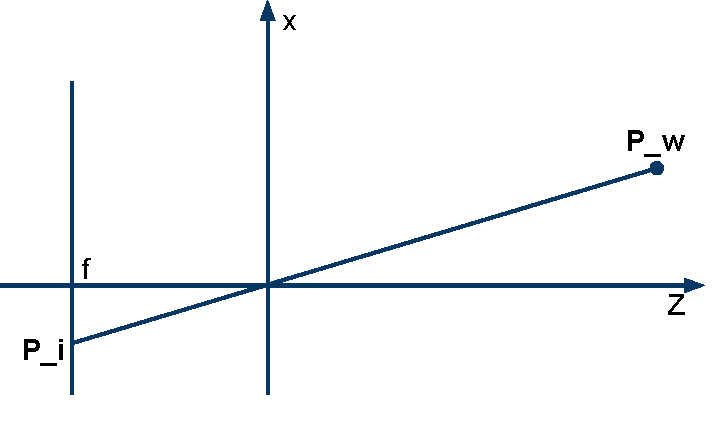
\includegraphics[width=0.7\textwidth]{pics/pinhole_model}
    \caption{Pinhole Camera Model showing two dimensions}
    \label{fig:ch2-pinhole}
\end{figure}

Figure \ref{chap2:fig-pinhole} shows the configuration with the pinhole located at
Origo and the image plane located at $f$. Where the pinhole is are often termed
\emph{center of projection}. The x axis of the image is located
upwards, while the real Z axis are the horizontal axis, that are called the
\emph{optcal axis}. This lead us to the next parameters which need to be defined.

The optical axis should ideally always be aligned with the center of projection. Due to
manufacturing inaccuracies this is rarely the case, therefor we need two more parameters
in to complete the pinhole model equations. This parameters are $c_x$ and $c_y$ which
describes the offset of the optical axis from the center of projection. Also the need for
different focal lengths in $x$ and $y$ might also be a necessity, because the individual
pixels on a typical low-cost image chip is rectangular rather than square. Now the
equations relating real-world coordinates to image coordinates can be written.
\cite{openCV}
\begin{equation}
    x_i = f_x \frac{X}{Z} + c_x \quad \quad y_i = f_y \frac{Y}{Z} + c_y
\end{equation}

The equations above are the \emph{projective} transformations, and are convenient to
write using homogeneous coordinates and arrange the parameters into a single $3\times 3$
matrix. This matrix is sometimes called the \emph{camera intrinsic} matrix. 

\paragraph{Lens Distortion}
\label{chap2:sec-distortion}
Because very little light goes through the pinhole, and to make the camera practical for
real world use, lenses are used to bend, i.e. focus more light to the projective plane.
This allows for faster imaging of the world, but is also the source of more distortions
and inaccuracies. 

There are two types of lens distortions, \emph{radial} and \emph{tangential}. Radial
distortions are due to the lens construction. Most distortion occurs towards the edges of
the lens. This can be seen in pictures as ``barrel'' or ``fish-eye'' effects. These
effects are more present in cheap cameras which does not have the fancy lenses and optics
that the more high-end cameras have. There is also other types of distortions in imaging
systems, but they have typical lesser effects on the images, and will not be taken into
account. 

To model radial lens distortions the approach described by Brown in
\cite{lens-calibration} are used. The radial distortion are in practice small and can be
described by the two first terms of a Taylor series expansion around the center of the
lens. If the lens have high radial distortion, like fish-eye lenses a third term are
appended. The radial location of the point on the image plane can in general be described
like the equations below. 
\begin{equation}
\begin{aligned}
    x_{corrected} &= x_i ( 1 + k_1 r^2 + k_2 r^4 + k_3 r^6 ) \\
    y_{corrected} &= y_i ( 1 + k_1 r^2 + k_2 r^4 + k_3 r^6 ) 
\end{aligned}
\end{equation}

Tangential distortion is due to manufacturing defects which causes the lens not to be
perfectly parallel to the imaging plane. This causes the image to become more like a
trapezoid. This can be modeled by equations \eqref{chap2:eq-tangential-distortion}. The
derivation of this equations can be found in \cite{brown66}.
\begin{equation}
    \label{chap2:eq-tangential-distortion}
    \begin{aligned}
        x_{corrected} &= x_i + (2 p_1 y_i + p_2 (r^2 + 2 x_i^2)) \\
        y_{corrected} &= y_i + ( p_1 (r^2 + 2 y_i^2) + 2 p_2 x_i))
    \end{aligned}
\end{equation}
The parameters $p_1$ and $p_2$ are the tangential distortion parameters. This parameters
gives enough information about the lens and camera to make corrections to the picture and
make the matching method easier and the measurements more accurate. This calibrations will
be shown in Chapter \ref{chap3-sensors} for the selected stereo cameras. 


\paragraph{Epipolar Geometry}
To describe the stereo rig and geometry between the left and right cameras, the term
\emph{epipolar geometry} is introduced. Epipolar geometry exists between any two cameras.
The different center of projections, $O_r$ and $O_l$, and corresponding
projective planes, $\Pi_r$ and $\Pi_l$ and the term \emph{epipole} on the projective plane
$\Pi_r$, $e_r$ can now be defined as the image of the center of projection of the other 
camera, $O_l$. Suppose the point, $P$ are viewed from both cameras, and have the image
location, $p_l$ and $p_r$ in the left and right view, respectively. The line from the left
epipole, $e_l$ to $p_l$ and the line from $e_r$ to $p_r$ are called the \emph{epipolar
lines}. The planes made by the observed real world point, $P$ and the center of
projections, $O_r$ and $O_l$ are called the \emph{epipolar planes}. See Figure
\ref{chap2:fig-epipolarGeometry}
\begin{figure}[htbp]
    \centering
    %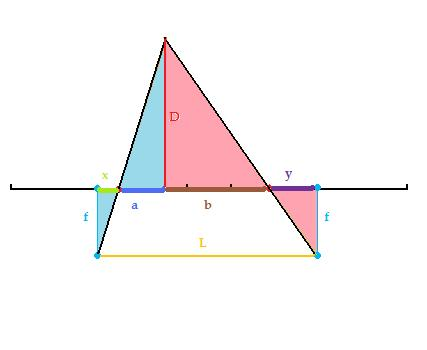
\includegraphics[width=0.5\textwidth]{pics/stereo_geometry}
    \caption{The epipolar geometry}
    \label{chap2:fig-epipolarGeometry}
\end{figure}

This allows for the following facts which simplifies the computations a great deal.
\cite{epipolar}
\begin{itemize}
    \item Every 3D point in view of the cameras is constrained in an epipolar plane that
        intersects each image in an epipolar line.
    \item The \emph{epipolar constraint} says that a given feature in one image must lie
        along the corresponding epipolar line in the other view.
    \item The epipolar constraint means that the two-dimensional search for matching
        features simplifies to a one-dimensional search along the epipolar lines once the
        epipolar geometry of the stereo rig is known.
    \item The order is preserved. If two points are visible in both images and occur
        horizontally in that order in one image, they occur in the same order in the other
        image.
\end{itemize}

\paragraph{The Essential and Fundamental Matrices}
This matrices contains information about the translation and rotation which relate the
two cameras. The Essential matrix describes this translation and rotation in physical
space, while the Fundamental matrix also contains information about the intrinsics of the
two cameras, thereby describing the rotations and translations in pixel related
coordinates.

The derivation of the Essential matrix is interesting and is given here for reference.
Suppose a point $P$ related in the left camera coordinates, i.e. $P_l$ and the right
camera is located at $T$. The coordinates of $P_l$ in the right camera coordinates will
then be.
\begin{equation}
    \label{chap2:eq-Pr}
    P_r = R (P_l - T)
\end{equation}
Now, the epipolar plane is introduced. All points, $\mathbf{x}$ that lay on the plane with normal vector
$\mathbf{n}$ and passing through $\mathbf{a}$ obeys the equation,
\begin{equation*}
    (\mathbf{x} - \mathbf{a}) \cdot \mathbf{n} = 0
\end{equation*}
The cross product of $T$ and $P_l$ then becomes the normal vector of the epipolar plane,
because the epipolar plane includes both this vectors. Equation \eqref{chap2:eq-Pr} can be
rewritten as $P_l - T = R^{-1} P_r$ and including the cross product yields 
\begin{equation}
    (R^{-1} P_r)^T (T \times P_l) = 0
\end{equation}
The cross product can be expressed as a product between matrices by introducing the
skew-symmetric matrix $S$. \cite{modsim}
\begin{equation}
    S = \left [ \begin{array}{ccc}
                0 & -T_z & T_y \\
                T_z & 0 & -T_x \\
                -T_y & T_x & 0 \\ \end{array} \right]
\end{equation}
The essential matrix might now be defined with $R^{-1} = R^T$ and moving it behind $P_r$.
\begin{equation}
    E = RS 
\end{equation}
which gives the equation
\begin{equation}
    \label{chap2:eq-fundamental}
    P_r^T E P_l = 0
\end{equation}
$P_r$ and $P_l$ are the real world 3D coordinates, and can be transformed to 2D
coordinates by the perspective transformation derived by the pinhole camera model. 

The relation between the Essential matrix and the Fundamental matrix can be showed with
help of the camera intrinsic matrix $M$, because we know that $q = Mp$, where $q$ are
pixel coordinates and $p$ are the 2D world coordinates. Substituting for $P$ in Eqauation
\eqref{chap2:eq-fundamental} gives: \cite{openCV}
\begin{equation}
    q_r^T(M_r^{-1})^T E M_l^{-1} q_l = 0
\end{equation}
The definition of the fundamental matrix, $F$ is then
\begin{equation}
    F = (M_r^{-1})^T E M_l^{-1}
\end{equation}
Both matrices are $3\times3$ and have rank two with seven parameters.


\paragraph{Finding Stereo Correspondences}
Now that the mathematics which describes points in the different views to each other, the
case of matching the same points together can begin. This is obviously only possible for
visual areas that the two camera views overlap. 

There are couple of different matching algorithms. The most common are \emph{block
matching} algorithms. In \cite{konolige} a practical implementation of the block
matching algorithm are described. This algorithms use sum of absolute difference (SAD) windows to match same
same points in the two views. This algorithm work only on undistorted, rectified stereo
images. It first normalizes the image brightness which enhances textures. Then the search
for correspondences are carried out along the horizontal epipolar lines using the sum of
absolute difference window. After this the results are filtered to eliminate bad stereo
matches. This algorithm works best in highly textured environments, like outdoor
environments, and will prove less effective in structured surroundings like office
corridors and inside smooth pipelines. 

Another common matching algorithm are \emph{graph cut} algorithms. 

An extensive review of the different matching algorithms and their computational costs
can be seen in \cite{stereo-algorithms}.


\paragraph{Disparity and depth calculations}
When finally the stereo correspondences are found, the \emph{disparity} can be calculated.
The disparity is the difference in pixels coordinates from of the matched feature from one
image to the other. This disparity is inversely proportional to the depth. This means that
the depth perception of the stereo rig is better when relatively close to the cameras, as
Figure \ref{chap2:fig-disparity-depth} shows.
\begin{figure}[htbp]
    \centering
    %\includegraphics[width=0.5\textwidth]{pics/disparity-depth}
    \caption{The relationship between depth and disparity}
    \label{chap2:fig-disparity-depth}
\end{figure}

Many robotic applications using stereo cameras utilizes the disparity maps directly,
because they usually just require the detection of obstacles. ****REFERENCES ON THIS****

The 3D coordinates of the point can be calculated form the disparities given by the
matching algorithms. This is the process of \emph{reprojection}. Using triangulation
between the two known camera locations the depth can be derived accordingly to 
\begin{equation}
    D = f (T / d - 1)
\end{equation}

\begin{figure}[htbp]
    \centering
    %\includegraphics[width=0.5\textwidth]{pics/stereo-triangulation}
    \caption{Triangulation in the stereo rig}
    \label{chap2:fig-stereo-triangulation}
\end{figure}




\section{Map Data Representation}
The representation of sensor data is important for the functionality of the robot. This is
dependant on the amount of processing power and capacity that is available at the robot.
The area which the robot is to map is also of great importance when choosing the
representation. There are a number of representations that are tried out, and each one has its good and
bad abilities. 

The major representation methods which is used in literature are summarized in the below
sections. There are two major ideas when it comes to map representation, and that is
metric and topological.

Metric representation uses the sensor data as we see it. It is the direct Cartesian
representation of the way the world is. Examples of this are CAD drawings of floor plans
and housing. This maps are often large and inexact, because of many kinds of
uncertainties.

Topological representations uses a more abstract way. The world are represented by graphs,
which is nodes and links between them. This are a sparse and efficient way of representing
the world, but need more processing when the map is built. This kind of maps are not
exact, because they are not expected to be. They simply describe the connection between
different kind of objects, and all objects might have attributes describing how it really
looks. This method is useful in highly structured environments, such as pipelines, sewers,
and office landscapes. This because a series of junctions might tell you where you are
than just the metric information, which might be quite erroneous. 


\subsection{Occupancy Grid Maps}
Occupancy grid maps are a metric approach to the mapping problem and are widely used in 
robotic mapping, mostly because of it is simple to implement and use. It was developed 
by Elfes and Moravec in the mid 1980s, \cite{elfes}, \cite{moravec}. The method is quite 
robust and it is simple to implement with many kinds of sensors. This method assumes that 
the robots pose is known.

This method divides the world into grids with probabilities that the grid is occupied. It
starts with all grids at 50 \%, equal probability that the space is occupied or not. As
the robot moves around it updates the grids according to its sensor readings. When for
example employing laser range finders, the grid at the distance reported from the range
finder are marked as occupied according to some uncertainty set by the accuracy of the
range finder. The grids between the possible detected obstacle will then be decreased
because the probability of obstacles are less. 

Occupancy maps are not the most computationally effective way to represent the world,
especially when it is big. It is cumbersome and may lead to problems when dealing with
cyclic environments. This because of the uncertainty in the sensor measurements and robots
pose and odometry. 


\subsection{Quad- and Oct-trees}
Quadtrees can be used to represent a 2D space by recursively dividing the space into
exactly four rectangles or squares. If this rectangles or squares does not include
interesting information then it will not be divided further. This dividing continues until
the smallest possible square is achieved. This creates a tree structure which is easily
traversed and searched if necessary. 

\begin{figure}[htbp]
    \centering
   %\includegraphics[width=0.5\textwidth]{pics/quad-tree}
    \caption{A Quadtree representation}
    \label{chap2:fig-quadtree}
\end{figure}


\subsection{Topological Maps}
Object maps are topological maps and represents the sensed world in the form of predefined nodes and links
between them. Each node has a set of attributes, like length, links to doors etc. This is
a compact way to express the world and is much more computationally effective with larger
maps than the occupancy grid maps might be. Examples of such nodes are corridors,
junctions and dead ends, but this nodes must be suited to the application of the robot. 

The problem with this representation is that it needs a lot of input \'a priori. The
operator creates and inputs the map to the robot, which uses this map for navigation. The
largest challenge with this is to make the robot aware of where it is. It needs in some
way to recognize its surroundings, and match it to the \'a priori map.


\subsection{Mixed Approaches}
This is when you take the best of both worlds. The easy and effective way of the metric
maps, and mix them with the abstract topological maps. This will help reduce the size of
the maps in the robots memory, and also make it more computationally effective because the
maps are sparse. 

******?????The mixed approaches are usually not computed on-line***???? (CHECK THIS). This utilizes
the metric approach for the rooms that have a lot of details, chairs, desks etc. and for
corridors and less detailed areas the topological approach, when the metric and
geographical information are not that important. 

This requires lots of processing of the sensor and map data, and should be done off-line
after the robot's mission is finished. 


\section{Sensor Fusion Techniques}
According to \cite{sensor-fusion-mobile-robots} theres a lot of ways to achieve sensor
fusion in mobile robotics. The use of multiple sensors are favorable because the readings
can be fused to make a better estimate of the current situation. 

Multi sensor fusion are widely used in robotics today. This because it allows the designer
to use different measurement principles which have different capabilities. 


\begin{itemize}
    \item Low-level Fusion with unknown statistics
        \begin{itemize}
            \item Rule-based
            \item Geometric and topological maps
        \end{itemize}
    \item Low-level Fusion with known statistics in centralized approaches
        \begin{itemize}
            \item Kalman Filter and probabilistic approaches
        \end{itemize}
    \item Low-level fusion with known statistics in decentralized architectures
        \begin{itemize}
            \item Decentralized probabilistic approaches
        \end{itemize}
    \item High-level Fusion
        \begin{itemize}
            \item Behaviour-based architectures
        \end{itemize}
\end{itemize}


\subsection{Low-level Fusion}
The term low-level fusion is often used when the sensor data is directly integrated
resulting in parameters and state estimates of the model. This methods are mostly purely
mathematical. This method involves the Kalman Filter, and other Bayesian approaches. In
many cases the use of \'a priori information are utilized to verify or improve the
estimates from the sensors.

This methods are probabilistic and requires that you know something about the
statistical properties of the sensors and the \'a priori model. 


\subsection{High-level Fusion}



\subsection{Interpolation Techniques}



\subsection{Probabilistic Techniques}



\section{Feature Extraction}
The need for feature extraction should be obvious when dealing with autonomous robot
navigation. For the robot to know where it is it needs to recognize its surroundings. This
is a difficult step, because computers are not known to be very good at this, as the human
brain is. 

By feature extraction it is meant to recognize one point or feature in one instant and
find the same point at the next time instant. This can be imagined difficult in some
surroundings where theres little individual detail. 

This problem is relaxed a bit when the surroundings are confined to pipelines. The problem
here is that the interior of the pipeline are not rich in detail, and is mostly the same
everywhere the robot travels, except in the different kinds of junctions. By feature
extraction in this report the meaning is to recognize the different types of junctions
that the robot will travel through. 
\cite{theilemann-breivik}



\subsection{Surface Fit Algorithms}


\subsubsection{Leasts-Squares Gauss-Newton Optimization}
Least-squares method is a common way to optimize and fit data sets to a proposed model.
The idea is to minimize the objective function 
\begin{equation}
    f(x) = \frac{1}{2} \sum_{j = 1}^m r^2_j (x)
\end{equation}
where the $r_j(x) \in \mathbb{R}^n \rightarrow \mathbb{R}$ is called the \emph{residual} and
is generally a linear or nonlinear function. This function can be written as a vector then
the Jacobian can be defined as
\begin{equation}
    J (x) = \left[ \frac{\partial r_j}{\partial x_i} \right]
\end{equation}
The Jacobian is a $m \times n$-matrix. Using this the Hessian, i.e. the second order
derivative of $f$ can be expressed as
\begin{align}
    \nabla f(x) &= \sum_{j = 1}^m r_j(x) \nabla r_j(x) = J(x)^T r(x) \\
    \nabla^2 f(x) &= \sum_{j=1}^m \nabla r_j (x) \nabla r_j(x)Å T + \sum_{j=0}^m r_j(x)
    \nabla^2 r_j(x) = J(x)^T J(x) + \sum_{j= 0}^m r_j(x) \nabla^2 r_j(x)
\end{align}
This allows for that the Hessian, which usually is very cumbersome and computationally
intensive to calculate can be approximated by the Jacobian. This is especially true when
the residual terms are small.

The Gauss-Newton method uses is a modified Newton method that uses line search to find the
best fit. Standard Newton methods are based on solving $\nabla^2 f(x_k) p = -\nabla
f(x_k)$ with regard to $p$ to find the search direction. The Gauss-Newton approach uses
the approximation $\nabla^2 f_k \approx  J_k^T J_k$, which gives the following equation to
solve
\begin{equation}
    J_k^T J_k p_k = - J_k^T r_k
\end{equation}


\subsubsection{RANSAC Algorithm}


\subsubsection{M-SAC Criterion}



\section{Real World Applications}

Remember MAKRO! The German snake robot used for sewer inspections. 






%file included in thesis.tex


\chapter{Sensors}
\label{chap3-sensors}
The sensors of a autonomous system is one of the key components for the application to
succeed. The sensors are eyes, ears and touch for the robot, and for the robot to be able
to complete its mission in a favourable way, the right sensors must be chosen.

The main sensor suit of the PiKo platform with regard to the pipe inspection and
navigation will be a 2D laser range finder, a Time-of-flight camera and a stereo camera
rig. The other sensors involved on the PiKo platform is beyond the scope of this report
and will not be investigated. 

Some common laser range finders will be compared and one will be selected. The stereo
camera rig are calibrated and both extrinsic, intrinsic parameters and distortion
coefficients will be determined. The time-of-flight camera are also calibrated for lens
distortions and intrinsic parameters will be determined. The different error sources associated
with the senors will also be mentioned.

\section{Comparisons Between the Proposed Sensors}
For this project, some of the sensors was not decided. This gave the ability to chose a
sensor, based on cost, resolution, accuracy and delivery date. The manufacturers that were
considered where the Japanese \emph{Hokuyo} and American \emph{SICK}. This two companies are to the
authors knowledge the leading manufacturers of laser range finders, small enough to be
mounted on small robotic platforms. The various models and key parameters are summarized
in Table \ref{chap3:tab-sensors}.
\begin{table}[htbp]
    \begin{tabular}{|c|c|c|c|c|c|}
        \hline
        Sensor              & LMS-100 & UTM-30LX & URG-04LX & URG-04LX-URG01 \\
        \hline
        Max Range           & 20 m    & 30 m     & 4 m      & 5.6 m          \\
        Accuracy            & 12 mm   & 30 mm    & 10 mm    & 30 mm          \\
        Field-of-View       & $270^\circ$& $270^\circ$ & $240^\circ$ & $240^\circ$  \\
        Angular Resolution  & $0.25-0.5^\circ$  & $0.25^\circ$ & $0.36^\circ$ & $0.36^\circ$  \\
        Scan Frequency      & 50 Hz   &  40 Hz   & 10 Hz    & 10 Hz          \\
        Weight              & 1.1 Kg  &  210 g    & 160 g    & 160 g          \\
        Power Consumption   & Not Specified  & $<8 $ W & $~2.5$W  &$~2.5$W  \\
        \hline
        Cost                & \$5500  & \$5000   & \$2400   & \$1100         \\
        \hline
    \end{tabular}
    \caption{Comparison between the proposed sensors}
    \label{chap3:tab-sensors}
\end{table}

The LMS-100 and LMS-200(not shown in the table) are relatively large sensors compared to
the ones from Hokuyo. The LMS-200 have been thoroughly tested and used in robotic
applications for a long time. The LMS-100 is a newer sensor, and is much smaller than the
LMS-200 \cite{SICKweb}. The advantage of the SICK laser scanners are their scanning
frequency, which is very fast compared to the Hokuyo laser range finders.

The criteria for sensor selection are:
\begin{itemize}
    \item Accuracy
    \item Price
    \item Size
    \item Power consumption
    \item Time of delivery
\end{itemize}
Because of favourable size, weight, accuracy and cost the Hokuyo \emph{URG-04LX} was
chosen. The sensor will be discussed in Section \ref{chap3:sec-urg}.

\subsection{3D Sensors}
There are many different depth sensors available at the consumer market. This section will
outline some of them, and describe the \emph{MESA Imagining} SR-3000 in more detail.
The development of depth-sensing cameras and devices have accelerated the last years
because of the increased computational ability and the fact that electronics become
cheaper and cheaper. \cite{low-cost-depthcameras}

During the next years the video game industry most certainly will
incorporate this new technology into video games to take the games to a new level, such as
Microsofts \emph{Project Natal} for Xbox 360 \cite{project-natal}. This uses infrared
projected light stereo. The camera will sense depth by using stereo cameras to sense a
coded near-infrared light pattern, by using standard CMOS image sensors. According to
Microsoft the accuracy in depth will be about 1 cm, and practical ranges will be about
1 to 3.5 meters. The camera will operate at 640x480 pixel resolution at 60 Hz
\cite{conceivably-tech}.



\section{Laser Range Finder Hokuyo URG-04LX}
\label{chap3:sec-urg}
The laser range finder which were selected to this application was the \emph{Hokuyo
URG-04X}. It uses an infrared laser to sweep a view field of $240^\circ$ ten times a
second. The full $360^\circ$ circle are segmented using ten bit, which gives angular
resolution of $\frac{360}{2^{10}} = 0.3515$. The ranges have twelve bit resolution, each
bit representing a millimeter, which gives the total measurable length of $2^{12} = 4096$.
\begin{figure}[htbp]
    \centering
    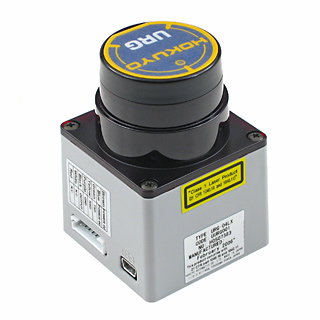
\includegraphics[width=0.4\textwidth]{pics/urg04lx}
    \caption{The Hokuyo URG-04X. \url{http://www.hokuyo.com}}
    \label{chap3:fig-urg}
\end{figure}
The effective area which gives range readings are the sector form the 44th step to
725th step. See Figure \ref{chap3:fig-urg-sector}. If $0^\circ$ is straight ahead, then
the measurement starts at $-135^\circ$ and stops at $135^\circ$. 
\begin{figure}[htbp]
    \centering
    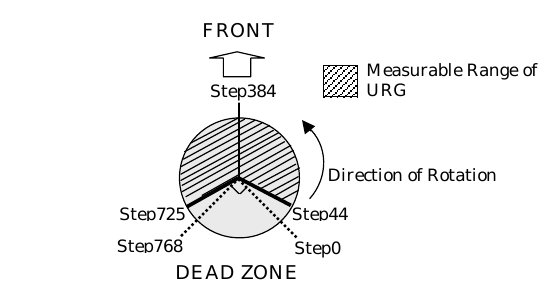
\includegraphics[width=0.7\textwidth]{pics/urg-sector}
    \caption{The sweep sector of the URG-04X}
    \label{chap3:fig-urg-sector}
\end{figure}

The sensor can not measure below 20 mm because it is not practical, and the range codes
from 0--19 are error codes. The codes can describe if the intensity of the reflected light
is too low or too high which indicates erroneous results. A detailed summary of the
error codes and what they mean can be found in Appendix \ref{app:urg-error}.


\subsection{Noise- and Error Sources}
Major error sources of laser range finders where discussed in Section \ref{chap2:subsec-lrf}. It is
possible to read both range and intensity of the reflected signal from the URG. The
intensity can be used as a quality control of the range value. Beyond this, no error
detection or redundancy are used. 



\section{Stereo Camera Minoru 3D WebCam}
The stereo camera chosen for the project is the first commercially available 3D Webcam.
\begin{figure}[htbp]
    \centering
    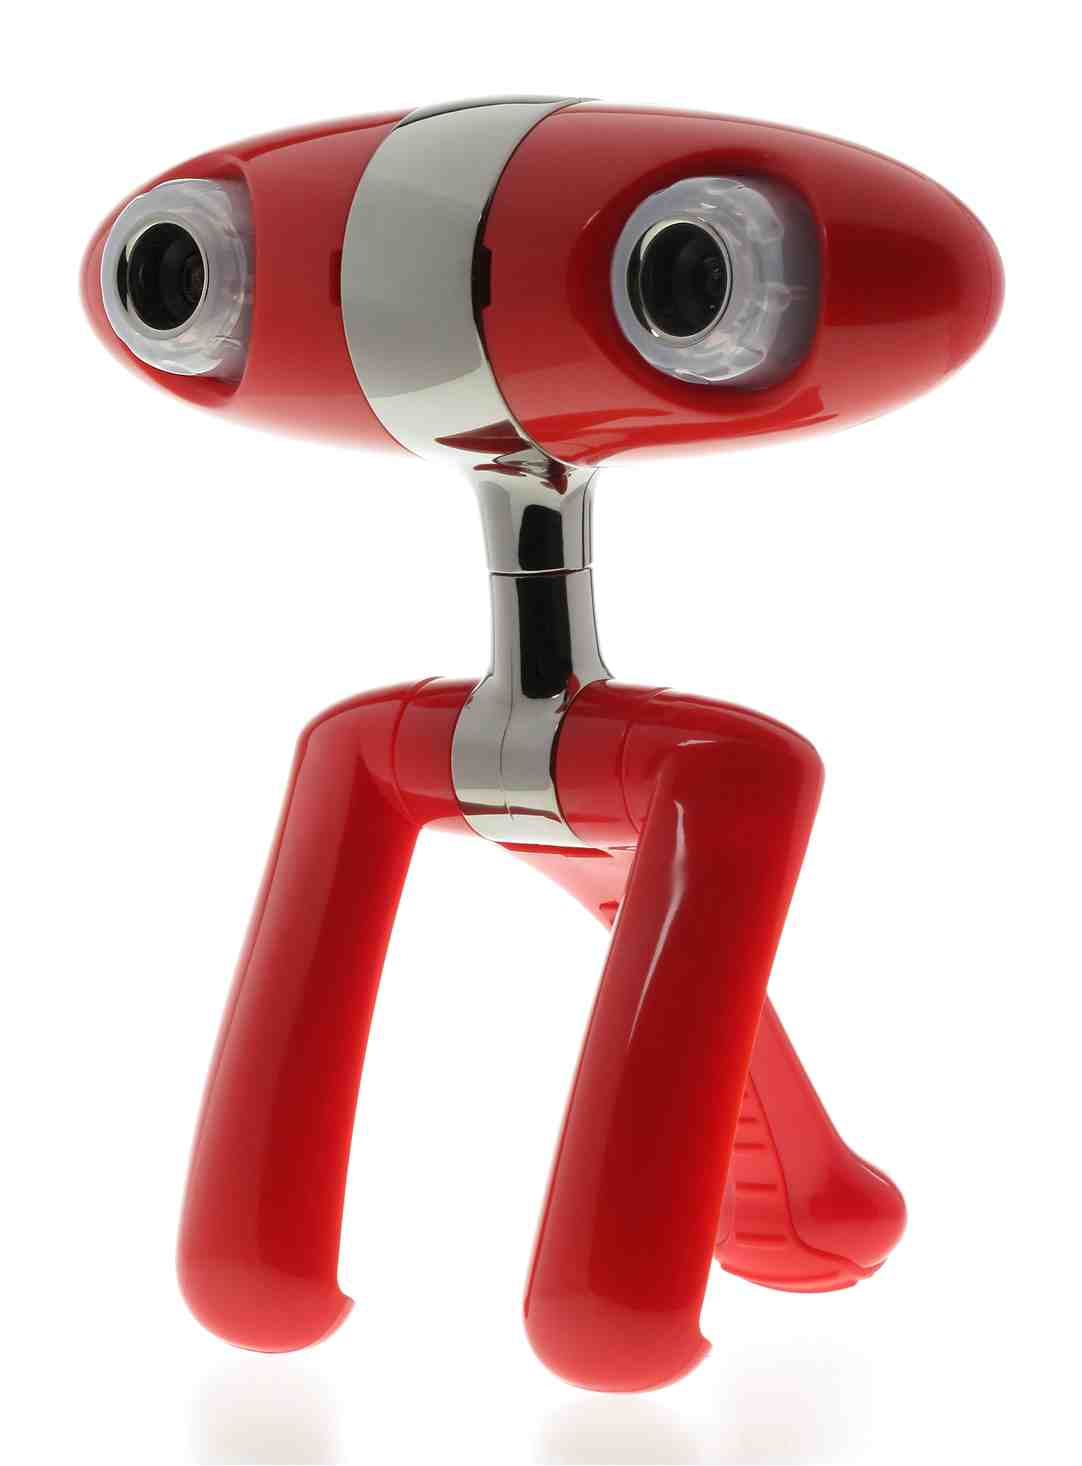
\includegraphics[width=0.35\textwidth]{pics/minoru3d}
    \caption{The Minoru 3D WebCam. \url{www.minoru3d.com}}
    \label{chap3:fig-minoru}
\end{figure}
It is actually just two cheap webcams and a USB hub in the same casing. The camera is
available for about 900 NOK, so both optics and imaging chips are expected to be of poor
quality. Also, the left and right camera shutters does not synchronize, \cite{nma-web}
suggests it might be as much as 16.5 milliseconds which might cause problems in fast
moving environments. 


\subsection{Camera Calibration}
To work with stereo images the captured images need to be rectified, i.e. the images need
to be corrected for distortion introduced by the camera lenses. This is a part of
calibrating the camera, meaning that the intrinsic parameters of the camera are
determined and the lens distortion parameters described in Chapter \ref{chap2}.

To determine the parameters the \emph{Camera Calibration Toolbox} for Matlab is used
\cite{camera-calib-toolbox}. 20 image pairs are captured of a checker board in various
distances and orientation from the stereo rig. This images for left and right camera are
processed individually to calculate the distortions of the individual camera. 
\begin{figure}[htbp]
    \centering
    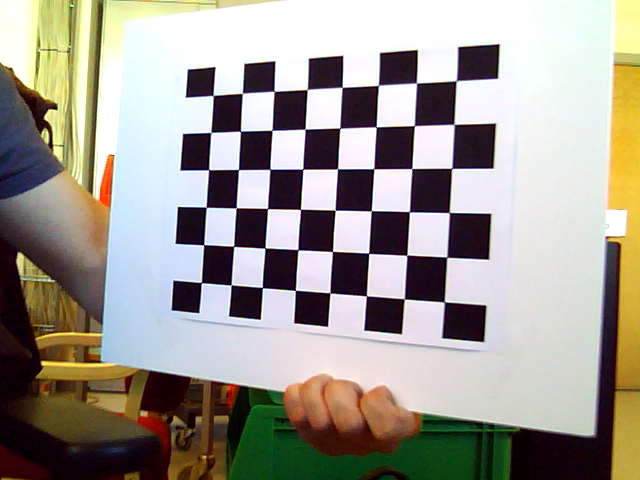
\includegraphics[width=0.8\textwidth]{pics/left7}
    \caption{Seventh left image in the calibration sequence}
    \label{chap2:fig-checkerboard}
\end{figure}
The four extreme-most corners of the checkerboard is selected in each image, and an
internal algorithm detects the corners of the squares in each image. This gives an initial
guess on how the distortion parameters are. The reprojection error is then minimized with
regard to the distortion parameters using a nonlinear gradient decent algorithm. For more
information on how this is carried out, see \cite{heikkila}.
The distortion parameters for both cameras are summarized in Table
\ref{chap3:tab-distortion-coeffs}.
\begin{table}[htbp]
  \centering
    \begin{tabular}{|c|c|c|} 
        \hline
                & Left Camera       & Right Camera \\
        \hline
        $k_1$   & $-0.10292 \pm 0.3794$            & $-0.5450 \pm 0.02456$  \\
        $k_2$   & $-0.22555 \pm 0.49387$            & $-0.38334 \pm 0.13037$  \\
        $h_3$   & $ 0$                          & $0$                  \\
        \hline
        $p_1$   & $-0.00361 \pm 0.00141$    & $-0.00033 \pm 0.00115$ \\
        $p_2$   & $0.00206 \pm 0.00174$     & $ 0.000491 \pm 0.00243$  \\
        \hline
    \end{tabular}
    \caption{The distortion parameters discussed in Section \ref{chap2:sec-distortion}}
    \label{chap3:tab-distortion-coeffs}
\end{table}

Figure \ref{chap3:fig-comp-lensdist} below shows how the camera lenses of the Stereo camera distorts the pictures
towards the edges of the lens. 
\begin{figure}[htbp]
    \centering
    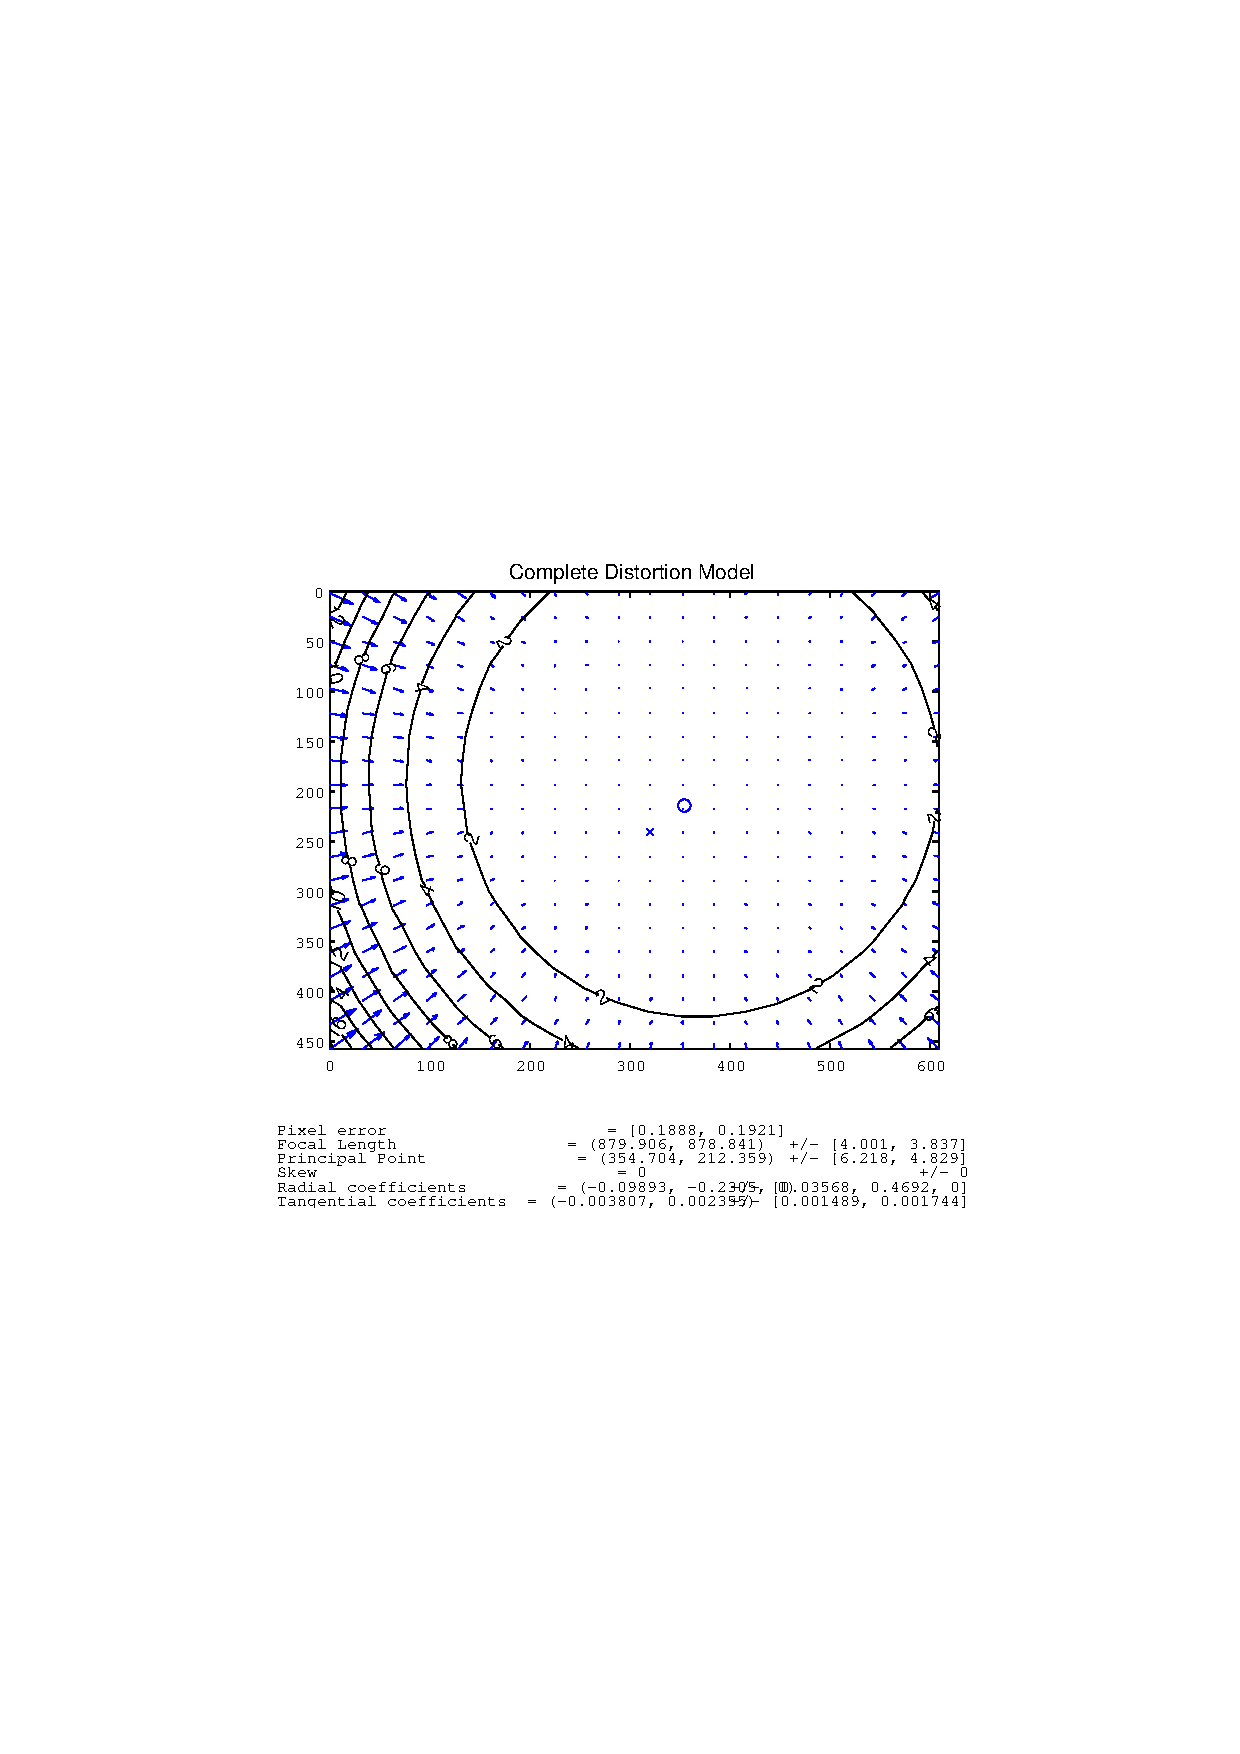
\includegraphics[width=0.47\textwidth]{pics/left_comp_dist}
    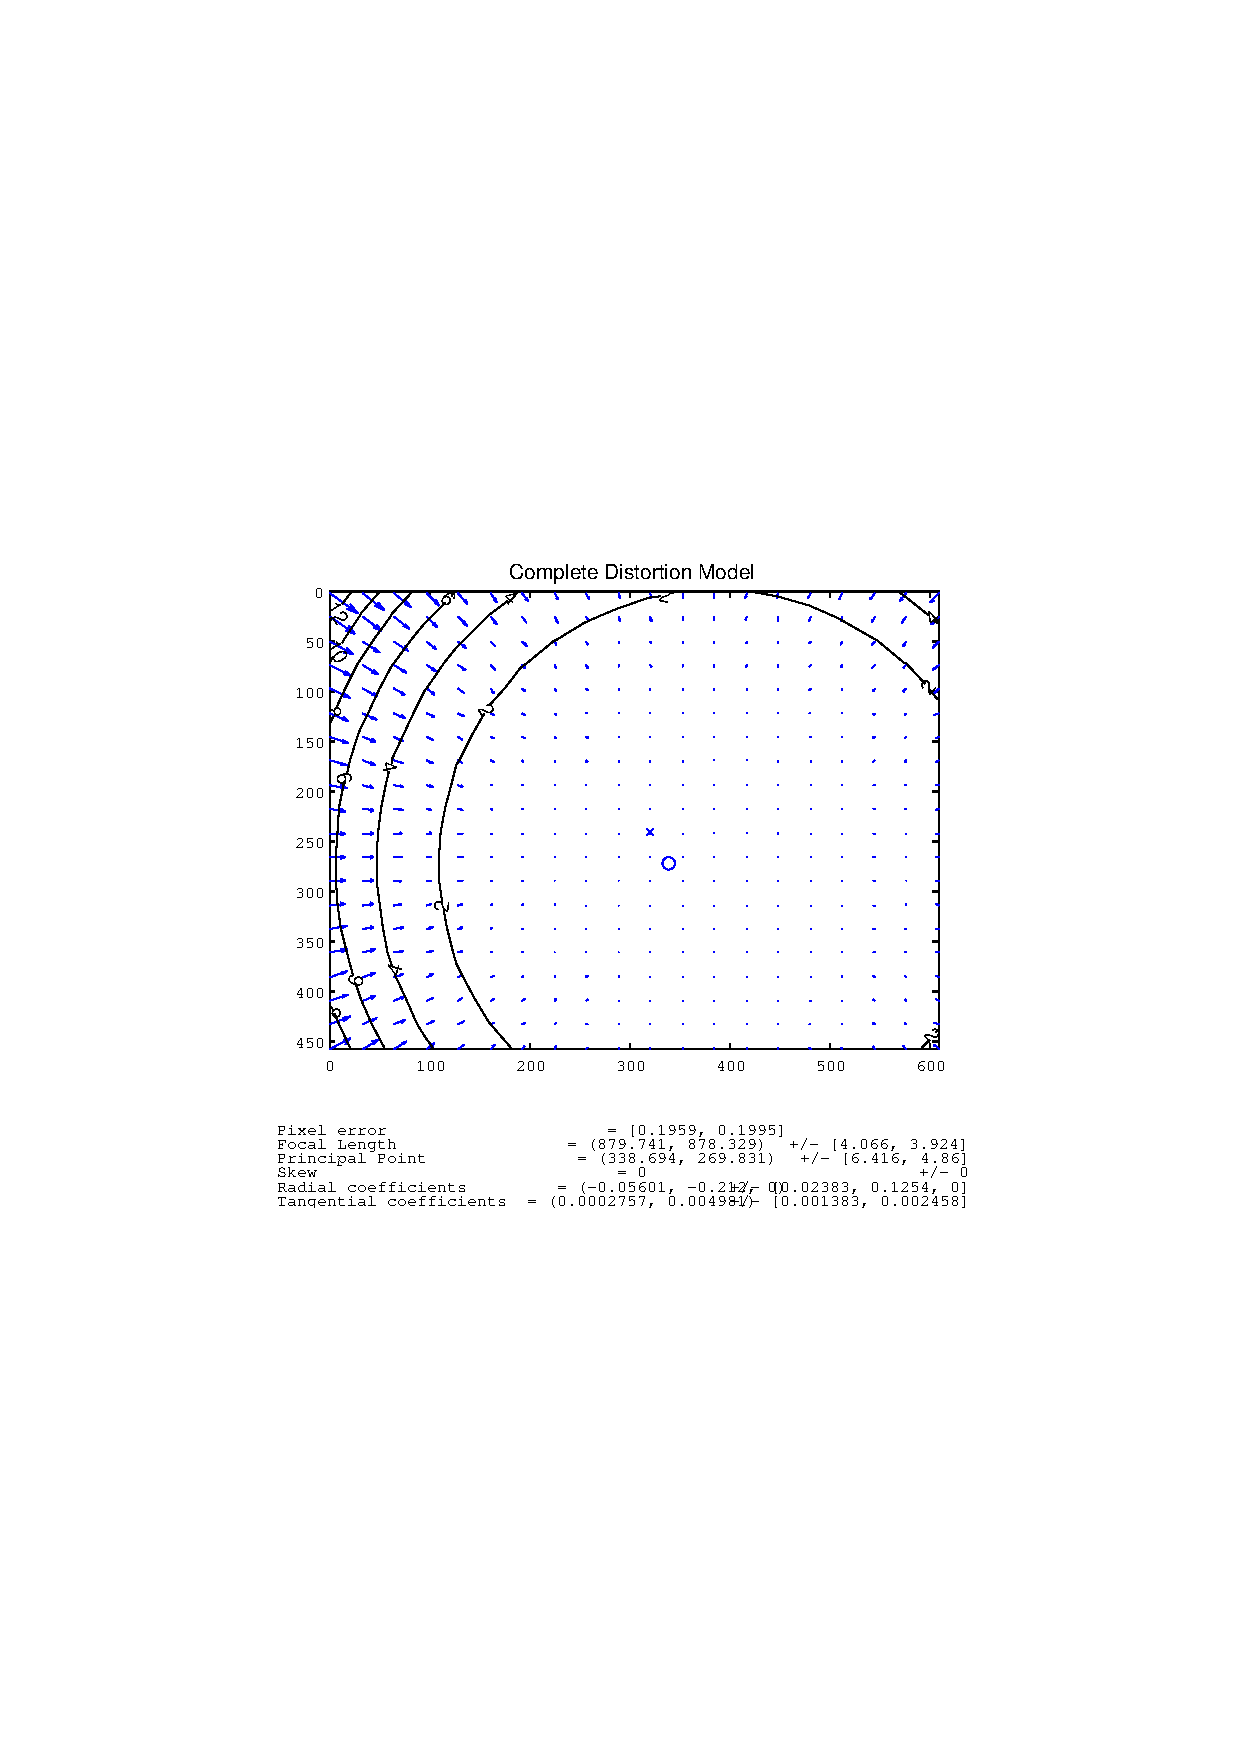
\includegraphics[width=0.47\textwidth]{pics/right_comp_dist}
    \caption{The left and right camera distortion due to lens nonlinearities}
    \label{chap3:fig-comp-lensdist}
\end{figure}
The Figure clearly shows that the principal axis are offset from the center of the images,
and that it is opposite for the left and right images. This means that the view field of
the two cameras will be quite different, and result in a reduced field-of-view for the
total stereo rig.

The intrinsic parameters for the cameras are summarized in Table
\ref{chap3:tab-intrinsic-stereo}. The values are all in pixel coordinates. The real focal
distances can be calculated by knowing the pixel-to-length ratio.
\begin{table}[htbp]
  \centering
    \begin{tabular}{|c|c|c|} 
        \hline
                & Left Camera       & Right Camera \\
        \hline
        $f_x$   & $877.11\pm 2.94$  & $880.28\pm 3.08$  \\
        $f_y$   & $876.49\pm 2.88$  & $879.20\pm 2.96$  \\
        \hline
        $c_x$   & $350.00\pm 6.32$  & $338.54\pm 6.21$ \\
        $c_y$   & $214.30\pm 4.65$ & $267.59\pm 4.35$  \\
        \hline
    \end{tabular}
    \caption{Intrinsic parameters of the stereo rig in pixel related units including
    uncertainties}
    \label{chap3:tab-intrinsic-stereo}
\end{table}
The focus distances in the x and y-direction are slightly different in both cameras. This
suggests that the pixels of two cameras are not exactly square. The principal axis in both
cameras are also in very different places. This is problematic because a stereo rig should
be horizontally aligned to give the best results. Because for the off-center principal
axis the field-of-view of the stereo rig will be quite reduced.

The extrinsic parameters of the stereo rig are estimated based on the displacement of the
checkerboard corners in the different views. The estimated extrinsic parameters are as
follows. The values are given in millimeters. 
\begin{equation}
    T = \left[ \begin{matrix}
                -60.45 \pm 0.18\\
                -0.38 \pm 0.15\\
                -0.02 \pm  1.13 \end{matrix} \right] \quad 
    r = \left[ \begin{matrix}
                0.01 \pm 0.01\\
                -0.01 \pm 0.01 \\
                0.00 \pm 0.00  \end{matrix} \right]
\end{equation}
The baseline given by the manufacturer is 6 cm which correspond very good the estimated
values.
\begin{figure}[hbtp]
    \centering
    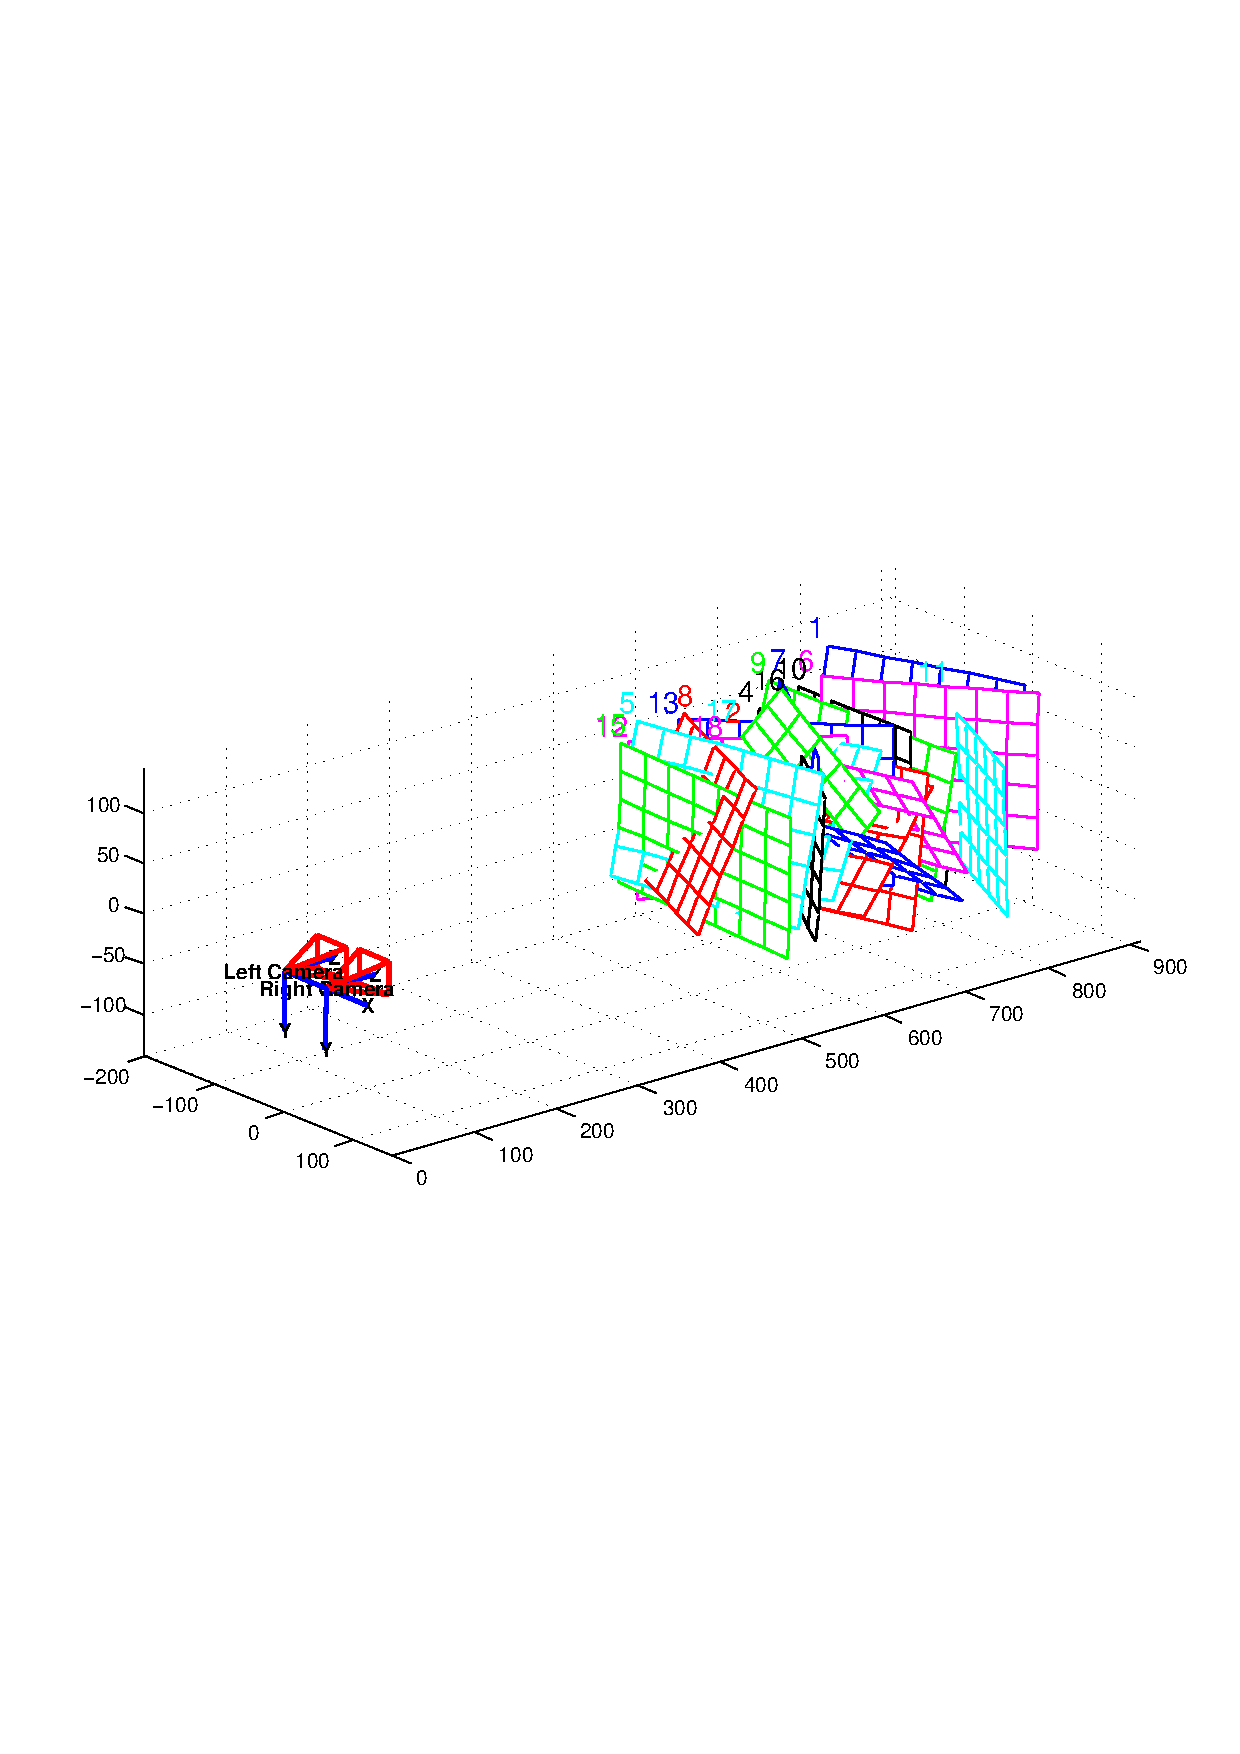
\includegraphics[width=0.7\textwidth]{pics/stereo-extrinsic}
    \caption{The extrinsic calibration of the stereo rig, showing the calculated position
    of the checkerboard sequence}
    \label{chap3:fig-stereo-extrinsic}
\end{figure}


This distortion can be removed and are called rectifying the image. This makes common
features in the two images aligned horizontally. This makes it much easier for the matching
algorithm because it only need to match vertically.


\subsection{Depth resolution}
The depth resolution which can be expected from the Stereo cam are,
\begin{equation}
    \Delta Z = \frac{Z^2}{f T}\Delta d
\end{equation}
where $\Delta d$ is the smallest increment in disparity, $f$ is the focal distance, and
$T$ is the baseline. This is determined in the implementation in this case the OpenCV
library. This is useful when calibrating the stereo rig, and when testing the program,
because it tells what kind of ranges one can expect from the rig.


\subsection{Noise- and Error Sources}
The major source of errors connected with stereo cameras are bad feature matches. This
will cause bogus distances. This is heavily correlated with the amount of noise captured
by the imaging sensors and other disturbances.

As said above, the left and right cameras does not synchronize, and because of the
capturing process is sequential the images are not captured at the same time, this might
give raise to erroneous range measurements. 




\section{Time-of-Flight Camera MESA SwissRanger-3000}
The 3D sensor chosen for the project is the MESA SwissRanger-3000 Time-of-Flight Camera.
This is based on amplitude modulation of near-infrared light (850 nm), which is emitted from an
array of 55 LEDs and captured at a spherical PMD chip. The spatial resolution of the camera
are $176\times144$ with a field-of-view of $47.5^\circ \times 39.6^\circ$. 
\begin{figure}[htbp]
    \centering
    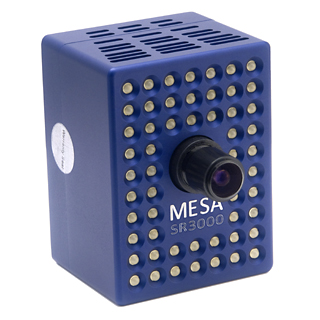
\includegraphics[width=0.4\textwidth]{pics/sr3000}
    \caption{The SwissRanger-3000 Time-of-Flight Camera. \url{http://www.mesa-imaging.ch}}
    \label{chap3:fig-sr3000}
\end{figure}
The amplitude modulation frequency are set to 20 MHz which gives a non-ambiguity range of
7.5 meters. If the modulation frequency is lowered the maximum measured distance might be
larger, but this distance is good for the application of the project. 

Since the camera needs lots of cooling because of the LEDs and electronics the camera are
mounted on a stem of aluminium, to secure the airflow through the camera. 

The camera outputs standard Cartesian coordinates or spherical coordinates and the
intensity, which is comparable to a standard gray scale camera. Figure 
\ref{chap3:fig-tof-amppicture} shows a typical amplitude plot of the inside of a pipe. The
blue areas are closer, and red areas are farther away. 
\begin{figure}[htbp]
    \centering
    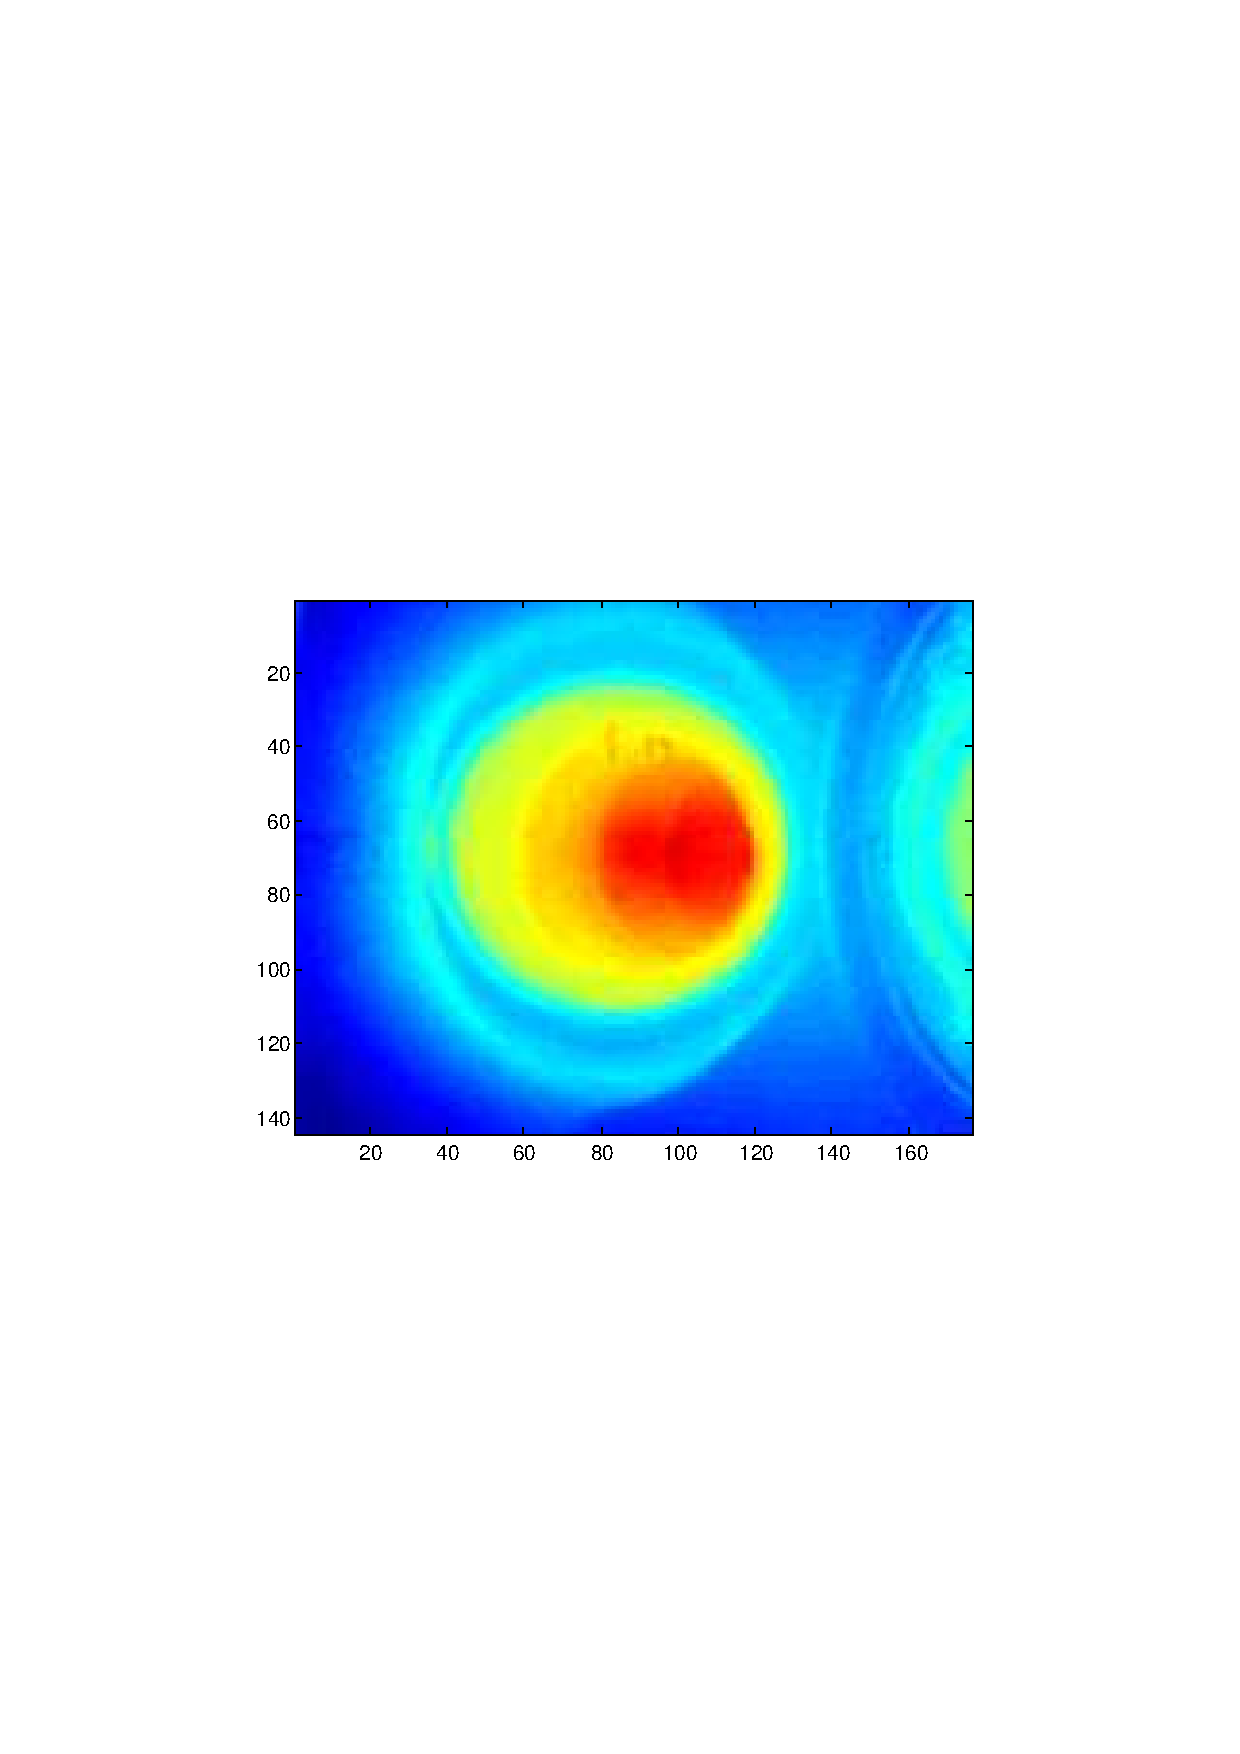
\includegraphics[width=0.8\textwidth]{pics/tof-amppicture}
    \caption{Typical amplitude image of the SR-3000 ToF-camera}
    \label{chap3:fig-tof-amppicture}
\end{figure}


\subsection{Intrinsic Parameter Calibration}
The intrinsic parameters are determined the same way as for the individual cameras in the
stereo rig. This is to determine the lens distortions and principal axis, see Table
\ref{chap3:tab-intrinsic-sr3000}.
\begin{table}[htbp]
  \centering
    \begin{tabular}{|c|c|c|} 
        \hline
                & SR-3000       & Given by Manufacturer \\
        \hline
        $f_x$   & $212.52 \pm 14.91 $  & $200$  \\
        $f_y$   & $213.94 \pm 14.96 $  & $200$  \\
        \hline
        $c_x$   & $88.63 \pm 5.00$  & $88$ \\
        $c_y$   & $ 62.96 \pm 5.67 $ & $72$  \\
        \hline
    \end{tabular}
    \caption{Intrinsic parameters of the ToF-camera in pixel related units including
    uncertainties}
    \label{chap3:tab-intrinsic-sr3000}
\end{table}
The focal distances given from the manufacturer are calculated using the pixel size of
$40 \times 40 \mu m^2$ and 8 mm focal distance.

The calibration method is the same as for the stereo cameras. The intensity images from
the camera are captured, converted to 8-bit integer values and histogram normalized to
enhance give better contrast. This makes the finding of the checkerboard corners easier in
the calibration process. Since the spatial resolution of the camera are small, noise and
inaccurate sampling make the corner selection problematic. This shows itself on the large
uncertainties int in the focal distances. 

\begin{figure}[htbp]
    \centering
    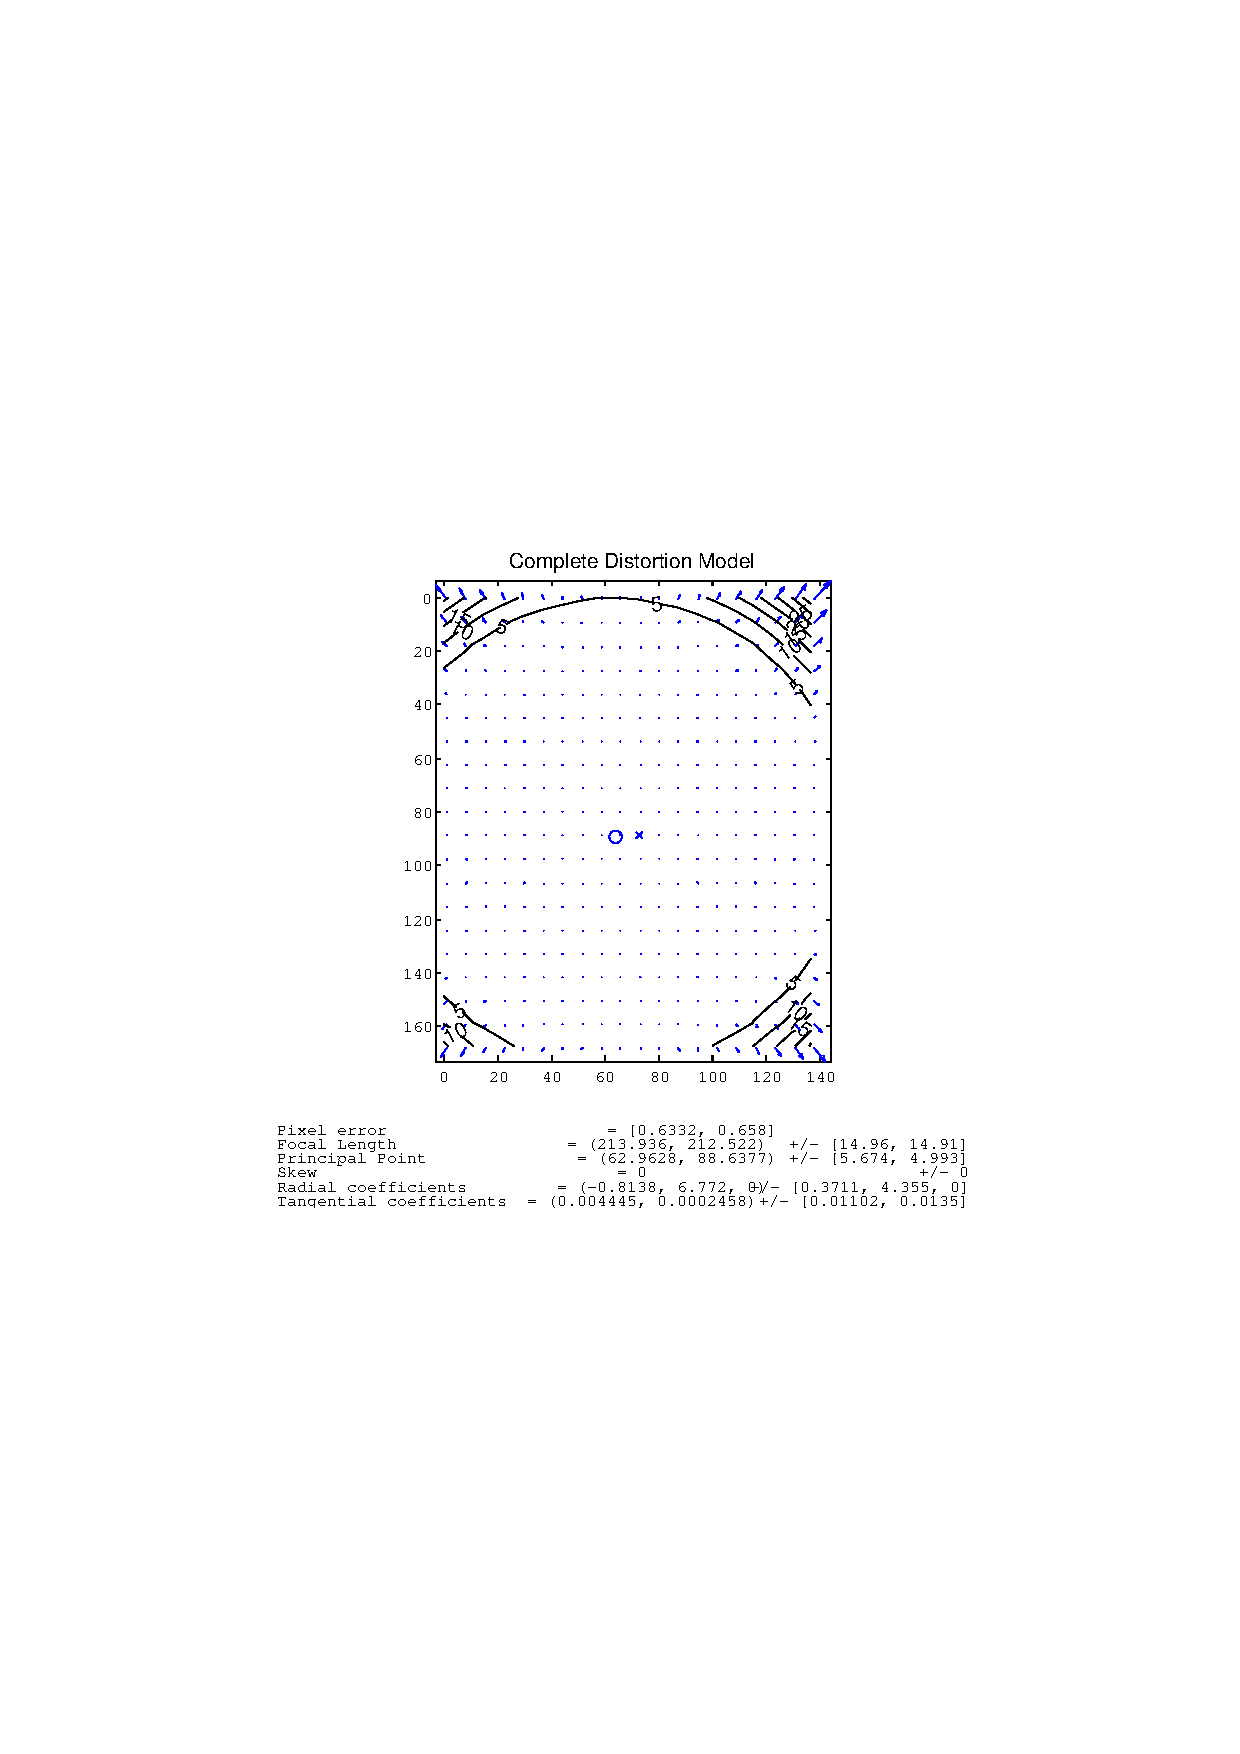
\includegraphics[width=0.7\textwidth]{pics/sr3000_comp_dist}
    \caption{The lens distortion for SwissRanger 3000}
    \label{chap3:fig-sr3000-comp-lensdist}
\end{figure}
From the Figure \ref{chap3:fig-sr3000-comp-lensdist} the distortion due to lens are shown.
The principal axis are off center in the y-direction, this might be the case, but can also
be inaccuracies caused by the calibration. Except for this off-center principal axis, the
pixel distortion due to the lens is small.


\subsection{Depth Calibration}
\label{chap3:subsec-depht-calib}
Depth calibration of the \emph{SR3000} to remove the systematic errors due to
imperfections in the creation of the sinusoidal correlation signal was not done, 
because the inaccuracies in depth
were thought to be of less importance with regard to the project. Using the depth
calibration proposed in \cite{sr3000} or \cite{tof-calibration} would probably give a
smoother point cloud, and ease the work for the higher level control system. But these
systems must be robust, and an uncalibrated sensor will help test this. 



\subsection{Noise- and Error Sources}
As stated in Section \ref{chap2:subsec-tof} the complete picture of the distances are
captured fist when 4 successive exposures are complete. This means that fast moving
objects will cause distance errors because the object might have moved between the
exposures. Another source of errors are multiple reflections and highly reflective
surfaces which will cause errors because too much light is reflected. The same is the case
with surfaces which absorbs most of the light. This surfaces will appear farther away than
they really are. 


\section{Sensor Configurations}
\label{chap3:sec-sensorconfig}
\begin{figure}[htbp]
    \centering
    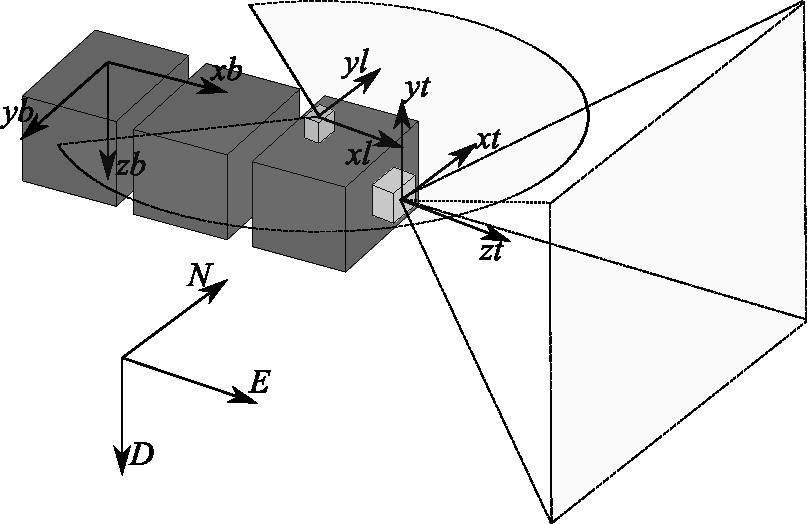
\includegraphics[width=0.7\textwidth]{pics/sensor-config}
    \caption{The different reference frames}
    \label{chap3:fig-sensor-frames}
\end{figure}
The different reference frames are shown in Figure \ref{chap3:fig-sensor-frames}, together
with the field-of-view and domains of the senors. These are the
\emph{North-East-Down} frame, \emph{body} frame, and the two sensor frames with
corresponding field of view. All of the systems are defined as right-hand-systems. 

For the system it is important to known the location of the different sensors, relative to
the center of gravity of the platform, where usually the center of the body frame are
defined. 





%\chapter{Sensor Fusion}



\section{Kalman Filter}



\section{State-of-the-Art sensor fusion}





%file included in thesis.tex


\chapter{Data Representation}


\section{Map-building From the Sensor Data}


\section{Sensor Data Processing}


\subsection{Edge-detection Algorithms}


\subsection{Other Feature Extraction}







%file included in thesis.tex

\chapter{Implementation}
In this chapter implementation specific issues are treated. Figure
\ref{chap6:fig-implementation} shows the three-layer implementation of the project.
\begin{figure}[htbp]
    \centering
    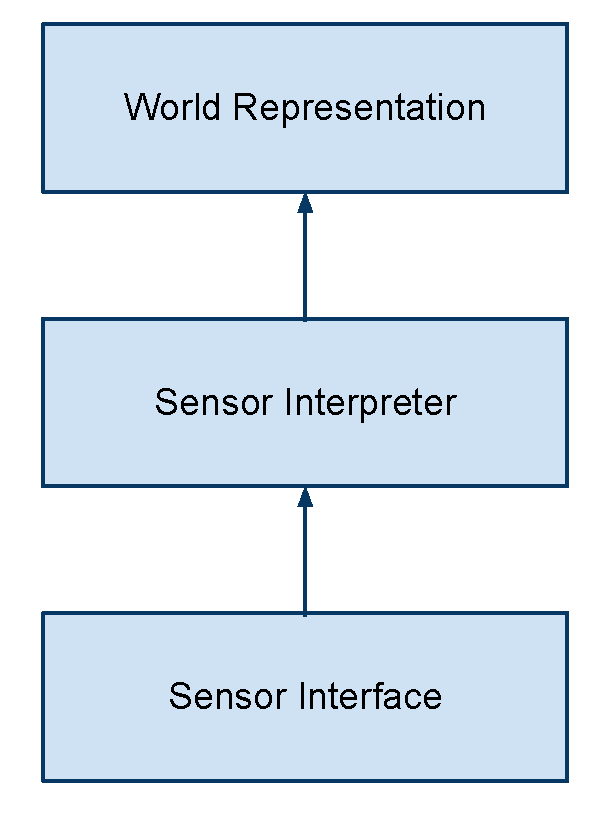
\includegraphics[width=0.4\textwidth]{pics/implementation}
    \caption{Three-layer implementation}
    \label{chap6:fig-implementation}
\end{figure}
The \emph{low-level} layer reads and converts the raw sensor data into common data which can be
interpreted by the \emph{middle} layer. This layer handles all the ''washing`` of the
sensor data, and applies the reasoning and tries to recognize the environment. The third
and last layer is the \emph{world} layer which handles the global data, where the robot is
and where it should move next. 

The project is implemented in both \emph{C/C++} and Matlab. The sensor layer are
implemented in \emph{C/C++} while the other layers are implemented in Object-Oriented
Matlab. 

\section{Low-level Interfaces}
The low-level interfaces from the sensors are implemented in \emph{C/C++} and uses the
supplied sensor APIs. The SwissRanger 3000 API were used directly in Matlab. The Hokuyo
API was a little more tricky to use. A Matlab interface function were implemented to get
the sensor data directly into Matlab.

\subsection{Stereo Camera Implementation}
For the stereo camera, a program was written using the \emph{OpenCV} library. A open
source computer vision library, initially developed by Intel. This library have many
excellent and optimized functions for grabbing images, camera calibration, image rectification
and stereo matching. This produced a disparity map, which again where reprojected into 3D
by the \emph{cvReprojectTo3D()}-function. This coordinate images where saved to disk and
read into Matlab for further processing. 

\begin{algorithm}
\caption{The Stereo Capture Procedure}
\label{chap6:alg-stereomatch}
    \begin{algorithmic}
    \STATE \textbf{begin}
    \STATE Connect to Cameras
    \FOR{no of images $<$ 20}
        \STATE Capture images of Checkerboard and find corners
    \ENDFOR
    \STATE Calculate the distortion parameters using Healy's Method.
    \WHILE{Not Quitting}
        \STATE Capture images
        \STATE Rectify Images
        \STATE Stereo matching using Block Matching 
        \STATE Reproject disparity map to 3DImage
        \STATE Dump 3D Coordinates to Disk
    \ENDWHILE
    \STATE \textbf{end}
    \end{algorithmic}
\end{algorithm}
This program calibrates the cameras, rectifies the images, finds stereo correspondences
and reprojects them to 3D coordinates.


\section{Mid-level Implantations}
The middle layers goal is to process and interpret the sensor data to best ability. This
layer is in charge of doing the reasoning, and draw out important information form the
sensor data. The main task is to find lines in the 2D sensor data, and cylinder shapes in
the 3D data. 

This functionality are implemented in a Matlab class called the \emph{SensorInterpreter}.


\subsection{Analysis of 3D Sensor Data}
The 3D data are first filtered with regard to corresponding the intensity image. Pixels
with intensities larger or lower than a threshold value will be filtered away and set to
zero. 

After this the coordinates are sorted on ascending depth value, and all trivial points,
i.e. zero points are taken out of the coordinate list. The new list with coordinates
including only interesting points will be divided into 10 equally spaced bins in the depth
direction. Each of this bins are sent to the surface fit algorithm which is a
\emph{Least-Squares Guass-Newton steepest decent}-algorithm. 

\subsubsection{Surface Fit Algorithm}
The algorithm which is used are the \emph{EUROMETROS}\cite{eurometros} Matlab library developed by
\emph{National Physics Laboratory(NPL)} in the United Kingdom. The algorithm provides the
estimated radii, and directions of the data sets. Also the distance of the data set to the
estimated cylinders are output, which is a measurement on how good the cylinder fit is. 


\section{High-level Implementations}

\subsection{World Representation}
The world representation are implemented as objects in Matlab. Each node in the world
representation described in Chapter \ref{chap5} are implemented as a class in Matlab. 
\begin{figure}[htbp]
    \centering
    %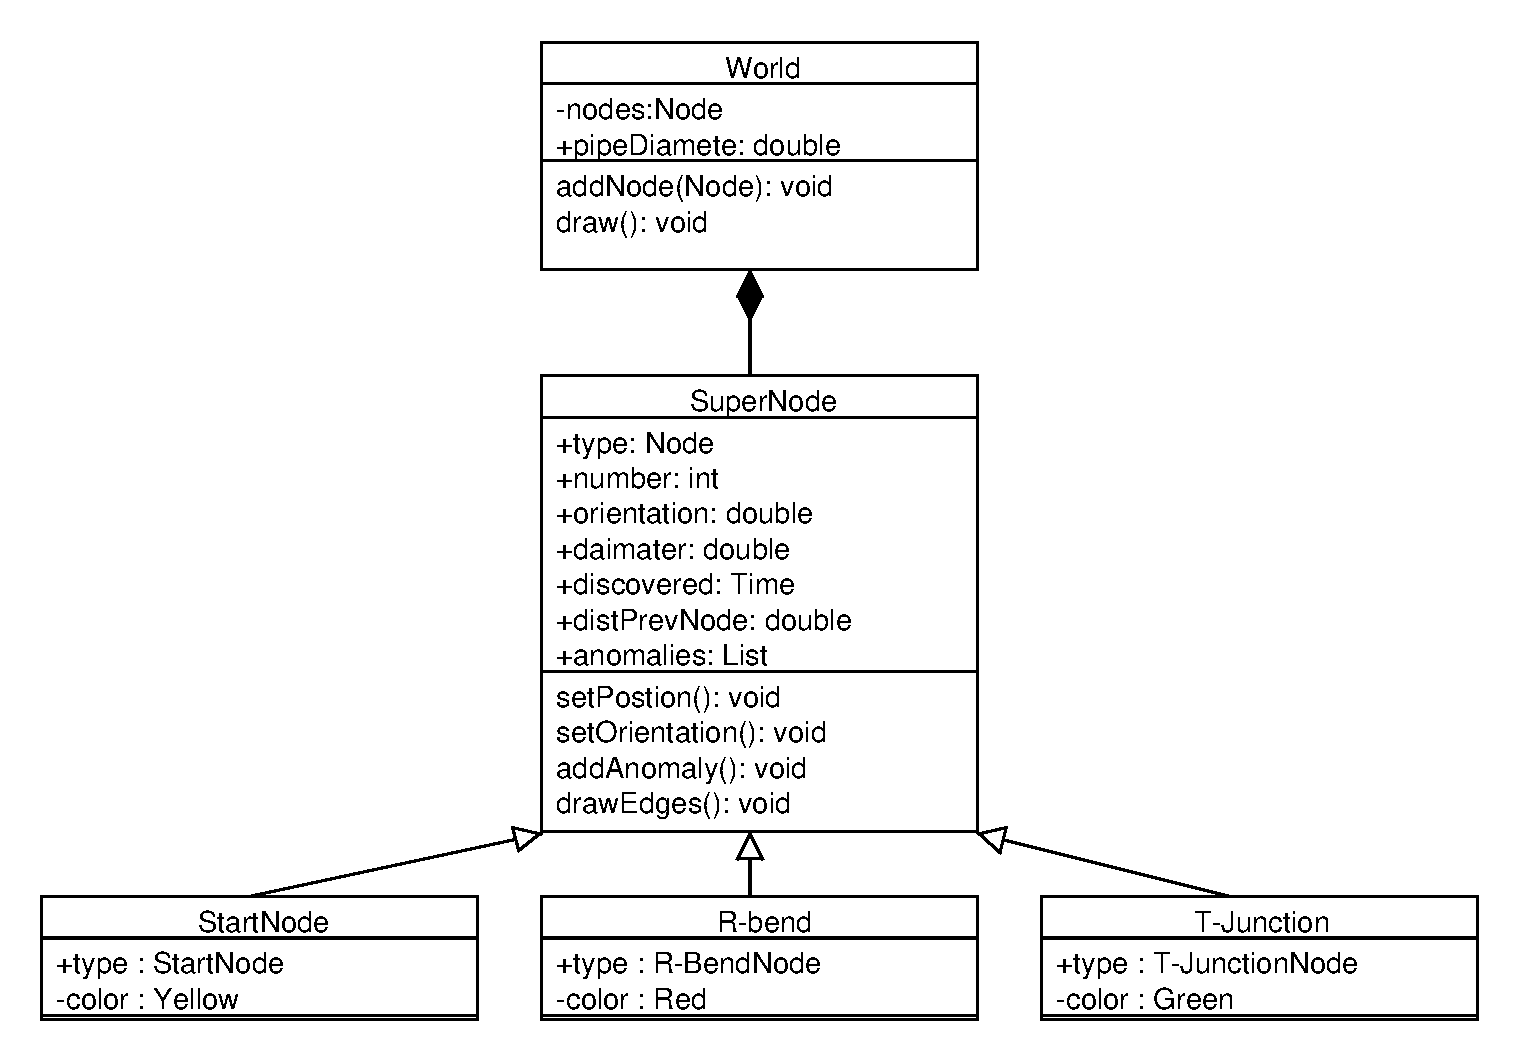
\includegraphics[width=0.6\textwidth]{pics/world-uml}
    \caption{UML of the world representation}
    \label{chap6:fig-world-uml}
\end{figure}

As seen from Figure \ref{chap6:fig-world-uml} the implementation are based on a
\emph{world} class which contains the á priori map of the world and the node network
together with some useful parameters. The nodes of the representation are also different
classes which inherits from a super node. 


\section{Summary of Parameters}
Here a summary of the different parameters that the user is required to set, and guess, is
given. 
\begin{table}[htbp]
    \centering
    \begin{tabular}{|r|l|}
        \hline
        $LowIntensity$ &  Threshold value for filtering low intensity pixels   \\
        $HighIntensity$ & Threshold value for filtering high intensity pixels  \\
        Interval      &  The interval for which the point cloud should be divided \\
        $m$             &  value which defines $m r_i$ as errenous             \\
        \hline
        $hits_y$    &  The bin sizes of the histogram in the y direction       \\
        $hist_x$    &  The bin sized of the histogram in the x direction       \\
        $NoPointsY$ &  The number of points in a bin to define a line          \\
        $NoPointsX$ &  The number of points in a bin to define a line         \\
        $P_1$       &  The distance of the measurement plane of the URG in meters\\
        $ParallelThreshold$ &  Upper value that defines if two lines are parallel \\
        \hline
        $NoChessBoardImages$ & images of the checkerboard required for stereo camera calibration         \\
        \hline
    \end{tabular}
    \caption{Summary of the user parameters}
    \label{chap6:tab-user-parameters}
\end{table}

\section{What is not Implemented}
There are a number of things that are not implemented because of time issues. Probably the
most important thing is the segmentation of the sensor data. This is crucial for the
least-squares method to work properly. 

Another thing that is not implemented is the module that recognizes and matches pipe
profiles. The idea of this is that it will from the sensor interpreter recognize the pipe
profile, which is matched to some internal database of profiles.

Also, the matching algorithm for finding the global position from the passed-through nodes
have also been skipped for time issues. All, of this modules are easy to insert in the
present implementation, because of the modular architecture. 





\chapter{Testing}
Testing is an important aspect of the work carried out in this thesis. In this chapter the
test setup are described. How the tests are carried out, some of the results and some
imidiate results.


\section{Test Environment}
The test environment are two connected pipe segments. A Y-junction and an L-bend. This
pipe segments are connected, according to Figure \ref{chap7:fig-environment}.

\begin{figure}[htbp]
    \centering
    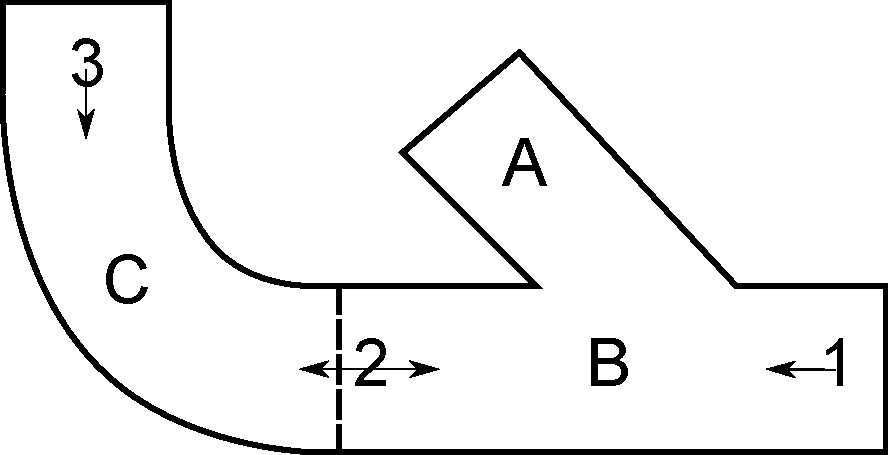
\includegraphics[width=0.7\textwidth]{pics/test-environment}
    \caption{The test environment}
    \label{chap7:fig-environment}
\end{figure}

There are six points of interest in this environment. 
The numbers 1-3 are the places where the sensors will be put and record snapshots of the pipe. 
The letters A-C are places where irregularities and anomalies in the pipes are placed. 


\section{Test Cases}
To test the performance and robustness of the developed algorithms three cases are used,
ideal situation, situation with obstacles with regular surface, and obstacles where the
surface are irregular. This cases are carried out for all the 3 different places described
in the previous section.

The tests are snapshots of the pipe at the given locations. This will test the abilities
of the system to recognize the environment and do the right decision. 


\subsection{Control/Ideal Case}
Here the sensors are placed at the different locations and the output are recorded. This
is for reference and what the data will look like in the ideal case. This should
considered perfect readings and all further readings will be measured up to this.


\subsection{Irregular surfaced anomalies}
The algorithm implemented relies greatly on regularity in the environment. The structure
of the surroundings are known to great extent and all irregularities and differences from
this are considered strange and are marked as anomalies. This case should test if this
works.

The tests are carried out with a curled-up paper which is placed at the three different
locations, marked in Figure \ref{chap7:fig-environment}. 
\begin{figure}[htbp]
    \centering
    \includegraphics[width=0.6\textwidth]{pics/curled-paper}
    \caption{The curled-up paper placed at point A in the pipe}
    \label{chap7:fig-culed-up-paper-at-A}
\end{figure}



\subsection{Regular surfaced anomalies}
As mentioned above the algorithm relies on regularity in the environment to detect
anomalies. This test will try to test the ability of the system to detect regular surfaced
objects which might look as they are a part of the environment. 

A stack of matchboxes are placed at the locations described and the data are recorded.
Figure \ref{chap7:fig-matchboxes-at-C} shows a picture of the stack of matchboxes placed
at Point C.
\begin{figure}[htbp]
    \centering
    \includegraphics[width=0.6\textwidth]{pics/matchboxesC}
    \caption{Stack of matchboxes placed at Point C}
    \label{chap7:fig-matchboxes-at-C}
\end{figure}



\section{Test Results}







\chapter{Discussion}
\label{chap8}
This chapter will evaluate how the implemented algorithms work, the shortcomings and
possible solutions to problems. 

\section{How did it perform?}
How the system preformed are outlined in this section. Starting off with the
\emph{SwissRanger 3000} Time-of-Flight camera.

\subsection{MESA SwissRanger 3000}
To start off, the output from the camera were applied directly into matlab. Default
integration time were used, and the intensity- and range images where captured as is from
the camera electronics.

The default readout from the ToF camera were not that affected by the difficulties
described in Chapter \ref{chap2}, but the individual range values where dominated by normal
distributed measurement errors. This where removed by averaging the images over a number
of successive images. This reduced the response time of the sensor and therefor the
refreshment time, but this will most probably not be a case in this application, since the
velocities included are not of the greatest magnitudes. 

Figure \ref{chap8:fig-typical-tof-image} shows a typical range image, and the
corresponding intensity image. 
\begin{figure}[htbp]
    \centering
    %\includegraphics[width=0.8\textwidth]{pics/tof-imagery}
    \caption{Typical range image of the pipe}
    \label{chap8:fig-typical-tof-image}
\end{figure}

When objects came too close to the sensor, it looked like the sensor went berserk. This
was because the intensity values became so large, and they dominated the picture
completely. The solution to this were to filter the range image based on the intensity
value of that pixel. An example of this can be seen in Figure
\ref{chap8:fig-tof-imagery-intensity-filtered}
\begin{figure}[htbp]
    \centering
    %\includegraphics[width=0.45\textwidth]{pics/tof-intensity-unfilterd}
    %\includegraphics[width=0.45\textwdith]{pics/tof-intensity-filtered}
    \caption{The unfiltered and filtered point clouds}
    \label{chap8:fig-tof-imagery-intensity-filtered}
\end{figure}



\subsection{Minoru 3D webcamera}
The stereo camera rig which is used in the project is a cheap mass produced stereo
webcamera. As seen from the calibration in Chapter \ref{chap3} the two different cameras have substantial
distortion, both tangential due to misaligned CCD chip, and radial due to cheap optics.
Unfortunately, the CCD chips are horizontally aligned right, while in the vertical
direction they are aligned in a divergent way. This will limit the field-of-view of the
camera. The principal axes of the two cameras are unaligned horizontally, which will
further limit the field-of-view. See figures \ref{chap2:fig-tang-dist},
\ref{chap3:fig-comp-lensdist} and \ref{chap8:fig-rad-dist}.
\begin{figure}[htbp]
    \centering
    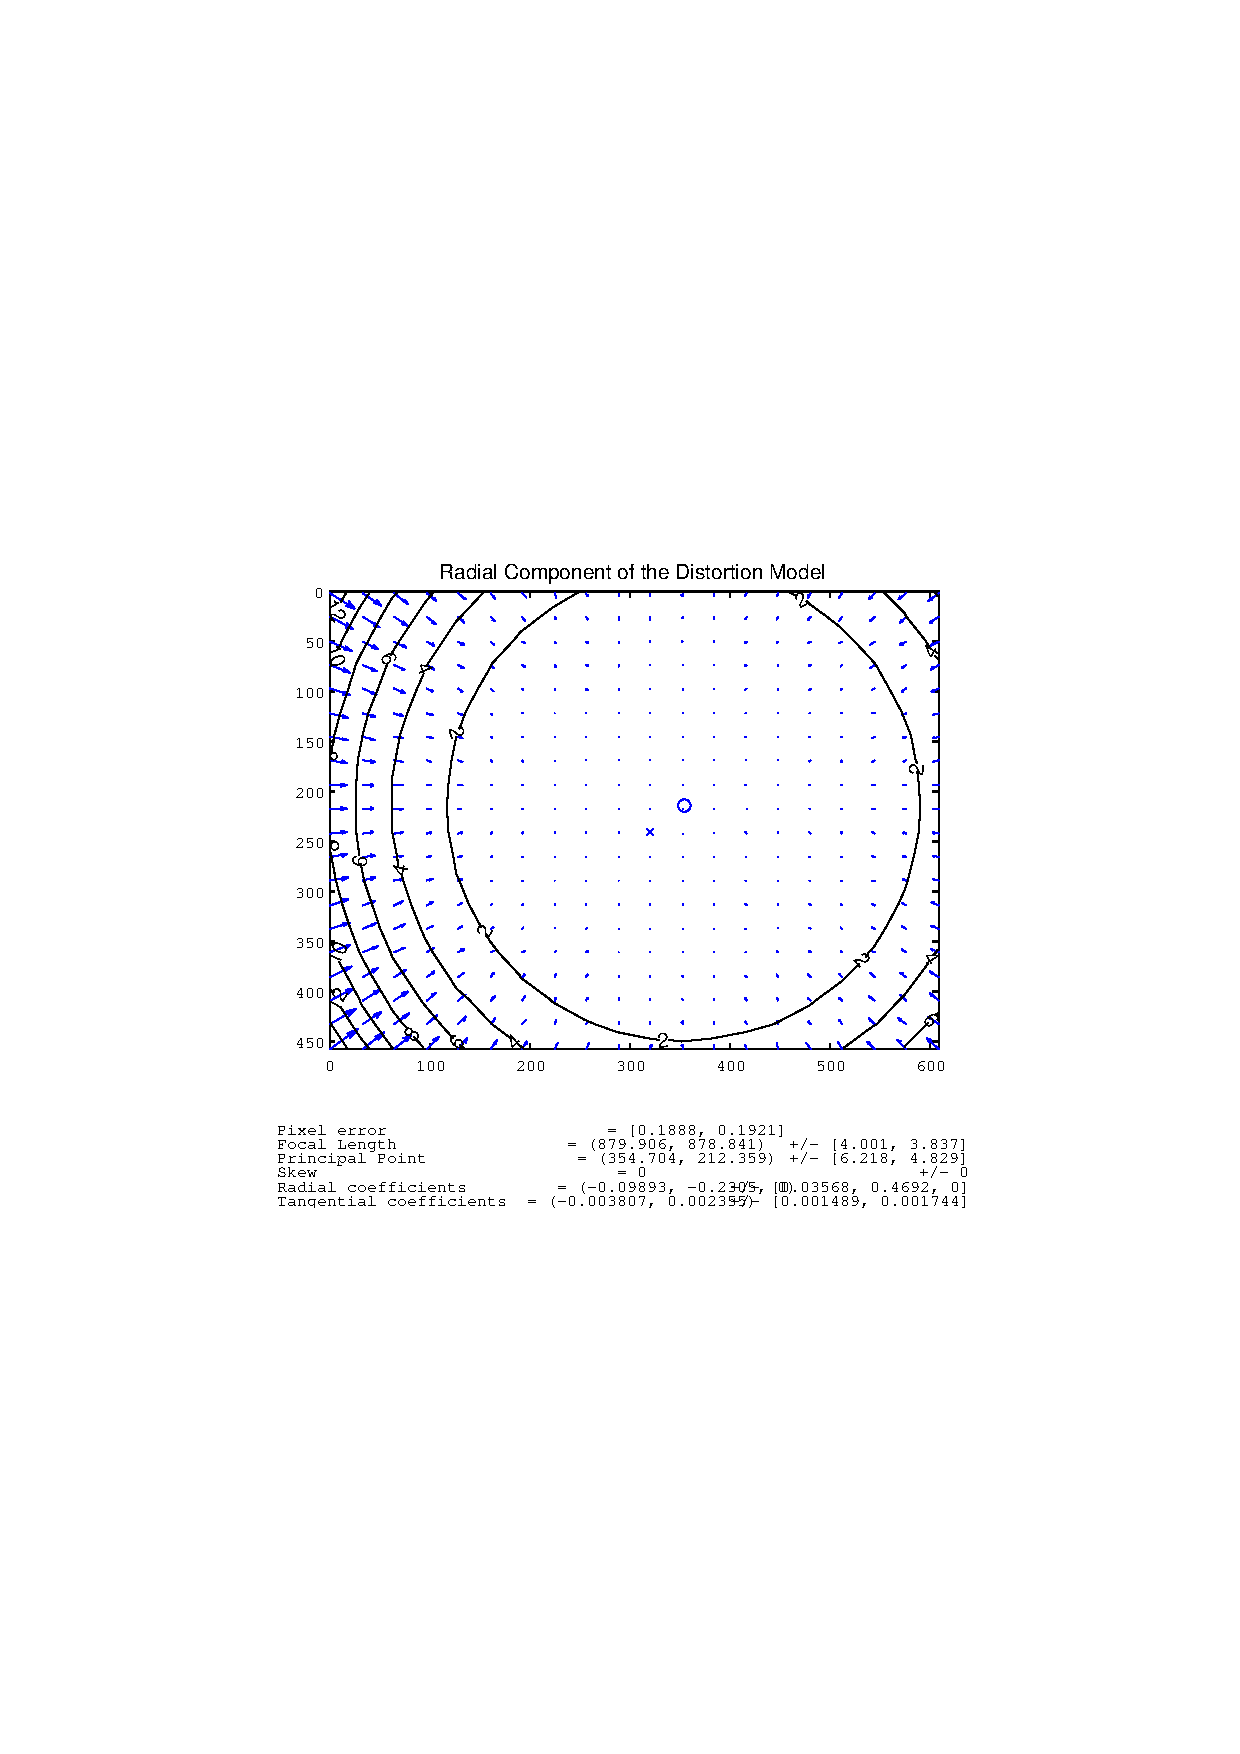
\includegraphics[width=0.45\textwidth]{pics/left_rad_dist}
    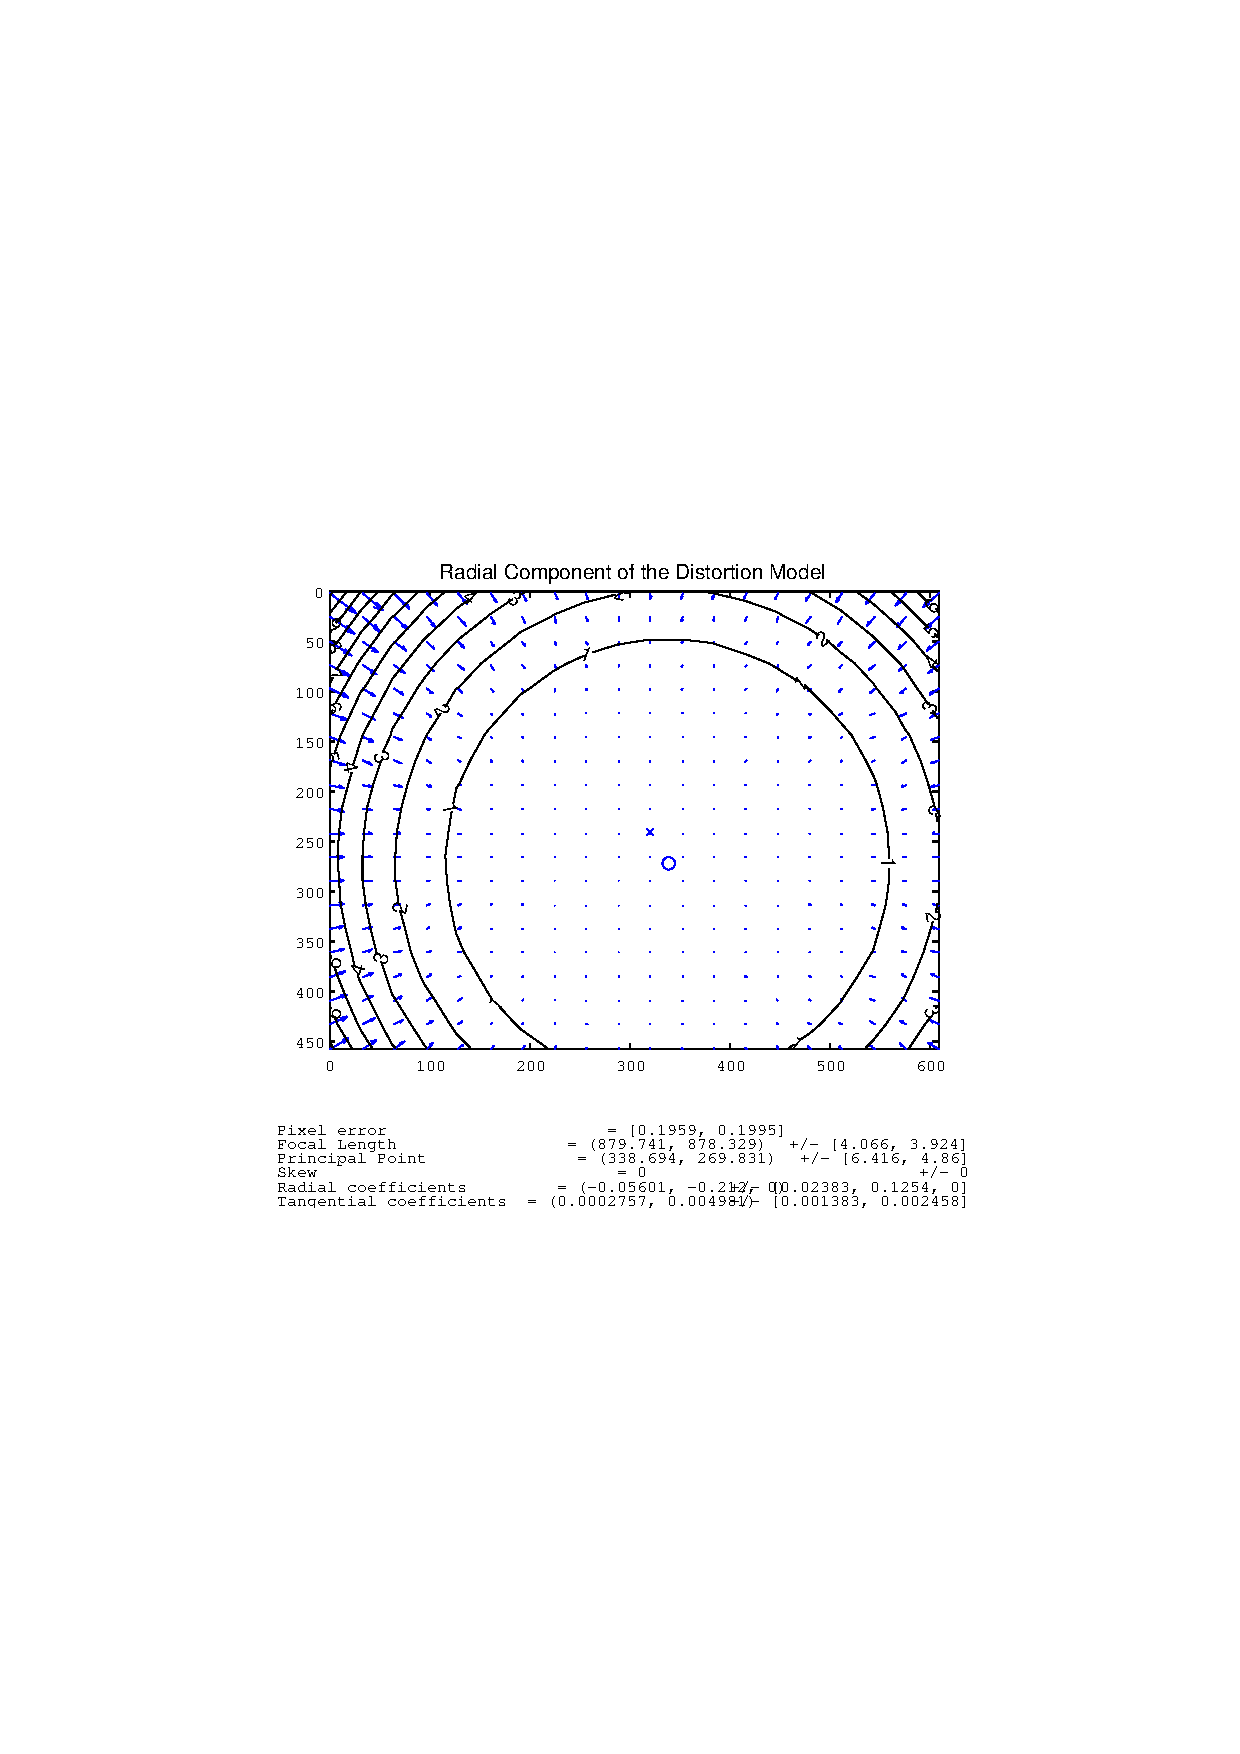
\includegraphics[width=0.45\textwidth]{pics/right_rad_dist}
    \caption{The radial distortions of the left and right camera of the stereo rig}
    \label{chap8:fig-rad-dist}
\end{figure}
The field-of-view of the stereo rig is the incision of the two images. 

Another limit of the cameras, besides the field-of-view is the light sensitivity and
the amount of noise on the captured images. The amount of noise in the captured pictures
are dependant on the portion of ambient light in the scene. In the tests no extra
light source where used, only ambient and sunlight from the surroundings. This was because
the pipe bends where turned towards the window which gave much sunlight. If a artificial
light source were included in the tests, some of the features would be sharper and the
matching would have produced better results. 

The inside of the test pipe were mostly featureless. The implemented algorithms did not
detect enough features in both cameras to calculate a dense stereo image of in most of the
cases. 

Even when there were obstacles, both irregular and regular objects, the algorithm did not
detect enough features, and where not able to match these features. This might be because
that there were not enough light in the scene, and the surfaces of the irregular object
where not sharp enough for the algorithm to detect. 

To test if the algorithm did provide dense stereo images, the stereo rig were directed at
a typical lab environment, with enough structure to make good stereo matches for the
implementation. See figures \ref{chap8:fig-structured-test-rectified} and
\ref{chap8:fig-structured-test-depth}
\begin{figure}[htbp]
    \centering
    %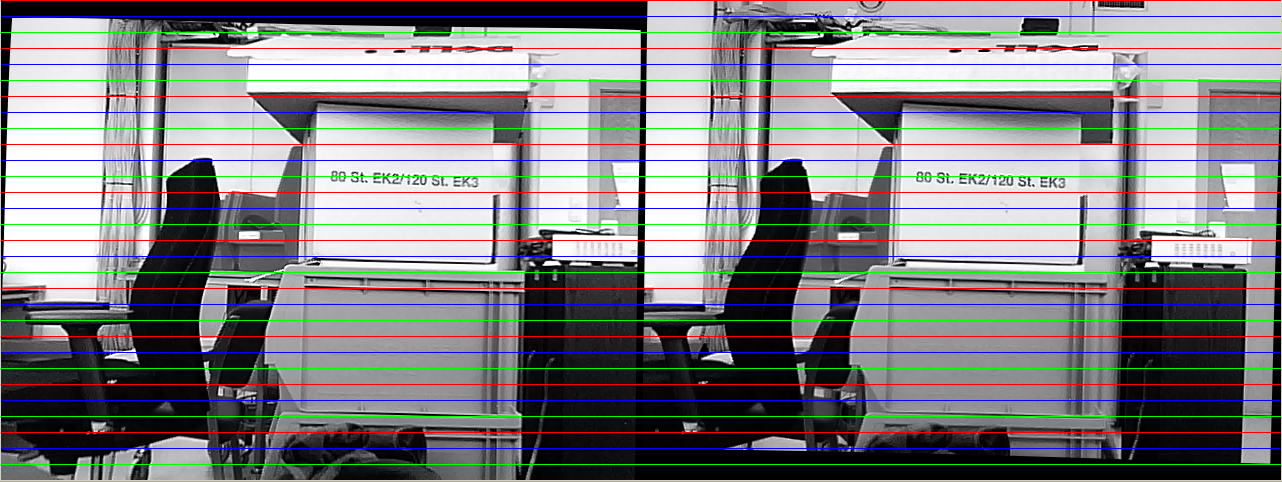
\includegraphics[width=0.8\textwidth]{pics/structure-test-rectified}
    \caption{Rectified left and right images of the structured lab environment}
    \label{chap8:fig-structured-test-rectified}
\end{figure}
\begin{figure}[htbp]
    \centering
    %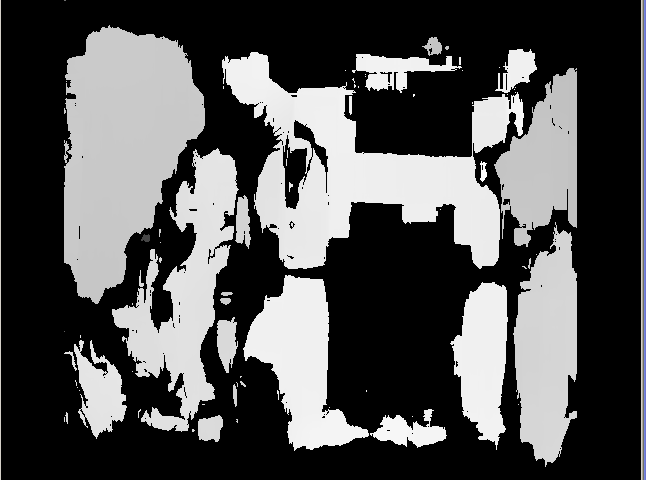
\includegraphics[width=0.45\textwidth]{pics/structure-test-depth}
    %\includegraphics[width=0.45\textwidth]{pics/structured-test-3d}
    \caption{Depth image and projected point cloud of the structured lab environment test}
    \label{chap8:fig-structured-test-depth}
\end{figure}
This clearly shows that the algorithm works adequately for good lit, structured
environments. The depth image is represented in pixel related units. Since the exact size
of the pixels on the CCD chip were difficult to come by, the distances are given in
pixels. It can be seen that the range image is much more detailed, this is most probably
because there are sufficient light in the scene and a lot more features which can be
matched.

When regarding speed, the \emph{OpenCV} library are reasonable fast. When running at
$640\times480$ a brute-force implementation of the stereo matching using standard
\emph{OpenCV}-library methods, where able to process 2-3 stereo pairs each second, and
output a dense stereo range image, on a Pentium 4 3.0 GHz Windows XP standard workstation
with 2 Gb of RAM. 



\subsection{Hokuyo URG-04LX Laser Range Finder}
The measurement from the laser range finder that affects the readings in the test were
mostly random gaussian distributed noise. To get rid of this, 5 successive
readings where averaged. Since the update rate of the range finder is 10 Hz, the system
will get readings from the URG twice every second. This will not impact the control system
that much, since the dynamics of the system is not that fast. The implementation, the time
needed to get a full range scan was about 0.1-0.15 seconds. The times seemed a bit random,
and where dependant on the time to locate enough memory to store the scan.. The times
seemed a bit random, and where dependant on the time to locate enough memory to store the
scan.. The times seemed a bit random, and where dependant on the time to locate enough
memory to store the scan.. The times seemed a bit random, and where dependant on the time
to locate enough memory to store the scan. 




\section{Why did it perform this way?}







\chapter{Conclusions}
\label{chap9}
This report have proposed a partial navigation system for a pipe inspection robot using three
types of sensors, namely a Laser Range Finder, a Time-of-Flight camera and a stereo
camera. The system uses a modular three-layer approach, where the lower layer is the
sensor layer. Transforms the sensor information into a common coordinate
representation. The middle layer handles the interpretation of the sensor data, which include cylinder fit-
and line fit algorithms. The third layer handles the world representation, that keeps track of
the current explored areas. Further, pipe profile matching, path planning algorithms and command
algorithms might be implemented in the third layer.

The different sensors have been investigated, their abilities have been
evaluated, and possible difficulties by using the proposed sensors have been evaluated.
The results show that the laser range finder provides reliable results in the plane without much
filtering and treatment of the sensor data. It does however only provide measurements in the
plane, which means that it easily misses obstacles that are close to the ground and does
not cross the measurement plane of the 2D sensor. 

The time-of-flight camera on the other hand,
need more preparation before it can be utilized to create a map of the surroundings,
mostly because it provides more denser information, and this information is more prone to
noise. The intrinsic parameters of the camera were determined, and corresponded well to
the values given by the manufacturer. No calibration for the range data were preformed, 
mostly because it where thought not to impact the system performance significantly. 

The stereo cameras intrinsic parameters and lens distortion coefficients were estimated.
As expected this showed severe distortions and offset of the principal axes which impacted
the field-of-view of the stereo rig. The cameras did not preform that well in the given
environments, mostly due to the quality of the camera, and the lack of synthetic
lighting in the scene. Some enhancement of the images might have given better matching
results, but this were not tested.

A proposed representation scheme of the sensor data were also implemented. This is a
topological representation of the world, which is based on much reasoning and
interpretation of the sensor data. A set of nodes are defined. This can be pipeline
junctions, like a $90^\circ$-bend, or a T-junction and likewise. It can also be any other
feature that is not like the usual featureless straight pipeline. As said previously, this relies
greatly on the interpretation of the sensors, which prove difficult with the proposed
algorithms. Although no matching algorithms from the sensor data to the world
representation is proposed, the topological approach for the world representation were
chosen because of the simple and demanding less memory than other mapping approaches, for
example the occupancy grid approach, which is quite spacious when keeping track of a three
dimensional world. 

The implemented sensor interpretation algorithms did not work according to the expected
results. The algorithms are least-squares based algorithms, and this does not work well when
no selection of the dataset was preformed. The topic of segmenting a data set into
different regions are a difficult but crucial topic when the interpreting sensor data from
complex scenes. Unfortunately, time did not allow for developing a good solution to this
problem or even more, test it. One possible solution is to use another algorithm for surface fit, like the
RANSAC algorithm, which is widely used in computer graphics applications. This approach
employs an internal selection of points that it thinks belongs to the data set.
\cite{ransac}. The two dimensional line fit from the Laser Range Finder worked adequately,
but suffered from the same problems as the three dimensional case did, because of the
least-squares approach. 

There is much work still to be done to get a fully working navigation system for pipe
inspection. There are many things in this report which have to be taken back to the
drawing board for more work, especially with regard to feature extraction from the
sensors. 

\section{Future Work}
It is numerous of things that need to be looked into further. This section will try to 
summarize this points. 

\paragraph{Path Planning and replanning} For the system to be autonomous it will
need some kind of path planning, which takes the decisions on where to go next. It will
also need to find a solution if the way it initially intended to go is blocked, or else the
robot might fail its mission. This might be as simple as to go back and take
another turn. Since the robot is going to be autonomous and cordless this path planning
strategies need to be energy efficient to maximise the operation time. 

\paragraph{Local navigation} This refers to the ability to avoid or overcome obstacles
that block the passage locally. The robot should be able to assess the obstacle and take
decisions regarding if it should go over the obstacle or find a way around. 

\paragraph{Profile Matching} This is of course the most important thing for the
topological map representation to work. The sensor output need to be translated into 
map-related features, and transfered to the world representation. A \emph{node recognizer}
must be developed and implemented.

\paragraph{Segmenting of range images} For the topological map representation to work
satisfactory, the sensors need to be interpreted correctly. Correct geometric primitives 
need to be chosen.  This can only
be achieved by determining which point belong to which geometrical primitive. Then fitting
the selected subset to the right parametrization of the primitives used. 

\paragraph{Fusion of Time-of-Flight and Stereo Camera} To achieve better 3D point clouds
a fusion between the Stereo camera and Time-of-flight camera can be implemented. This can
provide good and exact coordinates at transition areas in the scene, where the ToF-camera
are not sufficient. 


\paragraph{Matching for global positioning} For global position to be determined, the map
obtained by the robots sensors and the map supplied by the operator must be matched. This
means searching the tree representation for the correct sequence of nodes. This
can be troublesome if the map supplied by the user is not detailed enough or the map
created by the robot is too detailed to be matched, and might not be a trivial task. 

\paragraph{Robust Reasoning} Because of the abstract map representation and that the world
is not a ideal place, the robots reasoning need to be robust. Other ways of recognizing
depth data and range images can be applied. The use of neural networks and fuzzy logic
have proven useful in applications like this, and might yield a good solution to the
problem

\paragraph{Expand the system to three dimensions} The pipe inspection platform discussed in this report
have the ability to explore not only horizontal pipes, but also vertical pipes. This means
that the proposed system should be able to navigate in three dimensional spaces. 







%\language{english}

% sets line spacing
\renewcommand\baselinestretch{1.2}
\baselineskip=18pt plus1pt



% --------------------------------------------------------------
%:                  BACK MATTER: appendices, refs,..
% --------------------------------------------------------------

% the back matter: appendix and references close the thesis

%\backmatter

%\begin{appendices}

\appendix



\chapter{Matlab m-files}

\lstloadlanguages{Matlab}

\lstset{% general command to set parameter(s)
    language=Matlab,
    basicstyle=\tiny, % print whole listing small
    stringstyle=\ttfamily, % typewriter type for strings
    showstringspaces=false} % no special string spaces


\section{World representation}
\label{app:world}

\subsection{\emph{world.m}}
\begin{lstlisting}

%% World class, containing all the nodes. 
% This is the container class for all the nodes stored in the world
% 
classdef world
    properties %(SetAccess = private) % ?
    %% private attributes?
        nodes; % the nodes that are discovered. 
    end
    
    properties
    %% public attributes?
    pipe_diameter; % The diameter of the pipeworld
    
    end
    
    methods
        %%  Constuctor
        function [object] = world(diameter)
            object.nodes = []; % create an empty list.
            if nargin == 1
                start = start_node(0, diameter); % create a start node
                object.pipe_diameter = diameter;
            else
                start = start_node(0, 10);
                object.pipe_diameter = 10;
            end
            object = object.addNode(start, [0; 0]);
        end
        
        %% Othre functions
        % add node function for adding nodes to the world
        % 
        
        function [object] = addNode(object, node, position, distance, orientation)        
            % When adding nodes, they need to be of the same type. Then it
            % should be easiest to convert them to the super class, node to
            % fit all the nodes into the same array.
            if nargin < 3
                disp('Too few arguments');
            elseif nargin == 3
                if ~strcmp(class(node), 'super_node')
                    % convert the node to super node and put into array
                    
                    node = node.super_node(); %convert the node to the super class node
                    node = node.setPosition(position);
                    
                    object.nodes = [object.nodes; node]; % add the node to the list
                    %object.nodes(end) = object.nodes(end).draw_at_position(position);
                else
                    % is of type node.
                    node = node.setPosition(position);
                    object.nodes = [object.nodes; node]; % add the node to the list
                    %object.nodes(end) = object.nodes(end).draw_at_position(position);
                end
                
            elseif nargin == 5 %% supplied the distance and orientation instead
                if ~strcmp(class(node), 'super_node')
                    % convert the node to super node and put into array
                    node = node.super_node(); %convert the node to the super class node
                    
                                    
                else
                    % is of type node.
                    object.nodes = [object.nodes; node]; % add the node to the list
                end 
            end
        end
              
                
        function [] = draw(object)
            
            for i = 1:length(object.nodes)
                object.nodes(i) = object.nodes(i).draw_at_position(object.nodes(i).position);
                object.nodes(i).draw_edges(); % indicate what kind of junction it is.
            end
        end
        
        
        function [] = draw_edges(object)
            % algorithm: 1. find which nodes is connected to who.
            %            2. draw the edges between them, with according
            %            distances
            %            3. Draw the edges which are not connected to any
            %            4. finished
            
            % extra: Need to handle faults and errors, check if the
            % distance is correct. Check if there really is an edge at the
            % exiting at the bearing allowed by the node in question.
            
            for i = 1:length(object.nodes) % Assumes that the nodes array are sorted 
           
                if i ~= length(object.nodes)
                    distance = object.nodes(i+1).dist_prev_node;
                    
                    % draw the edges
                    
                    hold on
                    plot([object.nodes(i).position(1), object.nodes(i+1).position(1)],...
                        [object.nodes(i).position(2), object.nodes(i+1).position(2)]);
                    hold off;
                                        
                else
                    distance = 0; %no noeds after this one.
                    
                    disp('Last node in list');
                end
            end
        end
    end
end

\end{lstlisting}


\subsection{\emph{super\_node.m}}

\begin{lstlisting}
%% Class definition for the genreal node in the world representation. 
% The plan is to make this class a super class and let the different types
% of nodes inherit form this one.
% Description of the properties:
%           type: the type of the node.
%           number: is the number in the node, usually describing the
%                   number in which it is discovered
%           prev_node: is the link to the previous visited node.
%           discovered: is the timestamp when the node was recognized
%           diameter: the estimated diameter of the pipe
%           dist_prev_node: is the estimated distance to the previous node.
%           anomalies: A list of anomalies discovered between this node and
%                      the previous one,
%           orientation: The orientation of the node, relative to NED
% List of methods:
%           
classdef super_node
    properties
        type;
        number;
        orientation;
        prev_node;
        discovered;
        diameter;
        dist_prev_node;
        anomalies;
        color;
    end
    
    properties(GetAccess = protected, SetAccess = protected) % Drawing properties
        number_of_edges; % The number of edges connecting to the node
        angles_of_edges; % array with the angles of the connected edges. Relative to NED
        position;
    end
    
    
    methods
        %% constructor
        function [object] = super_node(number, orientation, prev_node, ...
                                    diameter, dist_prev_node)
            if nargin == 0 
                % do nothing, because the felds are empty.
            elseif nargin == 1 % maybe just a struct?
                if isstruct(number)
                    object.number = number.number;
                    object.orientation = number.orientation;
                    object.prev_node = number.prev_node;
                    object.diameter = number.diameter;
                    object.discovered = number.discovered;
                    object.dist_prev_node = number.dist_prev_node;
                    object.type = number.type;
                    object.anomalies = number.anomalies;
                    object.color = number.color;
                    object.number_of_edges = number.number_of_edges;
                    object.position = number.position;
                    object.angles_of_edges = number.angles_of_edges;
                end
            else
                if ~isempty(number)
                    object.number = number;
                else
                    object.number = [];
                end
                if ~isempty(orientation)
                    object.orientation = orientation;
                else
                    object.orientation = [];
                end
                if ~isempty(diameter)
                    object.diameter = diameter;
                else
                    object.diameter = [];
                end
                if ~isempty(prev_node)
                    object.prev_node = prev_node;
                else
                    object.prev_node = [];
                end
                if ~isempty(dist_prev_node)
                    object.dist_prev_node = dist_prev_node;
                else
                    object.dist_prev_node = [];
                end
            end 
            if isempty(object.discovered)
                object.discovered = datevec(datestr(now, 0));
            end
        end
        
        %% Adding anomalies which have been observed during the travel
        
        function [object] = addAnomaly(object, anomaly)
            object.anomalies = [object.anomalies; anomaly];
        end
        
        %% Set functions
        function [object] = setPostition(object, pos)
            if nargin == 1
                object.position = pos;
            else
                disp('Too few arguments');
            end
            
        end
       
        %% display functions
        
        function [object] = draw_at_position(object, pos) 
            % Draws the node at pos x, y using fill
            or = (object.orientation);
            
            r = [cosd(or), -sind(or);
                 sind(or), cosd(or)];
        
            % Need to check that it is a column vector
            if size(pos) == 2 
                posb = r'*pos'; % transform to body coords
            else
                posb = r'*pos;
            end
            
            % need to rotate the box with regard to the orientation
            % transform to global coords
            pos1 = r*(posb + [-1; -1]);
            pos2 = r*(posb + [-1; 1]);
            pos3 = r*(posb + [1; 1]) ;
            pos4 = r*(posb + [1; -1]);
            
            x = [pos1(1), pos2(1), pos3(1), pos4(1)];
            y = [pos1(2), pos2(2), pos3(2), pos4(2)];
            
            hold on; % 
            fill(x, y, object.color);
            hold off;
            
            object.position = pos;
        end
        
        function [] = draw_edges(object)
            r = 1; %set defualt lenght of edges
            
            for i = 1:object.number_of_edges
                angle = (object.angles_of_edges(i) + object.orientation);
                
                x = r*cosd(angle) + object.position(1);
                y = r*sind(angle) + object.position(2);
             
                hold on;
                plot([object.position(1), x], [object.position(2), y],...
                                        'white', 'LineWidth', 3);
                hold off;
            end
        
        end
        
        function [object] = setPosition(object, position)
                    object.position = position;
        end
        
        function [object] = setOrientattion(object, orient)
                object.orientation = orient;
            
        end
        
        
    end 
end
 

\end{lstlisting}


\subsection{\emph{t\_junction.m}}

\begin{lstlisting}
%% Class defs of T-junction
 
classdef t_junction < super_node
    properties    
    end
    methods
        function [t] = t_junction(number, orientation, prev_node,...
                                        diameter, dist_prev_node)
            
            %% Default constuctor
            if nargin == 0
                args = {};
            else
                if ~isempty(number)
                    args{1} = number;
                end
                if ~isempty(orientation)
                    args{2} = orientation;
                end
                if ~isempty(prev_node)
                    args{3} = prev_node;
                end
                if ~isempty(diameter)
                    args{4} = diameter;
                end
                if ~isempty(dist_prev_node)
                    args{5} = dist_prev_node;
                end
            end
            
            %% calling super constructor.
            t = t@super_node(args{:});
            
            %% class specific
            
            t.color = 'green';
            t.type = 'T Junction';
            
            t.number_of_edges = 3;
            t.angles_of_edges = [0, 180, 270]; %standard  
        end
        
        function [lhs] = super_node(rhs)
            %% converting function
            lhs.number = rhs.number;
            lhs.type = rhs.type;
            lhs.orientation = rhs.orientation;
            lhs.prev_node = rhs.prev_node;
            lhs.discovered = rhs.discovered;
            lhs.diameter = rhs.diameter;
            lhs.dist_prev_node = rhs.dist_prev_node;
            lhs.anomalies = rhs.anomalies;
            lhs.color = rhs.color;
            lhs.number_of_edges = rhs.number_of_edges;
            lhs.angles_of_edges = rhs.angles_of_edges;
            lhs.position = rhs.position;
            
            lhs = super_node(lhs);
            
        end
        
        function [t] = setType(obj, nodetype)
            obj.type = nodetype;
            t = obj;
        end
    end
end
\end{lstlisting}

\subsection{\emph{start\_node.m}}

\begin{lstlisting}
%% Class defs for the start node
classdef start_node < super_node
    properties
    end
    methods
        
        function [t] = start_node(orientation, diameter)
            
            %% Default constuctor
            if nargin == 0
                args = {};
            else
                args{1} = 1;
                args{3} = [];
                args{5} = [];
                if ~isempty(orientation)
                    args{2} = orientation;
                else 
                    args{2} = [];
                end
                if ~isempty(diameter)
                    args{4} = diameter;
                else
                    args{4} = [];
                end
                
            end
            
            %% calling super constructor.
            t = t@super_node(args{:});
            
            %% class specific
            
            t.color = 'yellow';
            t.type = 'Start Node';
            
            t.number_of_edges = 1;
            t.angles_of_edges = 180; %standard  
        end
        
        function [lhs] = super_node(rhs)
            %% converting function
            lhs.number = rhs.number;
            lhs.type = rhs.type;
            lhs.orientation = rhs.orientation;
            lhs.prev_node = rhs.prev_node;
            lhs.discovered = rhs.discovered;
            lhs.diameter = rhs.diameter;
            lhs.dist_prev_node = rhs.dist_prev_node;
            lhs.anomalies = rhs.anomalies;
            lhs.color = rhs.color;
            lhs.number_of_edges = rhs.number_of_edges;
            lhs.angles_of_edges = rhs.angles_of_edges;
            lhs.position = rhs.position;
            
            lhs = super_node(lhs);            
        end
       
        function [t] = setType(obj, nodetype)
            obj.type = nodetype;
            t = obj;
        end
    end
end

\end{lstlisting}

\subsection{\emph{right\_bend.m}}

\begin{lstlisting}
%% Class defs of right-bend pipe
 
classdef right_bend < super_node
    properties
    end
    methods
        function [t] = right_bend(number, orientation, prev_node, diameter, dist_prev_node)
            
            %% Default constuctor
            if nargin == 0
                args = {};
            else
                if ~isempty(number)
                    args{1} = number;
                end
                if ~isempty(orientation)
                    args{2} = orientation;
                end
                if ~isempty(prev_node)
                    args{3} = prev_node;
                end
                if ~isempty(diameter)
                    args{4} = diameter;
                end
                if ~isempty(dist_prev_node)
                    args{5} = dist_prev_node;
                end
            end    
            %% calling super constructor.
            t = t@super_node(args{:});
            
            %% class specific
            
            t.color = 'red';
            t.type = 'Right Bend';
        end
        function [lhs] = super_node(rhs)
            %% converting function
            lhs.number = rhs.number;
            lhs.type = rhs.type;
            lhs.orientation = rhs.orientation;
            lhs.prev_node = rhs.prev_node;
            lhs.discovered = rhs.discovered;
            lhs.diameter = rhs.diameter;
            lhs.dist_prev_node = rhs.dist_prev_node;
            lhs.anomalies = rhs.anomalies;
            lhs.color = rhs.color;
            lhs.number_of_edges = rhs.number_of_edges;
            lhs.angles_of_edges = rhs.angles_of_edges;
            lhs.position = rhs.position;
            
            lhs = super_node(lhs);            
        end
        
    end
end
 

\end{lstlisting}


\section{\emph{sensorInterpreter.m}}
\label{app:sensorinterpreter}

\begin{lstlisting}
%% Sensor Interpreter
%
% This is the class object which is resposible for recognizing the sensor
% output. 
 
 
classdef sensorinterpreter 
   
    properties(GetAccess = public, SetAccess = protected)
        
        %% Output data Whenever recognized
        recognized_node_struct; % A struct containing the data needed for 
                                % the world object to draw the node.

        registered_anomalies_struct; % A struct containing details about the 
                                     % detected anomaly.
        
        %% Continous output data
        velocities; % size 3, 1 
        dist_to_walls; % size 2, 1 
        
        verden; % binding til verdenen over.
     end
    
    %properties(GetAccess = private, SetAccess = private)
        %% Internal properties
        pipeline_profiles; % The profiles to match the sensor data to
    
        %% The sensor readings.
        LRF_data; % input: angles and ranges 2xN
        LRF_paramsy; % structs for holding data asociated with line fit
        LRF_paramsx; 
        LRF_height; % The height of the measurement plane.
        
        FittedStructures_2D; % Structures for gathering 2d structures
        FittedStructures_3D; % structures for gathering 3d Structures
        
        ToF_data; % input: point cloud, x,y,z Mx3
        ToF_params; % struct for the cylinder fits
        a0; % assumed direction of the pipe. 
        interval; %tof cylinder fit interval
        
        Stereo_data; % input: x,y,z of features
    
    end
    
    methods
        %% Constructor
        function object = sensorinterpreter(args)
           
            if nargin < 1 % default constuctor
                object.velocities = zeros(3,1);
                object.dist_to_walls = zeros(2,1);
                
                object.LRF_paramsy = struct('x0_urg', [], 'a_urg' ,[],...
                    'd_urg' , [], 'normd_urg', [],'x_urg' , [],'y_urg' , [],...
                    'histrange', []);
                
                object.LRF_paramsx = struct('x0_urg', [], 'a_urg' ,[],...
                    'd_urg' , [], 'normd_urg', [],'x_urg' , [],'y_urg' , [],...
                    'histrange', []);
            
                object.ToF_params = struct('x0k', [], 'ank',  [], 'rk', [],...
                    'dk', [], 'length_d', [], 'a_parmk', [], 'x0', []);
                
                object.LRF_height = 0.07; % 7 cm above ground.
            end
        end
        
        %% Asociating sensors to the object.
        
        function this = setLRFData(this, LRF_data)
            if (size(LRF_data, 1) ~= 2) || isempty(LRF_data)
                error('The LRF-data should be on the form 2xM')
            else
                this.LRF_data = LRF_data;
            end
        end
        
        function this = setToFData(this, ToF_data)
            if (size(ToF_data, 2) ~= 3) || isempty(ToF_data) 
                error('The LRF-data should be on the form Mx3')
            else
                this.ToF_data = ToF_data; 
            end
        end
        
        
        %% Internal Calculation Function
        function [this, radius, closestRadius, indexMin] = fuseSensors(this, threshold)
            % find pralell lines, start with lines assumed along the pipe.
            if ~isempty(this.LRF_paramsy.a_urg)
                directions = this.LRF_paramsy.a_urg;
                
                equalToLine1 = zeros(size(directions,1),1);
                
                %should start with line nearest to origin.
                
                %compare the first with the others
                for i = 2:size(directions, 1)
                    if compareValue(directions(i,1), directions(1,1), threshold) == 0
                        if compareValue(directions(i,2), directions(1,2), threshold) == 0
                            disp('line 1 and line %i are within the threshold')
                            equalToLine1(i) = 1;
                        else
                            disp('Not equal');
                        end
                    end
                end
                
                %then find the ones that are closes togheter
                
                distanceToLine1 = zeros(size(directions,1),1);
                distanceToLine1(1) = Inf;
                for i = 2:size(directions, 1)
                    if equalToLine1(i) == 1
                        %calculat the distance from centeroids at x=0
                        distanceToLine1(i) = norm([0, this.LRF_paramsy.x0_urg(i,2)]-...
                            [0, this.LRF_paramsy.x0_urg(1,2)]);
                    end
                end
                
                %find the smalles distance assume this is at the center of the
                %pipe.
                [minDist, indexMin] = min(distanceToLine1);
                if minDist == 0
                    disp('No paralell lines found');
                    radius = 0;
                    closestRadius = 0;
                    indexMin = 0;
                else
                    disp('Found paralell lines');
                    radius = this.LRF_height/2 + (minDist^2)/(8*this.LRF_height);
                    indexMin
                    distanceToLine1
                    
                    closestRadius = inf;
                    
                    %compare the distance to the calculated radiuses.
                    for i = 1:size(this.ToF_params.rk,1)
                        switch compareValue(this.ToF_params.rk(i), radius, threshold/10)
                            case 0
                                disp('Found a radius whitihn 10 % of threshold of radius');
                                
                                closestRadius = this.ToF_params.rk(i);
                            case -1
                                disp('Found a radius smaller than radius');
                                if abs(radius - this.ToF_params.rk(i)) < 0.03
                                    closestRadius = this.ToF_params.rk(i);
                                end
                            case 1
                                disp('Found a radius larger than radius')
                                if abs(this.ToF_params.rk(i) - radius) < 0.03
                                    closestRadius = this.ToF_params.rk(i);
                                end
                            otherwise
                                disp('Unkonwn error')
                        end
                    end
                    
                    % Add the cylinder to the back of the ToF_params.
                    
                    % find direction
                    direction = [(this.LRF_paramsy.a_urg(1,2)+...
                                            this.LRF_paramsy.a_urg(indexMin,2)/2),...
                        0,-(this.LRF_paramsy.a_urg(1,1)+ ...
                                            this.LRF_paramsy.a_urg(indexMin,1)/2)];
                    
                    x0 = [0, this.LRF_height/2,0.2];
                 
                    [X, Y, Z] = cylinder(radius*ones(2,1), 125); % plot the cone.
                    
                    
                    % find rotation axis and transformation matrix
                    rot_axis = cross(this.a0, direction')
                    if norm(rot_axis) > eps
                        rot_angle = asin(norm(rot_axis))
                        if(dot(this.a0, direction')< 0)
                            rot_angle = pi-rot_angle;
                        end
                    else
                        rot_axis = this.a0
                        rot_angle = 0
                    end
                    
                    Rxyz = makehgtform('axisrotate', rot_axis, rot_angle);
                    Txyz = makehgtform('translate', x0');
                    
                    tf = Txyz*Rxyz;
                    
                    Xny = zeros(2, size(X,2));
                    Yny = zeros(2, size(Y,2));
                    Zny = zeros(2, size(Z,2));
                    % Transform cylinder to right scale and position
                    for i = 1:126
                        for j = 1:2
                            Xny(j, i) = (tf(1, 1:4)*[X(j,i); Y(j,i); Z(j,i); 1]);
                            Yny(j, i) = (tf(2, 1:4)*[X(j,i); Y(j,i); Z(j,i); 1]);
                            Zny(j, i) = (tf(3, 1:4)*[X(j,i); Y(j,i); Z(j,i); 1]);
                        end
                    end
                end
                figure;
                set(gcf, 'Renderer', 'opengl');
                plot3(this.ToF_data(:,3), this.ToF_data(:,1), this.ToF_data(:,2), '.');
                hold on;
                if minDist ~= 0
                    surface(Zny./tf(4,4), Xny./tf(4,4), Yny./tf(4,4));
                end
                hold off;
                axis equal;
                xlabel('Depth');
                ylabel('Camera X-direction');
                zlabel('Camera Y-direction');
                grid on
            end
        end
 
  
  function type = matchPipeProfile(this)
            
  end
        
        
        %% find lines in 2d data
        function this = find2Dlines(this, number_points_x, number_points_y,...
                 histogram_interval_x, histogram_interval_y)
            
            if nargin ~= 5
                error('Too few arguments. Usage: find2DLines(num_point_x,...
                        num_points_x, histx_int, hitsy_int')
            else
                % start interpreting the data.
                %transform to cartesian coordinates
                [urgx, urgy] = pol2cart(this.LRF_data(1,:), this.LRF_data(2, :));
                
                % sort on x descending order
                sorted = sortrows([urgx', urgy'], -1);
                
                temp = sorted;
                temp(~any(sorted,2),:)=[]; %% remove trivial points (0,0)
                
                %form histogram ranges and calculate histograms
                this.LRF_paramsy.histrange = (-4.6:histogram_interval_y:4.7)';
                this.LRF_paramsx.histrange = (-4.6:histogram_interval_x:4.7)';
                
                [nx] = hist(temp(:,1), this.LRF_paramsx.histrange);
                [ny] = hist(temp(:,2), this.LRF_paramsy.histrange);
                
                for k = 1:size(this.LRF_paramsy.histrange)
                    
                    threshold = this.LRF_paramsy.histrange(k);
                    % horizontal lines. from the parallell to the y-axis
                    
                    data = [];
                    if ny(k) > number_points_y
                        for i = 1:size(temp(:,2))
                            if (temp(i,2) > threshold-histogram_interval_y) && ...
                                    (temp(i,2) < threshold+histogram_interval_y)
                                data = [data; temp(i,:)];
                            end
                        end
                    end
                    
                    %look for different shapes, arcs, lines, parallell to the y-axis
                    if (~isempty(data)) && (size(data, 1) > 2)
                        [x0_urgt, a_urgt, d_urgt, normd_urgt] = ls2dline(data);
                        
                        this.LRF_paramsy.x0_urg = [this.LRF_paramsy.x0_urg; x0_urgt'];
                        this.LRF_paramsy.a_urg = [this.LRF_paramsy.a_urg; a_urgt'];
                                
                        %%adding zeros to see where the new line starts
                        this.LRF_paramsy.d_urg = [this.LRF_paramsy.d_urg; zeros(50,1); d_urgt];
                        
                        this.LRF_paramsy.normd_urg =[this.LRF_paramsy.normd_urg; normd_urgt];
                        
                        %calculate the line
                        
                        %scaling
                        startline = -x0_urgt(1)+ min(data(:,1));
                        t = sqrt((max(data(:,1))-min(data(:,1)))^2 + ...
                                                (max(data(:,2))-min(data(:,2)))^2) ;
                        
                        x_urgt_s = (x0_urgt(1) + ((a_urgt(1)*startline)));
                        y_urgt_s = (x0_urgt(2) + ((a_urgt(2)*startline)));
                        
                        x_urgt_l = (x0_urgt(1) + (a_urgt(1)*t));
                        y_urgt_l = (x0_urgt(2) + (a_urgt(2)*t));
                        
                        
                        % assign start and stop points to the y-struct
                        this.LRF_paramsy.x_urg = [this.LRF_paramsy.x_urg; [x_urgt_s, x_urgt_l]];
                        this.LRF_paramsy.y_urg = [this.LRF_paramsy.y_urg; [y_urgt_s, y_urgt_l]];
                    end
                end
                
                % look along the x-axis
                for k = 1:size(this.LRF_paramsx.histrange)
                    threshold = this.LRF_paramsx.histrange(k);
                    datax = [];
                    if nx(k) > number_points_x
                        for i = 1:size(temp(:,2))
                            if (temp(i,1) > threshold-histogram_interval_x) && ...
                                    (temp(i,1) < threshold+histogram_interval_x)
                                
                                datax = [datax; temp(i,:)];
                            end
                        end
                    end
                    if (~isempty(datax)) && (size(datax, 1) > 2)
                        [x0_urgtx, a_urgtx, d_urgtx, normd_urgtx] = ls2dline(datax);
                        this.LRF_paramsx.x0_urg = [this.LRF_paramsx.x0_urg; x0_urgtx'];
                        this.LRF_paramsx.a_urg = [this.LRF_paramsx.a_urg; a_urgtx'];
                        this.LRF_paramsx.d_urg = [this.LRF_paramsx.d_urg; zeros(50,1); d_urgtx];
                        this.LRF_paramsx.normd_urg =[this.LRF_paramsx.normd_urg; normd_urgtx];
                        
                        %calculate the line
                        
                        %scaling
                        startline = -x0_urgtx(2)+ min(datax(:,2));
                        t = sqrt((max(datax(:,1))-min(datax(:,1)))^2 + (max(datax(:,2))-min(datax(:,2)))^2) ;
                        
                        x_urgt_s = (x0_urgtx(1) + ((a_urgtx(1)*startline)));
                        y_urgt_s = (x0_urgtx(2) + ((a_urgtx(2)*startline)));
                        
                        x_urgt_l = (x0_urgtx(1) + (a_urgtx(1)*t));
                        y_urgt_l = (x0_urgtx(2) + (a_urgtx(2)*t));
                        
                        this.LRF_paramsx.x_urg = [this.LRF_paramsx.x_urg; [x_urgt_s, x_urgt_l]];
                        this.LRF_paramsx.y_urg = [this.LRF_paramsx.y_urg; [y_urgt_s, y_urgt_l]];
                    end
                end
            end
        end
        
        
        function this = find3Dcylinders(this, interval, a0)
 
            this.a0 = a0;
            this.interval = interval;
            
            % sort rows and remove trivial points
            this.ToF_data= sortrows(this.ToF_data, 3); % sort the vector on z value.
            temp = this.ToF_data;
            temp(~any(this.ToF_data,2),:)=[]; %% remove trivial points
            this.ToF_data = temp;
            
            % Calculate the interval
            startz = this.ToF_data(1,3);
            stopz = this.ToF_data(size(this.ToF_data, 1), 3);
            
            pieces = ceil((stopz-startz)/interval); 
                            % round upwards toward nearest integer to ensure all values
            
            
            for k = 1:pieces
                %% Select data from total selection
                
                temp = [];
                for i = 1:size(this.ToF_data,1) % might be optimized because of the sorted array
                    if (this.ToF_data(i, 3) >= interval*(k-1)) && (this.ToF_data(i, 3) <= interval*k)
                        temp = [temp; this.ToF_data(i, :)];
                    end
                end
                
                
                
                %% Start the surface fit
                
                this.ToF_params.x0 = [this.ToF_params.x0; 0,0,interval*(k-1)];
                
                % [x0n, an, phin, rn, d, sigmah, conv, Vx0n, Van, uphin, urn, ...
                % GNlog, a, R0, R] = lscone(temp, x0, a0, angle, radius, 0.1, 0.1);
                
                if (isempty(temp) ) || (size(temp,1) < 5)
                    warning('Too few points')
                else
                    % Start cylinder fit using gauss-newton
                    [x0n, an, rn, d, sigmah, conv, Vx0n, Van, urn, GNlog, a] = ...
                        lscylinder(temp, (this.ToF_params.x0(k, :))', a0,...
                        this.verden.pipe_diameter/2, .001, .001);
                    
                    this.ToF_params.x0k = [this.ToF_params.x0k; x0n'];
                    this.ToF_params.ank = [this.ToF_params.ank; an'];
                    this.ToF_params.rk = [this.ToF_params.rk; rn];
                    this.ToF_params.dk = [this.ToF_params.dk; d];
                    this.ToF_params.length_d = [this.ToF_params.length_d; size(d,1)];
                    this.ToF_params.a_parmk = [this.ToF_params.a_parmk; a'];
                end
                
            end
        end
        
        %% Output function
        
        % This shows what the view should be like with the previous sensor
        % readings. This should open a plot with the the given view.
        function [rot_axis, rot_angle] = showSynthesizedView(this)
            
            rot_axis = zeros(3, size(this.ToF_params.x0k, 1));
            rot_angle = zeros(size(this.ToF_params.x0, 1), 1);
            
            figure;
            set(gcf, 'Renderer', 'opengl');
            test = plot3(this.ToF_data(:,3), this.ToF_data(:,1), this.ToF_data(:,2), '.');
            hold on;
            for k = 1:size(this.ToF_params.x0k, 1)
                
                if this.ToF_params.rk(k) > 2*(this.verden.pipe_diameter)/2 || this.ToF_params.rk(k) < 0
                    warning('Radius errenous. Skipping...');
                else
                    %% start constructing the cylinder from the given parameters.
                    [X, Y, Z] = cylinder(this.ToF_params.rk(k)*ones(2,1), 125); % plot the cone.
                    
                    % find rotation axis and transformation matrix
                    rot_axis(:, k) = cross(this.a0,this.ToF_params.ank(k,:)');
                    if norm(rot_axis(:,k)) > eps
                        rot_angle(k) = asin(norm(rot_axis(:,k)));
                        if(dot(this.a0, this.ToF_params.ank(k,:)')< 0)
                            rot_angle(k) = pi-rot_angle(k);
                        end
                    else
                        rot_axis(:,k) = this.a0;
                        rot_angle(k) = 0;
                    end
                    
                    Sz = makehgtform('scale',[1;1;this.interval] );
                    Txyz = makehgtform('translate', this.ToF_params.x0k(k,:));
                    Rxyz = makehgtform('axisrotate', rot_axis(:,k), rot_angle(k));
                    Tz = makehgtform('translate', [0;0;-(this.interval/2)]);
                    
                    tf = Txyz*Rxyz*Sz;
                    Xny = zeros(2, size(X,2));
                    Yny = zeros(2, size(Y,2));
                    Zny = zeros(2, size(Z,2));
                    
                    % Transform cylinder to right scale and position
                    for i = 1:size(X,2)
                        for j = 1:2
                            Xny(j, i) = (tf(1, 1:4)*[X(j,i); Y(j,i); Z(j,i); 1]);
                            Yny(j, i) = (tf(2, 1:4)*[X(j,i); Y(j,i); Z(j,i); 1]);
                            Zny(j, i) = (tf(3, 1:4)*[X(j,i); Y(j,i); Z(j,i); 1]);
                        end
                        
                    end
                    h(k) = surface(Zny./tf(4,4), Xny./tf(4,4), Yny./tf(4,4));
                    
                    
                end
                
            end
            
            hold off;
            axis equal;
            xlabel('Depth');
            ylabel('Camera X-direction');
            zlabel('Camera Y-direction');
            grid on
            
            figure;
            plot(this.ToF_params.dk);
            title('Distance of points from the fitted cylinder');
            hold on
            plot([this.ToF_params.length_d; size(this.ToF_params.dk,1)],...
                zeros(1, size(this.ToF_params.length_d,1)+1), '+r', 'MarkerSize', 10);
            hold off;
            
%             figure;
%             plot(this.ToF_params.dk, this.ToF_data(:,3)); % distribution of the points along the z-axis
%             xlabel('Length from point on cylinder [m]');
%             ylabel('Detpth into the pipe, Z-axis [m]');
%             grid on
%             
        end
        
        % this creates the real view from the sensors at the given moment.
        function [] = plot2Dlines(this)
            
            [x, y ]= pol2cart(this.LRF_data(1,:), this.LRF_data(2,:));
            figure;
            subplot(2, 2, 1:2);
            plot(x, y, 'b.');
            hold on;
            grid on;
            xlabel('Depth into the pipe Z-axis [m]');
            ylabel('X-axis relative to ToF-camera [m]');
            title('URG Laser Range Finder');
            
            for i = 1:size(this.LRF_paramsy.x_urg,1)
                line([this.LRF_paramsy.x_urg(i,1);this.LRF_paramsy.x_urg(i,2)],...
                    [this.LRF_paramsy.y_urg(i,1);this.LRF_paramsy.y_urg(i,2)], 'Color', 'magenta', ...
                    'LineWidth', 1.5);
                %plot centroid
                plot(this.LRF_paramsy.x0_urg(i,1), this.LRF_paramsy.x0_urg(i,2), 'k*');
            end
            
            for i = 1:size(this.LRF_paramsx.x_urg,1)
                line([this.LRF_paramsx.x_urg(i,1);this.LRF_paramsx.x_urg(i,2)],...
                    [this.LRF_paramsx.y_urg(i,1);this.LRF_paramsx.y_urg(i,2)], 'Color', 'red', ...
                    'LineWidth', 1.5);
                %plot centroid
                plot(this.LRF_paramsx.x0_urg(i,1), this.LRF_paramsx.x0_urg(i,2), 'g*');
            end
            hold off;
            
            
            subplot(2, 2, 3);
            plot(this.LRF_paramsy.d_urg);
            title('Error from the fitted lines Horizontal');
            grid on;
            
            subplot(2, 2, 4);
            plot(this.LRF_paramsx.d_urg);
            title('Error from the fitted lines Vertical');
            grid on;
            
            
            figure;
            subplot(1, 2, 1)
            hist(x, this.LRF_paramsx.histrange);
            title('Histogram of Vertical pixels');
            xlabel('Position depth into the pipe (camera z-axis) [m]');
            
            subplot(1, 2, 2);
            hist(y, this.LRF_paramsy.histrange);
            title('Histogram of Horizontal pixels');
            xlabel('Position lateral position into the pipe(camera x-axis) [m]');
            
            
        end
        
        
        %% Other functions
        
        function this = setWorld(this, world)
           this.verden = world; 
        end
        
        
    end
    
end
\end{lstlisting}


\chapter{\emph{C/C++ implementations}}

\section{Stereo Camera Interface}
\label{app:stereo-camera}

\lstloadlanguages{[ISO]C++}

\lstset{% general command to set parameter(s)
    language=C++,
    basicstyle=\tiny, % print whole listing small
    stringstyle=\ttfamily, % typewriter type for strings
    showstringspaces=false} % no special string spaces


\subsection{denseStereo.cpp}

\begin{lstlisting}
/*
 * DenseStereo.cpp
 *
 *  Created on: 17. apr. 2010
 *      Author: anderga
 */


#include <iostream>
#include <string>
#include <cstdio>
#include <cstdlib>

#include <fstream>
#include <iomanip> // for manipulating streams



#include "StereoVision.h"
#include "StereoCamera.h"

#include <opencv/highgui.h>

int sampleTimeout;
CvMat* imageRectifiedPair;

std::string filename = "c:\\test2.txt";

void displayOutput(StereoCamera * camera, StereoVision * vision){

    CvSize imageSize = vision->getImageSize();
    if(!imageRectifiedPair)
    	imageRectifiedPair = cvCreateMat( imageSize.height, imageSize.width*2,CV_8UC3 );

    vision->stereoProcess(camera->getFramesGray(0), 
        camera->getFramesGray(1), STEREO_MATCH_BY_BM);
    
    
    CvMat part;
    cvGetCols( imageRectifiedPair, &part, 0, imageSize.width );
    cvCvtColor( vision->imagesRectified[0], &part, CV_GRAY2BGR );
    cvGetCols( imageRectifiedPair, &part, imageSize.width,imageSize.width*2 );
    cvCvtColor( vision->imagesRectified[1], &part, CV_GRAY2BGR );

    for(int j = 0; j < imageSize.height; j += 16 )
    	cvLine( imageRectifiedPair, cvPoint(0,j),
    			cvPoint(imageSize.width*2,j),
    			CV_RGB((j%3)?0:255,((j+1)%3)?0:255,
    					((j+2)%3)?0:255));

    cvShowImage( "rectified", imageRectifiedPair );

    cvShowImage( "depth", vision->imageDepthNormalized );
}


int calibrationLoad(StereoVision* vision, std::string filename)
{
    std::cout << "Loading calibration file..." << filename;
    if(0 == vision->calibrationLoad(filename.c_str())){
        std::cout << " OK" << std::endl;
        return 0;
    }else{
        std::cout << " -FAIL" << std::endl;
        return 1;
    }
}

void calibrationSave(StereoVision* vision, std::string filename)
{
    std::cout << "Saving calibration file..." << filename;
    if(0 == vision->calibrationSave(filename.c_str())){
        std::cout << " OK" << std::endl;
    }else{
        std::cout <<" -FAIL"<< std::endl;
    }
}

void writeToFile(IplImage* _3dimage){

	//open the file

	FILE *File;

	File = fopen(filename.c_str(), "a");

	std::cout << "Check image atributes" << std::endl;

	if (_3dimage->depth == IPL_DEPTH_16S)
		std::cout << "Depth of image is signed 16 bit integer" << std::endl;
	else if (_3dimage->depth == IPL_DEPTH_32F)
		std::cout << "Depth of image is 32 bit float" << std::endl;
	else if (_3dimage->depth == IPL_DEPTH_8S)
		std::cout << "Depth of image is signed 8 bit integer" << std::endl;

	std::cout << "Number of channels in the image is " 
                    << _3dimage->nChannels << std::endl;

	if( _3dimage->dataOrder == IPL_DATA_ORDER_PIXEL)
		std::cout << "The dataorder of the image is Ordered Pixel" << std::endl;
	else if (_3dimage->dataOrder == IPL_DATA_ORDER_PLANE)
		std::cout << "The dataorder of the image is Ordered Plane" << std::endl;




	std::cout << "Starting to write file...";


	if (File != NULL){
		//access the image data.
		for (int y = 0; y < _3dimage->height; y++){
			float * ptr = (float*)(_3dimage->imageData + y*_3dimage->widthStep);
			for (int x = 0; x < _3dimage->width; x++){

            fprintf(File, "%f,%f,%f,", (float)ptr[3*x], 
                       (float)ptr[3*x+1], (float)ptr[3*x+2]);

			}
			fprintf(File, "\n");
		}
	}
	fclose(File);
	std::cout << " Done!" << std::endl;
}


void create3dOutput(StereoCamera *camera, StereoVision * vision, IplImage * dest){
	CvSize imageSize = vision->getImageSize();

	if (vision->Q == 0){
		std::cout << "Q matrix not set."<< std::endl;
		cvSetIdentity(vision->Q);
	}else if( vision->imageDepth == 0){
		std::cout << "Depth Image not set" << std::endl;
	}else{

		CvMat *realDisp = cvCreateMat(vision->imageDepth->height,
				vision->imageDepth->width,
				CV_16SC1);
		cvConvertScale( vision->imageDepth, realDisp, 1.0/16, 0 );

		cvReprojectImageTo3D(realDisp, dest, vision->Q, true);
//		cvSave("c:\\reprojection_matrix_Q.xml", vision->Q);
//		cvSave("c:\\resultImage3d.xml", dest);

		writeToFile(dest);
	}

	//cvShowImage( "depth", dest );
}


int main(int argc, char* argv[]){

	bool usefile = false;
	bool saveCalibration = false;

	bool writefile = false;
	int iterator = 0;

	CvMat C1, C2, D1, D2, F;

	IplImage *img3d = 0;

	CvSize resolution = cvSize(640,480);

	StereoCamera *camera = new StereoCamera(resolution);

    StereoVision* vision = new StereoVision(resolution);

	int cornersX, cornersY;

	cornersX = 8;
	cornersY = 5;

	int result;

	while(1){

		if(!camera->ready){
			std::cout <<"Connecting to cameras..." << std::endl;
			if(0 != camera->setup(resolution)){
				std::cout << "-FAILED" << std::endl;
			}else{
				std::cout <<"...OK" << std::endl;

				cvNamedWindow( "left");
				cvNamedWindow( "right");
				cvNamedWindow( "rectified", 1 );
				cvNamedWindow( "depth", 1 );
				vision->calibrationStart(cornersX, cornersY);
			}
		}else{
			if(0 == camera->capture()){
				if(!vision->getCalibrationDone()){
					cvShowImage("left",camera->frames[0]);
					cvShowImage("right",camera->frames[1]);
				}
				int c = cvWaitKey( 1 );
					if( c == 27 ) //if esc key break.
						break;
					else if (c == 'c'){
						vision->reCalibrate(cornersX, cornersY);
						std::cout << "Recalibrate" << std::endl;
					}else if (c == 's'){
						writefile = true;
						std::cout << "User chose to write file"<< std::endl;
					}else if (c == 'l'){
						std::cout << "Loading calibration... " << std::endl;
						calibrationLoad(vision, "calibration1.xml");
						std::cout << "Loading calibration... Done!" << std::endl;
					}
			}


			if(vision->getCalibrationStarted()){
                //start the calibration process to rectify the images

				if (usefile ){
					if(calibrationLoad(vision, "calibration.xml") == 0){
						std::cout << "Calibration Done !" << std::endl;
						usefile = false;
					}
				}else{

					IplImage * left_gray = camera->getFramesGray(0);
					IplImage * right_gray = camera->getFramesGray(1);

					result = vision->calibrationAddSample(left_gray, right_gray);

					if(0 == result){
						std::cout << "+OK" << std::endl;
						if(vision->getSampleCount() >= 30){
							vision->calibrationEnd(
									STEREO_CALIBRATE_BOTH_CAMERAS,
									&D1, &C1, &D2, &C2, &F);
							std::cout << "Calibration Done !" << std::endl;
							if(saveCalibration)
								calibrationSave(vision, "calibration");
						}
					}else{
						std::cout <<"-FAIL Try a different position. 
                            Chessboard should be visible on both cameras." 
                                    << std::endl;
					}
				}

			}else{ // Display the depth output.
				if(vision->getCalibrationDone()){
					displayOutput(camera, vision);

					if (writefile && iterator <= 4){
						if (img3d == 0)
							img3d = cvCreateImage( resolution, IPL_DEPTH_32F, 3 );

						create3dOutput(camera, vision, img3d);
						iterator++;
					}
					if (iterator > 4){
						writefile = false;
						iterator = 0;
					}
				}
			}
		}
	}

	cvDestroyAllWindows();
	cvReleaseMat(&imageRectifiedPair);
	cvReleaseImage(&img3d);



    delete vision;
    delete camera;

    return 0;
}
\end{lstlisting}

\subsection{StereoCamera.h}

\begin{lstlisting}
/*
 * StereoCamera.h
 *
 *  Created on: 17. apr. 2010
 *      Author: anderga
 */

#ifndef STEREOCAMERA_H_
#define STEREOCAMERA_H_

#include "opencv/cv.h"
#include "opencv/cxmisc.h"
#include "opencv/cvaux.h"
#include "opencv/highgui.h"



class StereoCamera
{
    CvCapture* captures[2];

    CvSize imageSize;

public:

    IplImage* frames[2];
    IplImage* framesGray[2];

    //IplImage* render[2];

    CvMat D1, D2, R1, R2; //used for parameter output and 
                          //saving of estimated paramters.

    StereoCamera();
    StereoCamera(CvSize size);
    ~StereoCamera();

    int setup(CvSize imageSize);
    bool ready;
    int capture();
    IplImage* getFramesGray(int lr);

};


#endif /* STEREOCAMERA_H_ */

\end{lstlisting}


\subsection{StereoCamera.cpp}

\begin{lstlisting}
/*
 * StereoCamera.cpp
 *
 *  Created on: 17. apr. 2010
 *      Author: anderga
 */
#include "StereoCamera.h"

StereoCamera::StereoCamera()
{
    for(int lr=0;lr<2;lr++){
        captures[lr] = 0;
        frames[lr] = 0;
        framesGray[lr] =0;

    }
    ready = false;
}

StereoCamera::StereoCamera(CvSize size)
{
    for(int lr=0;lr<2;lr++){
        captures[lr] = 0;
        frames[lr] = 0;
        framesGray[lr] =0;

    }
    imageSize = size;

    ready = false;
}



StereoCamera::~StereoCamera()
{
    for(int lr=0;lr<2;lr++){
        cvReleaseImage(&frames[lr]);
        cvReleaseImage(&framesGray[lr]);
        cvReleaseCapture(&captures[lr]);
        //cvReleaseImage(&render[lr]);
    }

}

int StereoCamera::setup(CvSize imageSize){
    this->imageSize = imageSize;

    captures[0] = cvCaptureFromCAM(0);
    captures[1] = cvCaptureFromCAM(1);

    if( (captures[0]) && (captures[1])){

        for(int i=0;i<2;i++){
                cvSetCaptureProperty(captures[i] ,
                                CV_CAP_PROP_FRAME_WIDTH,imageSize.width);
                cvSetCaptureProperty(captures[i] ,
                                CV_CAP_PROP_FRAME_HEIGHT,imageSize.height);
        }
        ready = true;
        return 0;
    }else{
        ready = false;
        return 1;
    }

}

int StereoCamera::capture(){


    frames[0] = cvQueryFrame(captures[0]);
    frames[1]= cvQueryFrame(captures[1]);

    return (captures[0] && captures[1]) ? 0 : 1;
}

IplImage*  StereoCamera::getFramesGray(int lr){
    if(!frames[lr])
    	return 0;
    if(frames[lr]->depth == 1){
        framesGray[lr] = frames[lr];
        return frames[lr];
    }else{
        if(framesGray[lr] == 0)
        	framesGray[lr] = cvCreateImage(cvGetSize(frames[lr]),
                                  IPL_DEPTH_8U,1);
        cvCvtColor(frames[lr],framesGray[lr],CV_BGR2GRAY);
        return framesGray[lr];
    }
}

\end{lstlisting}



\subsection{StereoVision.h}

\begin{lstlisting}
/*
 * StereoVision.h
 *
 *  Created on: 17. apr. 2010
 *      Author: anderga
 */

#ifndef STEREOVISION_H_
#define STEREOVISION_H_

#include <opencv/cv.h>
#include <opencv/cxmisc.h>
#include <opencv/cvaux.h>
#include <opencv/highgui.h>

using namespace std;
#include <vector>

enum{
	STEREO_CALIBRATE_BOTH_CAMERAS = 0,
	STEREO_CALIBRATE_INDIVIDUAL_CAMERAS = 1,
	STEREO_MATCH_BY_BM = 2,
	STEREO_MATCH_BY_GC = 3
};


class StereoVision
{
private:
    //chesboard board corners X,Y, N = X*Y ,  
    //number of corners = (number of cells - 1)
    
    int cornersX,cornersY,cornersN;
    int sampleCount;
    bool calibrationStarted;
    bool calibrationDone;

    CvSize imageSize;


    vector<CvPoint2D32f> ponintsTemp[2];
    vector<CvPoint3D32f> objectPoints;
    vector<CvPoint2D32f> points[2];
    vector<int> npoints;

public:
    StereoVision(int imageWidth,int imageHeight);
    StereoVision(CvSize size);
    ~StereoVision();

    //matrices resulting from calibration (used for cvRemap to rectify images)
    CvMat *mx1,*my1,*mx2,*my2;

    CvMat * Q; //perspective transformation matrix created by stereoRectify

    CvMat* imagesRectified[2];
    CvMat  *imageDepth,*imageDepthNormalized;

    CvMat * disp_gc[2];


    void calibrationStart(int cornersX,int cornersY);
    int calibrationAddSample(IplImage* imageLeft,IplImage* imageRight);
    int calibrationEnd(int flag, CvMat* dist1, CvMat* cam1, CvMat* dist2, 
                            CvMat* cam2,CvMat* fundamentalMat );

    int calibrationSave(const char* filename);
    int calibrationLoad(const char* filename);

    int stereoProcess(CvArr* imageSrcLeft,CvArr* imageSrcRight, int match);

    CvSize getImageSize(){return imageSize;}
    bool getCalibrationStarted(){return calibrationStarted;}
    bool getCalibrationDone(){return calibrationDone;}
    int getSampleCount(){return sampleCount;}

    void reCalibrate(int cornersX, int cornersY);

};


#endif /* STEREOVISION_H_ */

\end{lstlisting}

\subsection{StereoVision.cpp}

\begin{lstlisting}

/*
 * StereoVision.cpp
 *
 *  Created on: 17. apr. 2010
 *      Author: anderga
 */

#include "StereoVision.h"

#include <iostream>
#include <string>

StereoVision::StereoVision(int imageWidth,int imageHeight)
{
    this->imageSize = cvSize(imageWidth,imageHeight);
    mx1 = my1 = mx2 = my2 = 0;
    Q = 0;
    calibrationStarted = false;
    calibrationDone = false;
    imagesRectified[0] = imagesRectified[1] = imageDepth = imageDepthNormalized = 0;
    sampleCount = 0;
    disp_gc[0] = disp_gc[1] = 0;
}

StereoVision::StereoVision(CvSize size){

	this->imageSize = size;
	mx1 = my1 = mx2 = my2 = 0;
	Q = 0;
	calibrationStarted = false;
	calibrationDone = false;
	imagesRectified[0] = imagesRectified[1] = imageDepth = imageDepthNormalized = 0;
	imageDepth = 0;
	sampleCount = 0;
	disp_gc[0] = disp_gc[1] = 0;
}

StereoVision::~StereoVision()
{
    cvReleaseMat(&imagesRectified[0]);
    cvReleaseMat(&imagesRectified[1]);
    cvReleaseMat(&imageDepth);
    cvReleaseMat(&imageDepthNormalized);
    cvReleaseMat(&disp_gc[0]);
    cvReleaseMat(&disp_gc[1]);
}

void StereoVision::calibrationStart(int cornersX,int cornersY){
    this->cornersX = cornersX;
    this->cornersY = cornersY;
    this->cornersN = cornersX*cornersY;
    ponintsTemp[0].resize(cornersN);
    ponintsTemp[1].resize(cornersN);
    sampleCount = 0;
    calibrationStarted = true;
}

void StereoVision::reCalibrate(int cornersX, int cornersY){
	calibrationStarted = false;
	calibrationDone = false;
	calibrationStart(cornersX, cornersY);

}


int StereoVision::calibrationAddSample(IplImage* imageLeft,IplImage* imageRight){

    if(!calibrationStarted) return 1;

    IplImage* image[2] = {imageLeft,imageRight};

    int succeses = 0;

    for(int lr=0;lr<2;lr++){
        CvSize imageSize =  cvGetSize(image[lr]);

         if(imageSize.width != this->imageSize.width || 
                        imageSize.height != this->imageSize.height)
            return 1;

        int cornersDetected = 0;

        printf("Processing sample %d of 2 Finding chessboard corners ...\n", lr+1) ;

		// Find chessboard corners:
		int result = cvFindChessboardCorners(
				image[lr],
				cvSize(cornersX, cornersY),
				&ponintsTemp[lr][0],
				&cornersDetected,
				CV_CALIB_CB_ADAPTIVE_THRESH | CV_CALIB_CB_FILTER_QUADS );

		// Get subpixel accuracy on those corners

		cvFindCornerSubPix(
				image[lr],
				&ponintsTemp[lr][0],
				cornersDetected,
				cvSize( 11, 11 ),
				cvSize( -1, -1 ),
				cvTermCriteria( CV_TERMCRIT_EPS+CV_TERMCRIT_ITER, 30, 0.1 ));

        if(result && (cornersDetected == cornersN)){
            succeses++;
        }

    }
    if(succeses == 2){
        for(int lr=0;lr<2;lr++){
            points[lr].resize((sampleCount+1)*cornersN);
            copy( ponintsTemp[lr].begin(), ponintsTemp[lr].end(), 
                        points[lr].begin() + sampleCount*cornersN);
        }
        sampleCount++;
        return 0;
    }else{
        return 1;
    }
}

int StereoVision::calibrationEnd(int flag,
				CvMat* dist1, //output of distrotion paramters for cam1
				CvMat* cam1,  // output of camera matrix for cam1
				CvMat* dist2,
				CvMat* cam2,
				CvMat* fundamentalMat){

    calibrationStarted = false;

    int useUncalibrated = 0;

    // ARRAY AND VECTOR STORAGE:
    double M1[3][3], M2[3][3], D1[5], D2[5];
    double R[3][3], T[3], E[3][3], F[3][3];
    CvMat _M1,_M2,_D1,_D2,_R,_T,_E,_F;

    _M1 = cvMat(3, 3, CV_64F, M1 );
    _M2 = cvMat(3, 3, CV_64F, M2 );
    _D1 = cvMat(1, 5, CV_64F, D1 );
    _D2 = cvMat(1, 5, CV_64F, D2 );
    _R = cvMat(3, 3, CV_64F, R );
    _T = cvMat(3, 1, CV_64F, T );
    _E = cvMat(3, 3, CV_64F, E );
    _F = cvMat(3, 3, CV_64F, F );

    // HARVEST CHESSBOARD 3D OBJECT POINT LIST:
    objectPoints.resize(sampleCount*cornersN);

    for(int k=0;k<sampleCount;k++)
        for(int i = 0; i < cornersY; i++ )
            for(int j = 0; j < cornersX; j++ )
                objectPoints[k*cornersY*cornersX + i*cornersX + j] = cvPoint3D32f(i, j, 0);


    npoints.resize(sampleCount,cornersN);

    int N = sampleCount * cornersN;


    CvMat _objectPoints = cvMat(1, N, CV_32FC3, &objectPoints[0] );
    CvMat _imagePoints1 = cvMat(1, N, CV_32FC2, &points[0][0] );
    CvMat _imagePoints2 = cvMat(1, N, CV_32FC2, &points[1][0] );
    CvMat _npoints = cvMat(1, npoints.size(), CV_32S, &npoints[0] );
    cvSetIdentity(&_M1);
    cvSetIdentity(&_M2);
    cvZero(&_D1);
    cvZero(&_D2);


    switch(flag){
    case STEREO_CALIBRATE_BOTH_CAMERAS:
    	//CALIBRATE THE STEREO CAMERAS
    	cvStereoCalibrate( &_objectPoints, &_imagePoints1,
    			&_imagePoints2, &_npoints,
    			&_M1, &_D1, &_M2, &_D2,
    			imageSize, &_R, &_T, &_E, &_F,
    			cvTermCriteria(CV_TERMCRIT_ITER+CV_TERMCRIT_EPS, 100, 1e-5),
    			CV_CALIB_FIX_ASPECT_RATIO + 
                CV_CALIB_ZERO_TANGENT_DIST + 
                CV_CALIB_SAME_FOCAL_LENGTH
    	);
    	break;
    case STEREO_CALIBRATE_INDIVIDUAL_CAMERAS:
    	//calibrate left camera
    	cvCalibrateCamera2( &_objectPoints, &_imagePoints1,
    			&_npoints, imageSize,
    			&_M1, &_D1, NULL, NULL,
    			0
    	);
    	cvCalibrateCamera2( &_objectPoints, &_imagePoints2,
    			&_npoints, imageSize,
    			&_M2, &_D2, NULL, NULL,
    			0
    	);
    	cvStereoCalibrate( &_objectPoints, &_imagePoints1,
    			&_imagePoints2, &_npoints,
    			&_M1, &_D1, &_M2, &_D2,
    			imageSize, &_R, &_T, &_E, &_F,
    			cvTermCriteria(CV_TERMCRIT_ITER+CV_TERMCRIT_EPS, 100, 1e-5),
    			CV_CALIB_FIX_INTRINSIC
    	);
    	break;
    default:
    	break;
    }

    //Always work in undistorted space
    cvUndistortPoints( &_imagePoints1, &_imagePoints1,&_M1, &_D1, 0, &_M1 );
    cvUndistortPoints( &_imagePoints2, &_imagePoints2,&_M2, &_D2, 0, &_M2 );

    //COMPUTE AND DISPLAY RECTIFICATION

	cvReleaseMat(&mx1);
	cvReleaseMat(&my1);
	cvReleaseMat(&mx2);
	cvReleaseMat(&my2);
	mx1 = cvCreateMat( imageSize.height,imageSize.width, CV_32F );
	my1 = cvCreateMat( imageSize.height,imageSize.width, CV_32F );
	mx2 = cvCreateMat( imageSize.height,imageSize.width, CV_32F );
	my2 = cvCreateMat( imageSize.height,imageSize.width, CV_32F );

    double R1[3][3], R2[3][3], P1[3][4], P2[3][4];
    CvMat _R1 = cvMat(3, 3, CV_64F, R1);
    CvMat _R2 = cvMat(3, 3, CV_64F, R2);

    if(useUncalibrated == 0){
    	CvMat _P1 = cvMat(3, 4, CV_64F, P1);
    	CvMat _P2 = cvMat(3, 4, CV_64F, P2);

    	if(!Q) // create the perspective transformation
    		Q = cvCreateMat(4, 4, CV_32F);

    	cvStereoRectify( &_M1, &_M2, &_D1, &_D2, imageSize,
    			&_R, &_T,
    			&_R1, &_R2, &_P1, &_P2, Q,
    			0/*CV_CALIB_ZERO_DISPARITY*/ );
    	//Precompute maps for cvRemap()
    	cvInitUndistortRectifyMap(&_M1,&_D1,&_R1,&_P1,mx1,my1);
    	cvInitUndistortRectifyMap(&_M2,&_D2,&_R2,&_P2,mx2,my2);

    }else{

    	//HARTLEY'S RECTIFICATION METHOD
    	double H1[3][3], H2[3][3], iM[3][3];
    	CvMat _H1 = cvMat(3, 3, CV_64F, H1);
    	CvMat _H2 = cvMat(3, 3, CV_64F, H2);
    	CvMat _iM = cvMat(3, 3, CV_64F, iM);

    	cvStereoRectifyUncalibrated(
    			&_imagePoints1,&_imagePoints2, &_F,
    			imageSize,
    			&_H1, &_H2, 3
    	);
    	cvInvert(&_M1, &_iM);
    	cvMatMul(&_H1, &_M1, &_R1);
    	cvMatMul(&_iM, &_R1, &_R1);
    	cvInvert(&_M2, &_iM);
    	cvMatMul(&_H2, &_M2, &_R2);
    	cvMatMul(&_iM, &_R2, &_R2);


    	cvInitUndistortRectifyMap(&_M1,&_D1,&_R1,&_M1,mx1,my1);
    	cvInitUndistortRectifyMap(&_M2,&_D2,&_R2,&_M2,mx2,my2);
    }
    calibrationDone = true;

    // copy the paramtere matrices
    cvInitMatHeader(dist1, 5, 1, CV_64F, D1);
    cvInitMatHeader(cam1, 3, 3, CV_64F, M1);
    cvInitMatHeader(dist2, 5, 1, CV_64F, D2);
    cvInitMatHeader(cam2, 3, 3, CV_64F, M2);
    cvInitMatHeader(fundamentalMat, 3, 3, CV_64F, F);

    return 0;
}

int StereoVision::stereoProcess(CvArr* imageSrcLeft,CvArr* imageSrcRight, int match){
    if(!calibrationDone)
    	return 1;

    if(!imagesRectified[0])
    	imagesRectified[0] = cvCreateMat( imageSize.height,imageSize.width, CV_8U );
    if(!imagesRectified[1])
    	imagesRectified[1] = cvCreateMat( imageSize.height,imageSize.width, CV_8U );

    //rectify images
    cvRemap( imageSrcLeft, imagesRectified[0] , mx1, my1 );
    cvRemap( imageSrcRight, imagesRectified[1] , mx2, my2 );

    CvStereoBMState *BMState = cvCreateStereoBMState();
    CvStereoGCState * GCState = cvCreateStereoGCState(16, 2);

    //chose algorithm
    switch(match) {
    case STEREO_MATCH_BY_BM:
    	if(!imageDepth)
   	    	imageDepth = cvCreateMat( imageSize.height,imageSize.width, CV_16S );
  	    if(!imageDepthNormalized)
   	    	imageDepthNormalized = cvCreateMat( imageSize.height,imageSize.width, CV_8U );


    	BMState->preFilterSize=41;
    	BMState->preFilterCap=31;
    	BMState->SADWindowSize=41;
    	BMState->minDisparity=-64;
    	BMState->numberOfDisparities=128;
    	BMState->textureThreshold=10;
    	BMState->uniquenessRatio=15;

    	cvFindStereoCorrespondenceBM( imagesRectified[0],
    			imagesRectified[1],
    			imageDepth,
    			BMState);
    	cvNormalize( imageDepth, imageDepthNormalized, 0, 256, CV_MINMAX );


    	cvReleaseStereoBMState(&BMState);
    	break;

    case STEREO_MATCH_BY_GC:

    	if(!disp_gc[0])
   	    	disp_gc[0] = cvCreateMat( imageSize.height,imageSize.width, CV_16S );
  	    if(!disp_gc[1])
   	    	disp_gc[1] = cvCreateMat( imageSize.height,imageSize.width, CV_16S );



  	    cvFindStereoCorrespondenceGC(imagesRectified[0],
  	    		imagesRectified[1],
  	    		disp_gc[0],
  	    		disp_gc[1],
  	    		GCState,
  	    		0);

  	    if(!imageDepthNormalized)
  	       	imageDepthNormalized = cvCreateMat( imageSize.height,imageSize.width, CV_8U );

        cvConvertScale(disp_gc[0], imageDepthNormalized, -16);

  	    cvReleaseStereoGCState(&GCState);
  	    break;
    }



    return 0;
}

int StereoVision::calibrationSave(const char* filename){
    if(!calibrationDone)
    	return 1;


    FILE* f =  fopen(filename,"wb");
    if(!f)
    	return 1;
    if(!fwrite(mx1->data.fl,sizeof(float),mx1->rows*mx1->cols,f))
    	return 1;
    if(!fwrite(my1->data.fl,sizeof(float),my1->rows*my1->cols,f))
    	return 1;
    if(!fwrite(mx2->data.fl,sizeof(float),mx2->rows*mx2->cols,f))
    	return 1;
    if(!fwrite(my2->data.fl,sizeof(float),my2->rows*my2->cols,f))
    	return 1;
    fclose(f);


    return 0;
}


int StereoVision::calibrationLoad(const char* filename){
	calibrationStarted = false;
    cvReleaseMat(&mx1);
    cvReleaseMat(&my1);
    cvReleaseMat(&mx2);
    cvReleaseMat(&my2);
    mx1 = cvCreateMat( imageSize.height,imageSize.width, CV_32F );
    my1 = cvCreateMat( imageSize.height,imageSize.width, CV_32F );
    mx2 = cvCreateMat( imageSize.height,imageSize.width, CV_32F );
    my2 = cvCreateMat( imageSize.height,imageSize.width, CV_32F );
    FILE* f =  fopen(filename,"rb");
    if(!f) return 1;
    if(!fread(mx1->data.fl,sizeof(float),mx1->rows*mx1->cols,f)) return 1;
    if(!fread(my1->data.fl,sizeof(float),my1->rows*my1->cols,f)) return 1;
    if(!fread(mx2->data.fl,sizeof(float),mx2->rows*mx2->cols,f)) return 1;
    if(!fread(my2->data.fl,sizeof(float),my2->rows*my2->cols,f)) return 1;
    fclose(f);
    calibrationDone = true;
    return 0;
}

\end{lstlisting}

\section{Hokuyo URG Matlab Interface}
\label{app:urg-mex}


\begin{lstlisting}


#include <mex.h>
#include <stdio.h>
#include <stdlib.h>
#include <string.h>


#include "urg/urg_ctrl.h"


void urg_exit(urg_t *urg, const char *message)
{
	printf("%s: %s\n", message, urg_error(urg));
	urg_disconnect(urg);

	return;
}

void createEmptyOutputMatrices(int nlhs, mxArray * plhs[])
{
    int i;
    for (i=0; i<nlhs;i++)
    {
        plhs[i] = mxCreateDoubleMatrix(0, 0, mxREAL);
    }
}


int createOutput(urg_t * urg,
		unsigned long * data,
		unsigned long timestamp,
		unsigned int n_points,
		int nlhs,
		mxArray * plhs[],
		int giveIntensity)
{
	int numOutArgs;
	if(giveIntensity)
		numOutArgs =  2; //getNumOutputArgs(sensorType, scanType);
	else
		numOutArgs = 1;

    if (numOutArgs <= 0)
    {
        createEmptyOutputMatrices(nlhs,plhs);
    }

    int maxNumPoints = urg_dataMax(urg);


    if (n_points > maxNumPoints)
    {
        printf("createOutput: ERROR:too many points received = %d,\n", n_points);
        createEmptyOutputMatrices(nlhs,plhs);
        return -1;
    }

    if (n_points % numOutArgs != 0)
    {
        printf("createOutput: ERROR: (number of data points) mod (number of output vars) 
                     is not zero!! n_points=%d, n_vars=%d\n", n_points, numOutArgs);
        createEmptyOutputMatrices(nlhs,plhs);
        return -1;
    }

    mxArray *out0, *out1, *out2;
    int i;
    switch (numOutArgs)
    {
        case 1:
            out0=mxCreateDoubleMatrix(n_points,1,mxREAL);
            for (i=0;i<n_points;i++)
            {
            	if (i <= 44){
            		mxGetPr(out0)[i] = 0.0;
            	}else {
            		mxGetPr(out0)[i]=(double)(data[i]);
            	}
            }

            plhs[0]=out0;
            break;

        case 2:
            out0=mxCreateDoubleMatrix(n_points/2,1,mxREAL);
            out1=mxCreateDoubleMatrix(n_points/2,1,mxREAL);

            for (i=0;i<n_points;i+=2)
            {
            	if ( i <= 44){
            		mxGetPr(out0)[i/2]=0.0;
            		mxGetPr(out1)[i/2]=0.0;
            	}else{
            		mxGetPr(out0)[i/2]=(double)(data[i]);
            		mxGetPr(out1)[i/2]=(double)(data[i+1]);
            	}
            }

            plhs[0]=out0;
            plhs[1]=out1;
            break;

        case 3:
            out0=mxCreateDoubleMatrix(n_points/3,1,mxREAL);
            out1=mxCreateDoubleMatrix(n_points/3,1,mxREAL);
            out2=mxCreateDoubleMatrix(n_points/3,1,mxREAL);

            for (i=0;i<n_points;i+=3)
            {
                mxGetPr(out0)[i/3]=(double)(data[i]);
                mxGetPr(out1)[i/3]=(double)(data[i+1]);
                mxGetPr(out2)[i/3]=(double)(data[i+2]);
            }

            plhs[0]=out0;
            plhs[1]=out1;
            plhs[2]=out2;
            break;

        default:
            createEmptyOutputMatrices(nlhs,plhs);
            return -1;
    }

    if (nlhs > numOutArgs)
    {
        for (i=numOutArgs;i<nlhs;i++)
        {
            plhs[i]=mxCreateDoubleMatrix(0, 0, mxREAL);
        }
    }
    return 0;
}

void mexFunction(int nlhs, mxArray *plhs[], int nrhs, const mxArray *prhs[]){

	static urg_t urg; //structure for urg control

	int data_max;
	long *data;
	int ret;
	int n;

	long com_baudrate;

    // Get input arguments
    if (nrhs == 0) {
        mexErrMsgTxt("hokuyoAPI: Need input argument");
    }

    const int BUFLEN = 256;
    char buf[BUFLEN];
    if (mxGetString(prhs[0], buf, BUFLEN) != 0) {
        mexErrMsgTxt("hokuyoAPI: Could not read string.");
    }

    if (strcasecmp(buf, "open") == 0){ //conncetion routine for urg device

        if (nrhs != 3){ 
            mexErrMsgTxt("hokuyoAPI: Please enter correct arguments: '
                                open', <device>, <baud rate>\n");
        }

        switch ((int)mxGetPr(prhs[2])[0]){
            case 19200:
                com_baudrate = 19200;
                break;
            case 115200:
                com_baudrate = 115200;
                break;
            default:
                mexErrMsgTxt("hokuyoAPI: Invalid hokuyo baud rate. 
                               Options are 19200, 115200. Using Default.");
                com_baudrate = 115200;
                break;
        }

        /* Connection */
        // If there are 3 args, then the 2nd should be the device 
        if (nrhs == 3){
        	if (mxGetString(prhs[1], buf, BUFLEN) != 0) {
        		mexErrMsgTxt("hokuyoAPI: Could not read string 
                            while reading the device name");
        	}

        	ret = urg_connect(&urg, buf, com_baudrate);

        	if (ret < 0) {
        		printf("hokuyoAPI: return urg_connect is < 0, exiting\n");
        		urg_exit(&urg, "urg_connect()");
        	}else{
        		printf("Connected with URG-04LX\n");
        	}
        }else{
        	mexErrMsgTxt("hokuyoAPI: Please enter correct arguments\n");
        }

    }else if(strcasecmp(buf, "getReading")== 0){ //get one reading
    	int getIntensity = 0;

    	if (nrhs == 2){
//    		printf("Intensity reading\n");
    		getIntensity = 1;
    	}else if (nrhs == 1){
//    		printf("normal reading\n");
    	}else{
    		printf("Wrong use. Use 'getReading', or 'getReading', 
                        'intensity' for intensity readings as well\n");
    		return;
    	}

    	//if(urg_isConnected(&urg) == 0){
    		/* Reserve for reception data */
    		data_max = urg_dataMax(&urg);
    		data = (long*)malloc(sizeof(long) * data_max);
    		if (data == NULL) {
    			mexErrMsgTxt("hokuyoAPI: Malloc error!\n");
    		}

    		/* Request for GD data */
    		if(getIntensity){
    			ret = urg_requestData(&urg, URG_GD_INTENSITY, URG_FIRST, URG_LAST);
    		}else{
    			ret = urg_requestData(&urg, URG_GD, URG_FIRST, URG_LAST);
    		}
    		if (ret < 0) {
    			urg_exit(&urg, "urg_requestData()");
    		}

    		/* Reception */
    		n = urg_receiveData(&urg, data, data_max);
//    		printf("# n = %d\n", n);
    		if (n < 0) {
    			printf("Error receiving data\n");
    			urg_exit(&urg, "urg_receiveData()");
    		}else{
    			if (createOutput(&urg, data, urg_recentTimestamp(&urg), 
                            n, nlhs, plhs, getIntensity) == -1){
    				printf("Error creating output\n");
    			}
    		}

            //urg_disconnect(&urg);
    		free(data);

    }else if(strcasecmp(buf, "close")== 0){
    		urg_disconnect(&urg);
    		printf("Closing urg connection\n");

    }else if(strcasecmp(buf, "getParameters") == 0){ 
        // opens device, get parameters and closes the connection

    	urg_parameter_t parameters;

        if (nrhs != 3){
             mexErrMsgTxt("hokuyoAPI: Please enter correct arguments:
                            'getParameters', <device>, <baud rate>\n");
         }

         switch ((int)mxGetPr(prhs[2])[0]){
             case 19200:
                 com_baudrate = 19200;
                 break;
             case 115200:
                 com_baudrate = 115200;
                 break;
             default:
                 mexErrMsgTxt("hokuyoAPI: Invalid hokuyo baud rate. 
                             Options are 19200, 115200. Using Default.");
                 com_baudrate = 115200;
                 break;
         }

         /* Connection */
         // If there are 3 args, then the 2nd should be the device
         if (nrhs == 3){
         	if (mxGetString(prhs[1], buf, BUFLEN) != 0) {
         		mexErrMsgTxt("hokuyoAPI: Could not read string while 
                                reading the device name");
         	}

         	ret = urg_connect(&urg, buf, com_baudrate);

         	if (ret < 0) {
         		printf("hokuyoAPI: return urg_connect is < 0, exiting\n");
         		urg_exit(&urg, "urg_connect()");
         	}else{
         		printf("Connected with URG-04LX\n");
         	}
         }else{
         	mexErrMsgTxt("hokuyoAPI: Please enter correct arguments\n");
         }

         /* Get sensor parameter */
         ret = urg_parameters(&urg, &parameters);
         printf("urg_getParameters: %s\n", urg_error(&urg));
         if (ret < 0) {
        	 printf("Could not get parameters \n");
        	 urg_disconnect(&urg);
         }

         urg_disconnect(&urg);

         /* Display */
         printf("distance_min: %ld\n", parameters.distance_min_);
         printf("distance_max: %ld\n", parameters.distance_max_);
         printf("area_total: %d\n", parameters.area_total_);
         printf("area_min: %d\n", parameters.area_min_);
         printf("area_max: %d\n", parameters.area_max_);
         printf("area_front: %d\n", parameters.area_front_);
         printf("scan_rpm: %d\n", parameters.scan_rpm_);
         printf("\n");

         /* Display information from URG structure (same resource as above) */
         printf("urg_getDistanceMax(): %ld\n", urg_maxDistance(&urg));
         printf("urg_getDistanceMin(): %ld\n", urg_minDistance(&urg));
         printf("urg_getScanMsec(): %d\n", urg_scanMsec(&urg));
         printf("urg_getDataMax(): %d\n", urg_dataMax(&urg));

    }else if(strcasecmp(buf, "continuousReading") == 0){ //using the MD/MS command

    	// Need an array of pointers to data arrays with scans
    	// Read the data in a for loop n times, put in n matrices.

    	int captureTimes = 1; //default 1
    	int i;

		int timestamp = -1;
    	int previous_timestamp;
    	int remain_times;
		int scan_msec;

    	if (nrhs == 2){ // assume that the capture times are the second argument.
    		captureTimes = (int)(mxGetPr(prhs[1])[0]);
    	}else {
    		printf("Need exactly 2 arguments. Usage: 
                        'continuousReading', <no of captures>\n");
    		return;
    	}

    	urg_parameter_t parameter;


    	/* Reserve for receive buffer */
    	data_max = urg_dataMax(&urg);
    	data = (long*)malloc(sizeof(long) * data_max);
    	if (data == NULL) {
    		printf("Malloc error\n");
    		return;
    	}

    	urg_parameters(&urg, &parameter);
    	scan_msec = urg_scanMsec(&urg);

    	/* Request for MD data */
    	/* To get data continuously for more than 100 times, set capture times equal
    	     to infinity times(UrgInfinityTimes) */
    	/* urg_setCaptureTimes(&urg, UrgInfinityTimes); */

    	urg_setCaptureTimes(&urg, captureTimes);

    	/* Request for data */
    	ret = urg_requestData(&urg, URG_MD, URG_FIRST, URG_LAST);
    	if (ret < 0) {
    		urg_exit(&urg, "urg_requestData()");
    	}

    	for (i = 1; i < captureTimes; ++i) {
    		/* Reception */
    		n = urg_receiveData(&urg, data, data_max);
    		printf("n = %d\n", n);
    		if (n < 0) {
    			urg_exit(&urg, "urg_receiveData()");
    		} else if (n == 0) {
    			printf("n == 0\n");
    			--i;
    			continue;
    		}

    		/* Display the front data with timestamp */
    		/* Delay in reception of data at PC causes URG to discard the data which
    	       cannot be transmitted. This may  results in remain_times to become
    	       discontinuous */
    		previous_timestamp = timestamp;
    		timestamp = urg_recentTimestamp(&urg);
    		remain_times = urg_remainCaptureTimes(&urg);

    		if (remain_times <= 0) {
    			break;
    		}
    	}
    }else{
    	printf("doing nothing\n");
    }
    return;
}
\end{lstlisting}


\chapter{URG Error Codes}
\label{app:urg-error}
\begin{table*}[htbp]
    \centering
    \begin{tabular}{|r|l|}
        \hline
        Error &  Code Error Details \\
        \hline
        0     & Detected object is possibly at 22 m \\
        1     & Reflected light has low intensity \\
        2     & Reflected light has low intensity \\
        6     & Others \\
        7     & Distance data on the preceding and succeeding steps have errors\\
        8     & Intensity difference of two waves\\
        9     & The same step had error in the last two scan\\
        10--17& Others\\
        18    & Error reading due to strong reflective object\\
        19    & Non-Measurable Step \\
        \hline
    \end{tabular}
\end{table*}




%\end{appendices}


%: ----------------------- bibliography ------------------------

% The section below defines how references are listed and formatted
% The default below is 2 columns, small font, complete author names.
% Entries are also linked back to the page number in the text and to external URL if provided in the BibTex file.


% PhDbiblio-url2 = names small caps, title bold & hyperlinked, link to page 
\begin{multicols}{2} % \begin{multicols}{ # columns}[ header text][ space]
\begin{tiny} % tiny(5) < scriptsize(7) < footnotesize(8) < small (9)

\bibliographystyle{plain} % Title is link if provided
%\bibliographystyle{Latex/Classes/PhDbiblio-url} % bold + www link if provided
\renewcommand{\bibname}{References} % changes the header; default: Bibliography

\bibliography{references} % adjust this to fit your BibTex file

\end{tiny}
\end{multicols}

% --------------------------------------------------------------
% Various bibliography styles exit. Replace above style as desired.

% in-text refs: (1) (1; 2)
% ref list: alphabetical; author(s) in small caps; initials last name; page(s)
%\bibliographystyle{Latex/Classes/PhDbiblio-case} % title forced lower case
%\bibliographystyle{Latex/Classes/PhDbiblio-bold} % title as in bibtex but bold
%\bibliographystyle{Latex/Classes/PhDbiblio-url} % bold + www link if provided

%\bibliographystyle{Latex/Classes/jmb} % calls style file jmb.bst
% in-text refs: author (year) without brackets
% ref list: alphabetical; author(s) in normal font; last name, initials; page(s)

%\bibliographystyle{plainnat} % calls style file plainnat.bst
% in-text refs: author (year) without brackets
% (this works with package natbib)


\end{document}


